\documentclass[11pt,a4paper]{article}
\usepackage[margin=28mm]{geometry}
\usepackage[T1]{fontenc}
\usepackage{lmodern,microtype}
\usepackage{amsmath,amssymb,amsthm,mathtools,mathrsfs,bm}
\usepackage{booktabs,graphicx,tikz}
\usetikzlibrary{arrows.meta,calc,positioning,patterns}
\usepackage[colorlinks=true,linkcolor=blue!45!black,citecolor=blue!45!black,urlcolor=blue!45!black]{hyperref}
\hypersetup{pdftitle={Directional transience implies ballisticity},pdfauthor={OpenAI}}
\pdfinfoomitdate=1
\pdftrailerid{}
\pdfsuppressptexinfo=15
\emergencystretch=2em
\newtheorem{theorem}{Theorem}[section]
\newtheorem{lemma}[theorem]{Lemma}
\newtheorem{proposition}[theorem]{Proposition}
\newtheorem{corollary}[theorem]{Corollary}
\theoremstyle{definition}
\newtheorem{definition}[theorem]{Definition}
\theoremstyle{remark}
\newtheorem{remark}[theorem]{Remark}
\title{Directional transience implies ballisticity}
\author{OpenAI}
\date{September 23, 2026}
\begin{document}
\maketitle
\begin{abstract}
We prove that almost-sure transience in a fixed direction implies a
deterministic limiting velocity with positive projection in that direction for
nearest-neighbor random walks in independent and identically distributed
uniformly elliptic environments on $\mathbb Z^d$, $d\ge2$. This resolves
the ballisticity conjecture positively.
\end{abstract}
\tableofcontents
\section{Introduction}\label{sec:introduction}

Directional transience says that a random walk eventually leaves every
backward half-space. Ballisticity asks for more: linear progress with a
strictly positive speed. For a random walk in a random environment,
repeated visits to unfavorable regions can separate these two behaviors.
We prove that they coincide for nearest-neighbor walks in iid uniformly
elliptic environments in every dimension at least two.

\subsection{Model and main result}

Let $d\ge2$, let $e_1,\ldots,e_d$ be the coordinate unit vectors, and set
\[
 U=\{\pm e_1,\ldots,\pm e_d\},\qquad
 \Delta_U=\left\{p\in[0,1]^U:\sum_{e\in U}p(e)=1\right\}.
\]
Let $\nu$ be a probability measure on $\Delta_U$. An environment is a
collection $\omega=(\omega(x,\cdot))_{x\in\mathbb Z^d}$ of transition
rows, with product law
\[
 P=\nu^{\otimes\mathbb Z^d}.
\]
Thus different sites carry independent, identically distributed rows;
no independence among the entries of one row is required. Throughout,
we assume \emph{uniform ellipticity}: there is a constant $\kappa>0$ such
that
\[
 \nu\!\left(\min_{e\in U}p(e)\ge\kappa\right)=1.
\]
For fixed $\omega$, the quenched law $P_{x,\omega}$ is that of the Markov
chain starting at $x$ and satisfying
\[
 P_{x,\omega}(X_{n+1}=y+e\mid X_n=y)=\omega(y,e).
\]
Its annealed law is $P_x(\cdot)=\int P_{x,\omega}(\cdot)P(d\omega)$.
We also use $P_x$ for the joint environment-path law when both coordinates
are needed. Write $E$ for environment expectation, and use the corresponding
law labels on other expectations when necessary.

For a fixed $\ell\in S^{d-1}$, define
\[
 A_\ell=\{X_n\cdot\ell\longrightarrow+\infty\}.
\]
The walk is \emph{directionally transient} in direction $\ell$ if
$P_0(A_\ell)=1$, and \emph{ballistic} in that direction if
\[
 P_0\!\left(\liminf_{n\to\infty}\frac{X_n\cdot\ell}{n}>0\right)=1.
\]

\begin{theorem}[Directional transience implies ballisticity]\label{thm:main}
Let $d\ge2$ and let $P=\nu^{\otimes\mathbb Z^d}$ be an iid law of
nearest-neighbor transition rows satisfying uniform ellipticity. If
$\ell\in S^{d-1}$ and $P_0(A_\ell)=1$, then there exists a deterministic
vector $v=v(\nu)\in\mathbb R^d$ such that
\[
 v\cdot\ell>0,
 \qquad
 P_0\!\left(\lim_{n\to\infty}\frac{X_n}{n}=v\right)=1.
\]
In particular, the walk is ballistic in the same direction $\ell$.
\end{theorem}

The direction may be any fixed real unit vector. No drift, symmetry,
reversibility, independence within a row, or regeneration-time moment
assumption is added. The velocity is a property of the row law, since an
almost-sure deterministic vector limit is unique. The assertion is for
each fixed direction and does not require a common exceptional null set
for all directions.

\subsection{Context and significance}

Theorem~\ref{thm:main} resolves positively the ballisticity conjecture for
iid uniformly elliptic nearest-neighbor environments in dimension at
least two. Fribergh and Kious~\cite[Conjecture~1.1]{FriberghKious2016}
formulate it with precisely the one-direction transience assumption used
here. The distinction between escape and speed is essential: already in
one dimension, uniformly elliptic iid environments can give a transient
walk with zero speed; see Solomon~\cite{Solomon1975} and the discussion in
\cite[p.~510]{Sznitman2002}. The higher-dimensional conjecture asks whether
the additional spatial routes prevent this form of slowdown.

The regeneration construction of Sznitman and
Zerner~\cite{SznitmanZerner1999} separates the walk at new height records
below which it never returns. After an initial piece, the resulting
pieces are independent with a common conditioned law; see also
\cite[Section~1]{Sznitman2002} and
\cite[Section~2]{FriberghKious2016}. A finite mean duration then gives a
velocity by the renewal law of large numbers. Almost-sure finiteness of
the pieces does not supply that mean. The proof here first controls a
piece's spatial radius---its greatest distance from its starting point---
and only later its duration. Zeitouni's
survey~\cite{Zeitouni2006} gives further background on this distinction
and the regeneration method.

Several quantitative routes to ballisticity precede the present result.
Kalikow's auxiliary-walk approach~\cite{Kalikow1981} led to sufficient
directional drift conditions. Under Kalikow's condition,
Sznitman~\cite{Sznitman2000} obtained slowdown estimates and a central
limit theorem through regeneration-time tails. His conditions
$(T)_\gamma$ and $(T')$ require stretched-exponential control of backward
slab exits in nearby directions, and his effective criterion gives a
finite-box characterization of $(T')$ yielding positive
speed~\cite{Sznitman2002}. Berger, Drewitz, and
Ram\'irez~\cite{BergerDrewitzRamirez2014} proved that sufficiently strong
polynomial exit bounds imply $(T')$. Guerra and
Ram\'irez~\cite{GuerraRamirez2020} proved $(T')\Rightarrow(T)$, where
$(T)$ is the exponential slab-exit condition. Guerra's later
preprint~\cite[Definition~1.4 and Theorem~1.9]{Guerra2020WeakCriterion}
gives a finite-box criterion already implied by backward-exit
probabilities of order $o(L^{1-d})$ in nearby directions. These results
start from quantitative exit assumptions. Theorem~\ref{thm:main}
starts with almost-sure escape in one direction and derives the
quantitative crossing estimate needed for finite mean duration.

Even the spatial intermediate conclusion requires care.
Simenhaus~\cite[Theorem~1]{Simenhaus2007} obtains a deterministic
asymptotic direction from transience in a nonempty open set of
directions. Our spatial-radius estimate uses the specified single
direction and gives a limiting ray before a duration moment has been
proved. The record-counting proof is related to the cone-renewal
argument in \cite[Lemma~2]{Simenhaus2007}; its treatment of arbitrary
real projected heights is given directly in Section~\ref{sec:geometry}.

The two-walk construction has a close precedent in the common spatial
regeneration levels of Rassoul-Agha and
Sepp\"al\"ainen~\cite[Section~7]{RassoulAghaSeppalainen2009}. Comparing
shared and independent copies to control quenched fluctuations belongs
to the second-moment approach of Bolthausen and
Sznitman~\cite{BolthausenSznitman2002} and Berger and
Zeitouni~\cite{BergerZeitouni2008}. Their invariance principles assume
additional ballisticity or regeneration-time moments. Here the
comparisons use spatial first moments, truncated variances, and selected
Gaussian scales; the quenched approximation is proved along those
scales in environment probability.

Finally, normalized successful-endpoint distributions can spread out or
split into groups whose mutual distances diverge. Translation-invariant
compactifications retaining these possibilities were developed by
Mukherjee and Varadhan~\cite{MukherjeeVaradhan2016} and, for polymer
endpoints, by Bates and Chatterjee~\cite{BatesChatterjee2020}. We construct
the profile and upper-environment array needed here and prove its
finite-window entropy bound. That bound excludes diffuse mass and
infinitely many separated groups on the event of persistent survival
loss. An order comparison in the two distant tails of a remaining
profile then contradicts that loss.

\subsection{Proof strategy}

The proof separates spatial control from control of elapsed time.
Section~\ref{sec:geometry} constructs true record words in the original
real direction. Counting ordinary record indices gives finite mean
projected width, even when projected heights are not discrete. A forward
template at a tilted record then gives finite mean spatial radius.
This produces a deterministic limiting ray without a duration moment and
permits a signed coordinate permutation so that height is $x_1$.

For that coordinate height, let
\[
 a_N=P_{0,\omega}(T_N<T_{-1})
\]
be the quenched probability of reaching level $N$ before level $-1$.
Here $T_j$ denotes the first hit of level $j$. The decisive estimate is
\eqref{eq:5}: for a fixed $0<\beta<1$, the environment probability of
$a_N<N^{-\beta}$ decays faster than every power of $N$. The same section
proves that this estimate supplies the missing duration moment and hence
Theorem~\ref{thm:main}. The rest of the paper proves the estimate.

Sections~\ref{sec:fluctuations} and \ref{sec:gaussian} compare two walks
at first hits of integer layers. Independent common regeneration words
give symmetric increments and a scale defined by their truncated variance.
On Gaussian subsequences, a shared-environment comparison must exclude
positive limiting occupation on the projected diagonal. Its cutoff-scale
argument also controls the smaller scales that need not be Gaussian.
The resulting two-copy limit yields a quenched approximation without
assuming a second moment or a pre-existing quenched invariance principle.

Section~\ref{sec:clipping} combines Gaussian and non-Gaussian subscales
to retain positive quenched mass whose first-hit positions lie in narrow
tubes at every large scale. Section~\ref{sec:kernels} turns this into separated endpoint seeds,
rapid-loss bounds, and an outward-order estimate with an exponentially
integrable local remainder. All adaptive tests use only departure rows
below their tested top layer.

If \eqref{eq:5} fails, conditioning on its bad environments costs only
logarithmic relative entropy. The multiscale stages of
Section~\ref{sec:stages} then give a positive expected loss of global survival mass on episodes
with bounded stage count. Each episode is an adaptively chosen stretch
of layers; the bound on its stage count also controls the logarithm of
its height. In Section~\ref{sec:stationary}, averaging
over episodes gives a stationary law of local endpoint profiles and
their upper environments. Entropy bounds exclude diffuse mass and
infinitely many separated profile classes on the positive-drop event.
A tail-order statistic in a surviving full-support class contradicts
the sustained drop: testing far out in its two tails removes the local
environmental bias from the outward-order remainder. This contradiction
proves \eqref{eq:5} and completes the speed argument.

\subsection{Positive-probability transience}

In dimensions at least three, a separate directional zero--one theorem
allows us to assume only positive transience probability. The input is
Theorem~1.1 of the companion manuscript~\cite{OpenAIDirectionalZeroOne2026}. Together with Theorem~\ref{thm:main}, it also identifies
exactly the directions in which escape has positive probability.

\begin{corollary}[Positive-probability transience and the velocity hemisphere]\label{cor:positive-transience}
Let $d\ge3$ and let $P=\nu^{\otimes\mathbb Z^d}$ be an iid law of
nearest-neighbor transition rows satisfying uniform ellipticity. For a
fixed $\ell\in\mathbb R^d\setminus\{0\}$, set
$A_\ell=\{X_n\cdot\ell\longrightarrow+\infty\}$. If $P_0(A_\ell)>0$,
then there is a deterministic nonzero vector $v=v(\nu)$ such that
\[
 v\cdot\ell>0,
 \qquad
 P_0\!\left(\lim_{n\to\infty}\frac{X_n}{n}=v\right)=1.
\]
If such a direction exists, then the deterministic sets of directions
satisfy
\[
 \{u\in S^{d-1}:P_0(A_u)=1\}
 =\{u\in S^{d-1}:P_0(A_u)>0\}
 =\{u\in S^{d-1}:v\cdot u>0\}.
\]
In particular, $P_0(A_u)=0$ for each fixed $u\in S^{d-1}$ with
$v\cdot u\le0$, including every equator direction. The equality concerns
annealed probabilities for each fixed deterministic direction, not a
simultaneous pathwise assertion over all directions.
\end{corollary}

\begin{proof}
Uniform ellipticity implies the strict ellipticity assumed by the
companion's directional zero--one law. It therefore upgrades
$P_0(A_\ell)>0$ to $P_0(A_\ell)=1$. Since
$A_\ell=A_{\ell/\|\ell\|}$, Theorem~\ref{thm:main} gives the stated
velocity and positive projection.

Fix this vector $v$ and a direction $u\in S^{d-1}$. If $v\cdot u>0$,
the vector law of large numbers gives $X_n\cdot u/n\to v\cdot u>0$
almost surely, hence $P_0(A_u)=1$. Conversely, if $P_0(A_u)>0$, the
preceding argument applied to $u$ gives a deterministic vector $w$ with
$X_n/n\to w$ almost surely and $w\cdot u>0$. The two probability-one
convergence events intersect, and uniqueness of a vector limit gives
$w=v$. Thus $v\cdot u>0$. These two implications prove the equality of
direction sets and the assertion on the closed opposite hemisphere.
\end{proof}

\paragraph{Conventions.}
Logs are natural. Positive constants may change from line to line and
may depend on the fixed row law and dimension; additional dependencies
are indicated when uniformity matters. Walks in a shared environment
are conditionally independent given that environment. At a finite path
prefix, only rows at departure sites have contributed transition factors.
This distinction is retained when a path stops on first arrival at a
layer or a previously visited set.

\section{Geometric and speed reductions}\label{sec:geometry}

\subsection{Strict records and regeneration words}

Put \(h(x)=(\ell/\|\ell\|_\infty)\cdot x\), so that a lattice step
has height increment of absolute value at most one, and some step has
increment exactly one. By hypothesis \(h(X_n)\to+\infty\) almost surely.
Let \(D_h\) be the event of never going below the starting height and put
\(p_h=P_0(D_h)\). An \emph{ordinary strict record} is a first strict
exceedance of the running height maximum, with time zero counted as the
initial record. Such a record is \emph{true} if the walk never subsequently
goes below its height.

We will repeatedly use a basic consequence of independence over sites.
The quenched weight of a finite path prefix uses only its departure rows.
A continuation event supported on paths avoiding those departure sites
has quenched probability measurable with respect to rows outside that set:
evaluate it using the walk killed on arrival at the forbidden set.
Its probability therefore factors from the prefix weight after annealing.
The same statement holds for infinite avoidance events by the cylinder
construction of path measures. For a finite continuation, it suffices
that its departure sites be outside the old departure set. None of these
facts requires independence of the entries within a row.

This construction belongs to the regeneration method of
Sznitman and Zerner~\cite{SznitmanZerner1999}; see also
\cite[Section~1]{Sznitman2002}. We give its needed
details, including arbitrary real height, directly.
The projected-width counting argument is related to the cone-regeneration
renewal argument in Simenhaus~\cite[Lemma~2]{Simenhaus2007}, who credits Zerner
for that renewal argument. Here we count ordinary record indices so that
the projected heights themselves need not form a lattice.

\begin{lemma}[True words and their widths]\label{geom-words}
We have \(p_h>0\). Under \(P_0(\,\cdot\mid D_h)\), include time zero as
a true boundary. The relative finite path words between consecutive true
boundaries are iid. The raw path has a finite first positive-time true
record, after which its translated suffix has this conditioned law.

For a conditioned word, let \(L>0\) be its height gain, let \(R\) be its
maximal Euclidean distance from its starting point, including its endpoint,
and let \(S_*\) count its ordinary strict records after its start and
through its end. Then
\[
0<\mathbb E L\le\mathbb E S_*\le p_h^{-1}.
\]
Here and until the change to coordinate height below, word expectations
refer to this conditioned word law.
\end{lemma}

\begin{proof}
The global height minimum is attained almost surely. Thus for some
deterministic \(n,x\) the event that \(X_n=x\) and that all later heights
are at least \(h(x)\) has positive probability. The quenched Markov
property at \(n\) gives
\[
E\big[P_{0,\omega}(X_n=x)P_{x,\omega}(D_h)\big]>0.
\]
Since the first factor is at most one, translation invariance gives
\(p_h>0\).

At a first strict record, every earlier departure row has smaller height.
The fresh-row rule therefore gives conditional raw probability \(p_h\)
that the record is true. Test the first positive-time strict record. If
an actual drop later detects its failure, test the next strict record
above the whole past observed by that failure time. All candidates and
failure detections are path stopping rules. Transience supplies another
candidate after every finite failure, and each candidate has success
probability \(p_h\). Thus a true record is eventually found almost surely.

For the iid assertion, enumerate the possible first words. A word from
\(0\) to \(z\) has positive length, every preterminal height in
\([0,h(z))\), and every intermediate strict record invalidated by a drop
before its end. Together with a suffix staying at or above \(h(z)\),
these conditions say exactly that this is the first word under \(D_h\).
Indeed a later suffix above \(h(z)\) cannot invalidate any earlier lower
record. The prefix weight and the suffix factor \(p_h\) use disjoint
departure rows. Dividing by the initial conditioning probability \(p_h\)
leaves the raw prefix weight as the word probability and an independent
translated suffix of the original conditioned law. Countable enumeration
and iteration give the iid words and infinitely many true boundaries.
For the first raw true record the same argument applies, without the
restriction that its prefix have nonnegative height. This argument does
not apply an annealed Markov property at a future-dependent cut.

Under \(D_h\), a fixed positive ordinary record index \(i\) is true with
probability equal to the raw probability of reaching that record before
dropping below zero: the fresh suffix contributes \(p_h\), which cancels
the conditioning. This probability is at least \(p_h\), since all record
indices are reached on \(D_h\). The true indices are a renewal process
with iid increments \(S_*\). Its positive-index count through \(m\),
divided by \(m\), converges almost surely and in expectation to
\(1/\mathbb E S_*\). This remains true with limit zero when the mean is
infinite, by the strong law on truncations; the ratios are bounded by one.
The preceding lower bound on each indicator therefore yields
\(\mathbb E S_*\le p_h^{-1}\). Each ordinary record increases height by
at most one, so \(L\le S_*\). This argument uses record indices, not a
lattice structure for the values of \(h\).
\end{proof}

\subsection{Finite spatial radius and the limiting ray}

The finite mean width controls progress only at true boundaries. To
control the path between them, we prove that the spatial radius of a
word also has finite mean. The argument compares two bounds for a
large displacement relative to the running height maximum. An infinite
mean radius would make such a displacement occur with probability of
order $1/B$. At each new ratio threshold, however, there is a fixed
positive chance of a fresh continuation that caps the ratio until the
walk leaves the height strip. Iterating these chances gives an
exponentially small upper bound in $B$.

\begin{proposition}[Integrable spatial radius]\label{geom-radius}
Under the conditioned word law,
\[
\mathbb E R<\infty. \tag{1}\label{eq:1}
\]
No moment of the word duration is assumed.
\end{proposition}

\begin{proof}
Suppose instead that $\mathbb E R=\infty$, and put
$I(s)=\mathbb E\min(R,s)$. This function is increasing, concave,
unbounded, and satisfies $I(s)=o(s)$, since $R$ is finite almost surely.
Write $H_k=\sum_{j=1}^kL_j$, with $H_0=0$.

\smallskip\noindent\emph{A family of likely finite templates.}
The width strong law gives constants $c>0$, $C$, and $C_0$ such that
\[
ck-C_0\le H_k\le Ck+C_0\qquad(k\ge0)
\]
holds with probability greater than $.95$. Fix an integer $C_1$ with
$C_1c>C+4$, then $b>1/c$, and then $\eta>0$ so small that
$4C_1\eta<.1$. For large $a$, choose the least positive integer $N$
with $I(aN)\ge\eta a$. Then $N\to\infty$, and minimality and
concavity give
\[
\eta a\le I(aN)<2\eta a
\]
for all sufficiently large $a$.

With probability greater than $.8$, the first $C_1N$ words satisfy the
height bounds above and
\[
\sum_{j=1}^kR_j\le ak\qquad(1\le k\le C_1N).
\tag{2}\label{eq:2}
\]
Here is the maximal estimate behind this assertion. Truncate each
radius at $aC_1N$. Its expectation is at most
$C_1I(aN)<2C_1\eta a$. The union bound for a truncation among the
first $C_1N$ radii is therefore at most $2C_1\eta$. For a stationary
nonnegative sequence $(Z_j)$,
\[
\Pr\!\left(\max_{1\le k\le n}\frac1k\sum_{j=1}^kZ_j>a\right)
\le \frac{\mathbb E Z_1}{a}.
\]
To see this, mark the starts among $1,\ldots,M$ admitting a witness
interval of length at most $n$ with average greater than $a$. Select
such intervals greedily from left to right. They are disjoint and cover
all marked starts, so their total sum is greater than $a$ times the
number of marked starts. The selected intervals lie in $1,\ldots,M+n$.
Take expectations, divide by $M$, and let $M\to\infty$ to remove
the boundary contribution.
Applied to the truncated radii, this costs at most another
$2C_1\eta$. Together with the height event this proves the asserted
$.8$ bound. This is the nonnegative-sequence form of Hopf's maximal
ergodic inequality; see Garsia~\cite{Garsia1965}.

\smallskip\noindent\emph{The polynomial lower bound.}
Fix a large $B>1$. Choose $i_0$ so that
\[
\sum_{i\ge i_0}\Pr(L>i)<\frac{\eta}{4B},\qquad
C(i-1)+C_0+i\le(C+2)i\quad(i\ge i_0).
\]
Choose $a$ sufficiently large that $N\ge i_0$ and
$I(Bai_0)<\eta a/4$. Tail integration, followed by removal of the
width exceptions, gives
\[
\frac{\eta}{2B}\le
\lambda:=\sum_{i=i_0}^N\Pr(R>Bai,\ L\le i)
\le2\eta.
\]
For the lower bound, the unrestricted sum is at least
$[I(Ba(N+1))-I(Bai_0)]/(Ba)\ge3\eta/(4B)$; for the upper bound it
is at most $I(BaN)/(Ba)\le I(aN)/a$.

Count the indices $i$ at which this large-word event occurs and the
preceding words satisfy the height and radius bounds through $i-1$.
Independence gives mean at least $.8\lambda$. Dropping the
preceding-word restrictions bounds the second moment by
$\lambda+\lambda^2$. The count is therefore positive with probability
at least $c_2/B$, where $c_2>0$ does not depend on $B$ or $a$.
At some point of that word,
\[
\|X_n\|>(B-1)ai,
\qquad 0\le h(X_j),\quad
M_n:=\max_{j\le n}h(X_j)\le(C+2)i.
\]
The height bound holds throughout this prefix because every word ends
at a strict record and has no earlier height above its endpoint.
One of the $2d$ signed coordinate vectors $u$ thus satisfies
\[
\frac{Y(X_n)}{a(1+M_n)}>c_3B,
\qquad Y(x)=u\cdot x+ba h(x),
\tag{3}\label{eq:3}
\]
for a fixed $c_3>0$ and sufficiently large fixed $B$.
Consequently, under the raw law the union of these events over $u$
has probability at least $p_hc_2/B$, before the path leaves
$\{h\ge0,\ M\le(C+2)N\}$.

\smallskip\noindent\emph{A fresh continuation caps the ratio.}
Fix $u$ and put $Q_n=Y(X_n)/[a(1+M_n)]$. Let $\zeta$ be the exit
time just described. We claim that constants $\epsilon_0>0$ and
$K<\infty$, independent of $B,a$ and the threshold $t>0$, have the
following property: at every finite prefix ending at the first crossing
$\sigma<\zeta$ of $Q>t$, a continuation of conditional raw probability
at least $\epsilon_0$ exits the strip before $Q$ exceeds $t+K$.

At the crossing,
\[
Y(X_j)\le ta(1+M_j)\le ta(1+M_\sigma)<Y(X_\sigma)
\quad(j<\sigma).
\]
Thus the arrival is a strict $Y$-record. A step changes $Y$ by at most
$ba+1$, so $Q_\sigma\le t+b+1$ when $a\ge1$.
Choose an integer $M_0'>C_0$ with
$M_0'b>1+bC_0$. First prescribe $M_0'$ steps of height $+1$.
Each increases $Y$ by at least $ba-1>0$. At their endpoint impose a
translated $D_h$-suffix whose first $C_1N$ words satisfy the template
above. In its word $k+1$, every site has $Y$-increment from the launch
at least
\[
M_0'(ba-1)+ba(ck-C_0)-a(k+1)>0.
\]
This holds uniformly in $0\le k<C_1N$ for large $a$: the coefficient
of $k$ is $a(bc-1)>0$, and the constant term is positive by the choice
of $M_0'$. These words therefore avoid every old departure row.
Their terminal true cut has height at least
\[
h(X_\sigma)+M_0'+cC_1N-C_0>(C+2)N.
\]
The entire remaining suffix stays above this cut, and so also avoids
all old departures. The template stays above its own starting height,
which is strictly above every script departure. Thus the whole infinite
continuation uses no old departure row: first the $Y$ barrier provides
separation, and then the terminal height does. The fresh-row
factorization gives probability at least
\[
\epsilon_0=.8\,\kappa^{M_0'}p_h>0.
\]
Figure~\ref{fig:forward-template} records these two separation mechanisms.

\begin{figure}[tbp]
\centering
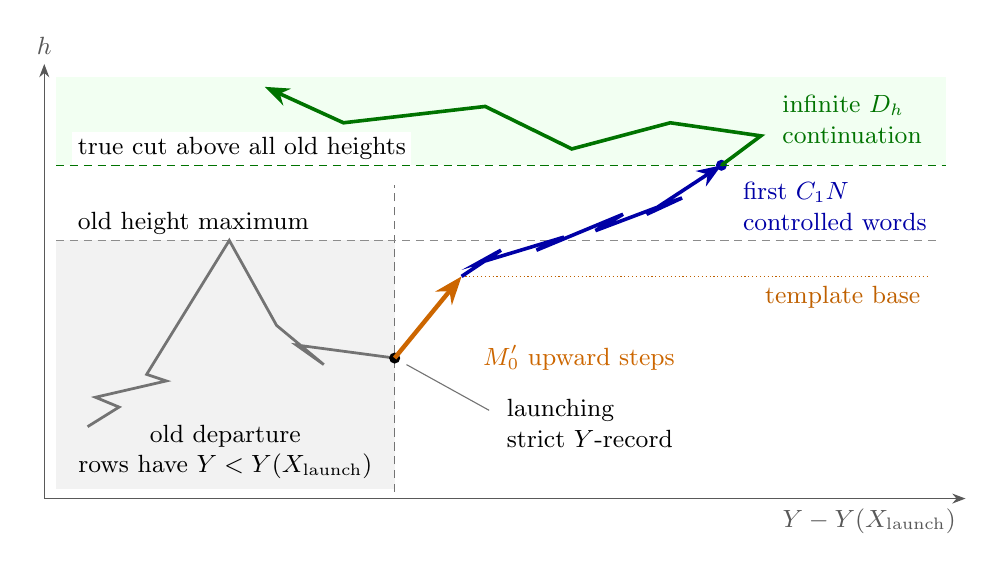
\begin{tikzpicture}[x=1cm,y=.83cm,font=\small,>=Stealth,
  old/.style={draw=black!55,line width=1pt},
  script/.style={draw=orange!80!black,line width=1.6pt},
  controlled/.style={draw=blue!65!black,line width=1.3pt},
  tail/.style={draw=green!45!black,line width=1.3pt}]
  \fill[black!5] (-4.3,.2) rectangle (0,4);
  \fill[green!5] (-4.3,5.15) rectangle (7,6.5);
  \draw[->,black!65] (-4.45,.05) -- (7.25,.05)
    node[below left] {$Y-Y(X_{\rm launch})$};
  \draw[->,black!65] (-4.45,.05) -- (-4.45,6.7) node[above] {$h$};
  \draw[densely dashed,black!55] (0,.15) -- (0,4.85);
  \draw[densely dashed,black!45] (-4.3,4) -- (6.9,4);
  \node[anchor=south west,fill=white,inner sep=2pt] at (-4.1,4)
    {old height maximum};
  \draw[old] (-3.9,1.15) -- (-3.5,1.45) -- (-3.8,1.6)
    -- (-2.9,1.85) -- (-3.15,1.95) -- (-2.1,4)
    -- (-1.5,2.7) -- (-.9,2.1) -- (-1.25,2.4) -- (0,2.2);
  \node[align=center,anchor=south] at (-2.15,.2)
    {old departure\\rows have $Y<Y(X_{\rm launch})$};
  \fill (0,2.2) circle (2pt);
  \draw[black!55] (.15,2.1) -- (1.2,1.4);
  \node[anchor=west,align=left] at (1.3,1.2)
    {launching\\strict $Y$-record};
  \draw[script,->] (0,2.2) -- (.85,3.45);
  \node[anchor=west,text=orange!80!black,align=left] at (1,2.2)
    {$M_0'$ upward steps};
  \draw[densely dotted,orange!75!black] (.85,3.45) -- (6.8,3.45);
  \node[anchor=north east,text=orange!75!black] at (6.8,3.45)
    {template base};
  \draw[controlled,->] (.85,3.45) -- (1.35,3.85) -- (1.05,3.65)
    -- (2.15,4.05) -- (1.8,3.85) -- (2.9,4.4)
    -- (2.55,4.15) -- (3.65,4.65) -- (3.2,4.4) -- (4.15,5.15);
  \node[anchor=west,align=left,text=blue!65!black] at (4.3,4.52)
    {first $C_1N$\\controlled words};
  \fill[blue!65!black] (4.15,5.15) circle (2pt);
  \draw[densely dashed,green!45!black] (-4.3,5.15) -- (7,5.15);
  \node[anchor=south west,fill=white,inner sep=2pt] at (-4.1,5.15)
    {true cut above all old heights};
  \draw[tail,->] (4.15,5.15) -- (4.65,5.6) -- (3.5,5.8)
    -- (2.25,5.4) -- (1.15,6.05) -- (-.65,5.8) -- (-1.65,6.35);
  \node[anchor=west,text=green!45!black,align=left] at (4.8,5.85)
    {infinite $D_h$\\continuation};
\end{tikzpicture}

\caption{The forward continuation in the $(Y,h)$ projection
(schematic, not to scale). Before launch, all departure rows have smaller
$Y$. The upward script raises the template base. The controlled words
stay beyond the old $Y$ maximum and above the script departures. Their
terminal true cut lies above all old heights; after that cut the suffix
may cross the old $Y$ barrier while still avoiding the old rows. The
projection does not restrict the walk to two dimensions.}
\label{fig:forward-template}
\end{figure}

It remains to bound the ratio on this continuation. The positive part
of the launch coordinate $u\cdot X_\sigma$, divided by any later
denominator, is at most $t+b+1$, since $h(X_\sigma)\ge0$ and the
denominator is nondecreasing. The later height term contributes at most
$b$. The script adds at most $M_0'$ to the ratio. In word $k+1$, the
additional coordinate contribution is at most
\[
\frac{M_0'/a+k+1}{A_0+ck}
\le\max\left\{\frac{M_0'+1}{A_0},\frac1c\right\},
\qquad A_0=1+M_0'-C_0>1.
\]
The numerator uses the bound on the sum of radii through word $k+1$;
the denominator uses the height of that word's starting boundary.
Thus any fixed
\[
K>2b+1+\max\left\{M_0',\frac{M_0'+1}{A_0},\frac1c\right\}
\]
proves the claim. Exit occurs by the last prescribed template endpoint.

\smallskip\noindent\emph{The exponential upper bound.}
Let $\sigma_j$ be the first crossing before $\zeta$ of
$t_j=1+jK$. The continuation just constructed prevents
$\sigma_{j+1}<\zeta$. Summing its bound over the finite prefixes at
$\sigma_j$ yields
\[
P_0(\sigma_{j+1}<\zeta)
\le(1-\epsilon_0)P_0(\sigma_j<\zeta).
\]
This conditions only on the observed crossing prefix; it does not reveal
whether an infinite template has failed. Hence the event in
\eqref{eq:3} has probability at most $C'e^{-c'B}$ for this $u$.
Taking the union over signed coordinates contradicts the lower bound
$p_hc_2/B$ when $B$ is large. All estimates use the permitted order:
fix the geometry constants, then $B$, then $i_0$, then take $a$ large.
This proves \eqref{eq:1}.
\end{proof}

\begin{corollary}[Deterministic limiting ray]\label{geom-ray}
There is a deterministic unit vector \(r\) with \(h(r)>0\) such that
\(X_n/\|X_n\|\to r\) almost surely. After a deterministic signed
permutation of the coordinate axes, \(r_1>0\), and all the preceding
word conclusions hold with height \(x_1\).
\end{corollary}

\begin{proof}
Word endpoints obey the vector strong law, with mean displacement
\(w\) satisfying \(h(w)=\mathbb E L>0\). Proposition~\ref{geom-radius}
also gives \(R_k/k\to0\) almost surely: for each \(\varepsilon>0\),
the probabilities \(\Pr(R_k>\varepsilon k)\) are summable. Thus
interpolation inside each word gives the same limiting direction
\(r=w/\|w\|\), without any duration moment. The completed-word count
tends to infinity. Lemma~\ref{geom-words} transfers the conclusion
through the finite initial raw prefix.

Some signed coordinate of \(r\) is positive. Relabel it as the first
coordinate, preserving the lattice, uniform ellipticity, and the iid
row law. Then \((X_n)_1\to+\infty\) almost surely. The proofs of
Lemma~\ref{geom-words} and Proposition~\ref{geom-radius} apply again
with this coordinate height, using only its transience. We retain the
same notation for the transformed walks and laws.
\end{proof}

\subsection{Layer notation; a small inverse moment}

Henceforth height means \(x_1\). Write \(x=(x_1,\underline x)\), \(\underline x\in\mathbb Z^{d-1}\); for fluctuations we use the single scalar coordinate \(x_2\). For a path from \(x\) and \(j\in\mathbb Z\), \(T_j=\inf\{n\ge0:(X_n)_1=x_1+j\}\) denotes first hit of the layer \(x_1+j\), relative to the indicated start (\(\inf\varnothing=\infty\); \(T_0=0\)). Put \(D=\{T_{-1}=\infty\}\), \(p=P_x(D)>0\),
\[
P_x^+=P_x(\,\cdot\,\mid D),\qquad q(x)=P_{x,\omega}(D),\qquad
a_H(x)=P_{x,\omega}(T_H<T_{-1})\quad(H\ge0\ \text{integer}),
\]
where the environment in notation such as \(q,a\) is implicit. Let \(K_H(x,\cdot)\) be the unnormalized quenched kernel of reaching that upper layer before the drop, of mass \(a_H(x)\); we also use it for the whole path prefix through this first hit, testing events on that prefix. It only uses rows in the \(H\) layers from the starting layer inclusive to the upper one exclusive. From 0 abbreviate \(a_H=a_H(0)\), \(u_H=E a_H\). The filtration \(\mathcal F_H\) on environments reveals rows at \(0\le x_1<H\); under \(P\) the upper layers from \(H\) inclusive are thus fresh iid layers, also starting at any finite \(\mathcal F_H\)-stopping layer (by partitioning according to that layer). Corresponding shifted filtrations at other bases will be used similarly. Write \(L_{\rm s},R_{\rm s},\tau_{\rm s}\) for the height width, radius and number of path steps in a single-walk true word in direction \(e_1\) under \(P_0^+\).

\begin{lemma}[A small inverse moment]\label{geom-inverse}
For every site \(x\), \(a_H(x)\downarrow q(x)>0\) for almost every
environment. Moreover, for some \(\lambda>0\),
\[
E\,q(0)^{-\lambda}<\infty. \tag{4}\label{eq:4}
\]
\end{lemma}

\begin{proof}
Uniform ellipticity excludes confinement forever in a fixed finite-height
strip, even quenched: blocks of sufficiently many consecutive upward
steps have a fixed positive chance. Hence \(a_H(x)\downarrow q(x)\).
Also \(q(je_1)\) uses only layers at or above \(j\), so the event that
\(q(je_1)>0\) infinitely often is a tail event of the independent layers.
For every \(m\), the union of these events over \(j\ge m\) has
probability at least \(P(q(0)>0)>0\), by stationarity and \(Eq(0)=p>0\).
The tail zero--one law makes their limsup almost sure. A finite upward
script connects zero to one such site and gives \(q(0)>0\). Translation
and countability give positivity at every site simultaneously.

At layer \(H\), let \(\mu_H=K_H(0,\cdot)/a_H\) be the endpoint
probability distribution. It is \(\mathcal F_H\)-measurable, and the
quenched Markov property, restricted to a suffix never below layer \(H\),
gives
\[
q(0)\ \ge\ a_H\int q(x)\,\mu_H(dx).
\]
Each \(q(x)\) on that layer has the original marginal law independently
of the lower rows. If \(q(0)/a_H<s\), then more than half the
\(\mu_H\)-mass has \(q(x)\le2s\). Conditional expectation followed by
Markov's inequality therefore gives
\[
P\big(q(0)/a_H<s\mid\mathcal F_H\big)
\le2P\big(q(0)\le2s\big).
\]
The endpoint values \(q(x)\) need not be independent of one another.
Partitioning by a finite stopping layer gives the same conditional bound
there.

Choose \(0<\delta<\kappa\) sufficiently small that
\(\rho:=2P(q(0)\le2\delta/\kappa)<1\), and set
\[
H_j=\inf\{H\ge0:a_H<\delta^j\},\qquad j\ge1.
\]
These are stopping layers. One upward step after a successful crossing
gives \(a_{H+1}\ge\kappa a_H\), so on \(H_j<\infty\),
\(a_{H_j}\ge\kappa\delta^j\). The event \(H_{j+1}<\infty\) implies
\(q(0)<\delta^{j+1}\), and hence
\(q(0)/a_{H_j}<\delta/\kappa\). The preceding conditional bound yields
\[
P(H_{j+1}<\infty\mid\mathcal F_{H_j})\le\rho
\quad\text{on }\{H_j<\infty\}.
\]
Since \(a_H\downarrow q(0)\), the event \(H_j<\infty\) is exactly
\(\{q(0)<\delta^j\}\). Iteration gives its probability at most
\(\rho^{j-1}\). Summing over
\(\delta^{j+1}\le q(0)<\delta^j\), and choosing \(\lambda>0\) with
\(\rho\delta^{-\lambda}<1\), proves \eqref{eq:4}.
\end{proof}

\subsection{Probability estimate sufficient for speed}

The rest of the paper will establish the following estimate for one
fixed \(0<\beta<1\):
\[
P(a_N<N^{-\beta})<N^{-D_0}
\quad\text{eventually for each fixed finite }D_0>0.
\tag{5}\label{eq:5}
\]

Small quenched exit probabilities also connect spatial estimates to
regeneration-time tails in Sznitman's
work~\cite[Lemma~3.2 and Theorem~3.3]{Sznitman2002}.
The next proposition gives the reduction for the crossing probabilities
defined here, with \eqref{eq:5} as its explicit input.

\begin{proposition}[From crossing probabilities to speed]\label{geom-speed}
If \eqref{eq:5} holds, then \(\mathbb E\tau_{\rm s}<\infty\), and
the walk has an almost-sure deterministic velocity with strictly positive
projection on the original direction \(\ell\).
\end{proposition}

\begin{proof}
All conclusions below using \eqref{eq:5} are conditional on that estimate.

\smallskip\noindent\emph{Spatial confinement before exit.}
The raw path before leaving the height interval \([0,N]\) stays in
\(\|\underline X\|_\infty\le CN^2\), except with probability at most
\(Ce^{-cN}\). To prove this, fix a signed lateral coordinate \(u\).
By Corollary~\ref{geom-ray}, a sufficiently large fixed \(b>0\) makes
\(Y(x)=u\cdot x+bx_1\) transient in its positive direction. Thus the
event of staying forever at \(Y\ge0\) has positive raw probability,
by the minimum argument of Lemma~\ref{geom-words}.

For a sufficiently large fixed \(C_2\), the path through its first
relative height hit \(N+1\) has norm at most \(C_2N\) with probability
tending to one. Indeed the ray gives
\(\|X_n\|\le(C_2/2)(X_n)_1\) eventually, and the earlier path has a
finite maximum norm. The intersection of this event with the preceding
no-backtracking event therefore has probability bounded below uniformly
for large \(N\).

At a first crossing of \(Y>jC_3N\), before strip exit, the walk is at
a strict \(Y\)-record. Impose that favorable translated suffix using
the fresh rows at or above the record. If \(C_3\) is sufficiently large,
the suffix precludes crossing \((j+1)C_3N\) before strip exit: its
\(Y\)-displacement through relative height \(N+1\) is at most
\((1+b)C_2N\), the launch overshoot is bounded, and absolute strip
exit occurs no later than this relative height hit. The finite-prefix
threshold recursion used in Proposition~\ref{geom-radius}, now with
spacing \(C_3N\), gives exponential decay through \(N\) thresholds.
Since \(u\cdot X\le Y\) before exit, the finite union over signed
lateral coordinates proves the confinement assertion.

\smallskip\noindent\emph{Super-polynomial width tails.}

Now \(\Delta u_N:=u_N-u_{N+1}\ge0\) is the annealed probability of reaching \(N\) before the drop but dropping before \(N+1\). In environments good at all sites of the strip and box (where \(a_{N+1}(x)\ge(N+1)^{-\beta}\)), the portion of this event inside the box has quenched probability at most
\[
(1-(N+1)^{-\beta})^{N+1}.
\]
Indeed, after reaching \(N\), at first descending-level visits to each of \(N,N-1,\ldots,0\) still in the box, there is at least the indicated chance to hit top \(N+1\) before the next descent by one. Condition \eqref{eq:5}, translation, a polynomial union bound, and the box claim thus give super-polynomial decay of \(\Delta u_N\).

The true levels under \(P_0^+\) form the renewal process of iid widths \(L_{\rm s}\), with renewal masses exactly \(u_n\): impose the fresh \(D\)-suffix at the first reach of \(n\) before drop, and cancel \(p\). If \(G_j=P_0^+(L_{\rm s}>j)\), then \(\sum_{j=0}^n G_j u_{n-j}=1\) by the last renewal up to \(n\), so
\[
G_{n+1}=\sum_{j=0}^n G_j\Delta u_{n-j}.
\]
Put \(f_k=\Delta u_{k-1}\) for \(k\ge1\). This nonnegative kernel has
total mass \(\theta=1-p<1\) and all polynomial moments. The recurrence,
with \(G_0=1\), gives \(G=\sum_{r\ge0}f^{*r}\), including unit mass
at zero for \(r=0\). If \(\theta>0\), normalize \(f\) by \(\theta\).
For every positive integer \(m\), the \(m\)-th moment of its
\(r\)-fold convolution is at most \(r^m\) times its \(m\)-th moment,
by
\((z_1+\cdots+z_r)^m\le r^{m-1}\sum_i z_i^m\).
Summing with the geometric weights \(\theta^r\) proves
\(\sum_n n^mG_n<\infty\). The case \(\theta=0\) is immediate.
In particular the width tail \(G_n\) decays super-polynomially.

\smallskip\noindent\emph{Time integrability and velocity.}
The raw exit time \(T_N\wedge T_{-1}\) exceeds \(N^A\) with
super-polynomially small probability, for a sufficiently large fixed
\(A\). To see this, use confinement and \eqref{eq:5} on a slightly
enlarged box and strip, requiring
\(a_N(x+e_1)\ge N^{-\beta}\) for every relevant site with
\(0\le x_1<N\). A polynomial union bound controls the exceptional
environments.

From any visit to such a site \(x\), the quenched probability of no
further visit before exit is at least \(\kappa a_N(x+e_1)\): take one
upward step and then advance \(N\) before dropping below the new layer.
This event forces original strip exit before revisiting \(x\), even
though the auxiliary target may be higher than \(N\). The quenched
Markov property consequently bounds each site's visit count by a
geometric tail with success probability at least \(\kappa N^{-\beta}\).
There are at most \(CN^{2d-1}\) sites in the confined box. If the exit
time exceeds \(N^A\), one site has at least
\(N^A/(CN^{2d-1})\) visits. For \(A>2d-1+\beta\), the union of these
geometric-tail events is super-polynomially small, as are the bad-box
and bad-environment events.

On \(D\), if \(L_{\rm s}\le N\), the first word ends at its first
arrival to height \(L_{\rm s}\), and hence
\(\tau_{\rm s}\le T_N\). Thus
\[
P_0^+(\tau_{\rm s}>N^A)
\le P_0^+(L_{\rm s}>N)
+p^{-1}P_0(T_N\wedge T_{-1}>N^A).
\]
Both terms have super-polynomial decay, proving
\(\mathbb E\tau_{\rm s}<\infty\). The iid-word strong laws now give
the velocity as mean displacement divided by mean duration; its first
coordinate is \(\mathbb E L_{\rm s}/\mathbb E\tau_{\rm s}>0\).
The integrable spatial radius controls the inter-endpoint deviations,
so this limit holds at every path time. The finite raw initial prefix
does not change it. Finally the velocity is a positive multiple of the
ray in Corollary~\ref{geom-ray}, which has positive projection on the
original \(\ell\). Undoing the signed coordinate permutation proves
the stated conclusion. As an almost-sure deterministic limit, this
velocity is unique for the law \(\nu\).
\end{proof}

It remains to prove \eqref{eq:5}. Sections~\ref{sec:fluctuations}--\ref{sec:stationary}
are devoted to that estimate; no finite duration moment is used there.

\section{Two-walk scales and preliminary comparisons}\label{sec:fluctuations}

We now measure fluctuations in the second coordinate at first hits of
successive height layers. Common true levels provide fresh pair
continuations and, for independent environments, an iid sequence of
symmetric increments. Their truncated variance will determine the
fluctuation scale. We first compare all first-hit positions with this
sequence, then transfer the comparison between two forms of conditioning.
The resulting short-block estimate and endpoint spread bounds will be
used in Sections~\ref{sec:gaussian} and~\ref{sec:clipping}.

On a successful prefix, set
\[
Y_j=(X_{T_j}-X_0)_2.
\]
Choose a deterministic integer median \(b_j\) of \(Y_j\) under \(P_0^+\),
with \(b_0=0\), and write
\[
W_H=\max_{0\le j\le H}|Y_j-b_j|.
\]
All these variables record displacement from the indicated starting site.

\subsection{Common true cuts}

Common spatial regeneration levels for two walks, reached at possibly
different path times, are central to the shared- and independent-environment
comparison of Rassoul-Agha and Sepp\"al\"ainen~\cite[Section~7]{RassoulAghaSeppalainen2009}.
Their invariance principle assumes regeneration-time moments. Here we
establish the common-cut identities directly from finite words, using the
spatial first moment proved in Section~\ref{sec:geometry}.

For two starting sites \(x,y\) on the same layer, we distinguish the
independent conditioned law \(P_x^+\otimes P_y^+\) from the annealed law
\(P_{x,y}^{++}\) of two walks in the same environment, conditioned on both
no-drop events \(D\). Let \(P_{x,y}^{\rm sh}\) denote the latter pair law
before conditioning, and put
\[
p_2(x,y)=E[q(x)q(y)].
\]
The positivity of \(q\) established in Section~\ref{sec:geometry} gives a
uniform lower bound
\[
\underline p_2:=\inf_{x_1=y_1}p_2(x,y)>0.
\]
Indeed, for every \(c>0\),
\[
P\bigl(\min(q(x),q(y))<c\bigr)\le 2P(q(0)<c),
\]
so a sufficiently small \(c\) makes \(q(x)q(y)\ge c^2\) on an event of
uniformly positive probability. Product-field mixing also gives
\[
p_2(x,y)\longrightarrow p^2
\qquad\text{as }\|x-y\|\longrightarrow\infty,\quad x_1=y_1.
\]
To verify this directly, approximate \(q(0)\) in \(L^1(P)\) by a bounded
function of finitely many rows and translate the approximation to \(x\)
and \(y\). The approximating functions are independent once their
translated row sets are disjoint.

Each marginal of the shared conditioned law is dominated uniformly by
the corresponding single conditioned law:
\[
P_{x,y}^{++}(X^{(1)}\in A)
 =\frac{E[P_{x,\omega}(A\cap D)q(y)]}{p_2(x,y)}
 \le \frac{p}{\underline p_2}P_x^+(A),
\]
and likewise for the second walk. With superscripts distinguishing the
walks, define
\[
\Delta_j=Y_j^{(2)}-Y_j^{(1)},\qquad
Z_j=y_2-x_2+\Delta_j.
\]
A \emph{common true level} is a level that is true for both walks at their
respective first hits. Heights are measured from the common starting
layer, and level zero is included under either conditioned law.

\begin{lemma}[Common words and their continuation laws]
\label{fluct-common-words}
Under either conditioned pair law, common true levels occur infinitely
often. At each such level the translated pair continuation is fresh:
under independent environments it has law \(P_0^+\otimes P_0^+\), while
under a shared environment, from terminal sites \(x',y'\), it has law
\(P_{x',y'}^{++}\) before translation. The latter transition law depends
on the terminal pair of sites.

These continuation rules remain valid at finite stopping indices of the
chain of common words, when the information retained consists of the
traversed words and their path prefixes.
\end{lemma}

\begin{proof}
Work first with the raw pair laws. Test a new integer level above both
explored path pasts, pausing each walk at its first arrival there. All
departure rows revealed by these prefixes lie strictly below the
candidate level. The conditional probability that both arrivals are
true is \(p^2\) in independent environments and \(p_2\) at the arrival
sites in a shared environment. Both probabilities have a uniform
positive lower bound.

If the candidate fails, resume the two walks, for example one step of
each per round, until one drops below the candidate. This failure is
detected in finite time. Then test a level strictly above both explored
pasts. Each walk tends to positive infinite height almost surely; this
also holds for the shared raw pair by its marginals. Thus, after every
detected failure, another candidate can be reached. The uniform success
bound proves the existence of a common true level above any prescribed
height. Conditioning on the two initial no-drop events preserves this
almost-sure conclusion.

For the continuation law, specify a pair of finite words from \(x,y\)
to their first hits \(x',y'\) of a common terminal level \(L>0\).
Call this word pair admissible when both prefixes avoid the initial
drop and every intermediate positive level has a witnessed failure of
common truth: at least one prefix has dropped below that level after its
first hit. These are exactly the required prefix conditions. Indeed,
once truth is imposed at \(L\), any failure of truth at an earlier level
must already have occurred in the specified prefixes.

Let \(A_{x,y}^{\rm sh}(w_1,w_2)\) be the raw annealed prefix weight of an
admissible word pair. Its quenched weight is the product of the two path
weights in the shared environment, including any repeated use of a row.
Every departure row lies below the terminal layer. The suffixes
constrained by truth use only rows at or above that layer, so site-row
independence gives the conditional word probability
\[
P_{x,y}^{++}\bigl((w_1,w_2)\text{ is the first common word}\bigr)
 =
 A_{x,y}^{\rm sh}(w_1,w_2)
 \frac{p_2(x',y')}{p_2(x,y)}.
\]
More generally, for any event \(B\) of the suffix pair, its joint
probability with this word pair is
\[
A_{x,y}^{\rm sh}(w_1,w_2)
\frac{p_2(x',y')}{p_2(x,y)}
P_{x',y'}^{++}(B).
\]
Here \(B\) is read with the new sites as starting sites. In particular,
the factor \(p_2(x',y')/p_2(x,y)\) is part of the shared word law; it
does not cancel in general.

In independent environments the corresponding terminal and initial
conditioning probabilities are both \(p^2\), so their ratio is one.
Translation of each walk separately then makes the relative suffix law
\(P_0^+\otimes P_0^+\), independent of the word just traversed. Enumerate
the countably many admissible finite word pairs and iterate these
factorizations to obtain the stated continuation rules. Summing over a
finite stopping index gives the same rules there. The information at
such an index does not include any unseen upper environment.
\end{proof}

In independent environments, let \(L\ge1\) be the integer width of a
common word and let \(S\) be its increment of \(\Delta\). The successive
pairs \((L_i,S_i)\), with their path decorations, are iid by
Lemma~\ref{fluct-common-words}. Exchanging the walks shows that \(S\) is
symmetric. In what follows, expectations of \(L,S\) refer to this
independent common-word law.

\begin{lemma}[Common-word moments and local tightness]
\label{fluct-local-tightness}
The independent common-word variables satisfy
\[
1\le \bar L:=\mathbb E L\le p^{-2},\qquad
\mathbb E|S|<\infty,\qquad \Pr(S\ne0)>0.
\]
For a single conditioned walk, and for either marginal of a shared
conditioned pair, the increments \(Y_{h+j}-Y_h\) are tight uniformly in
the deterministic level \(h\) when \(j\) ranges over any fixed bounded
set of nonnegative integers.

If \(\sigma(H)\) is the first common true level at or above \(H\) under
\(P_{x,y}^{++}\), then
\[
\sigma(H)-H,\quad
Y^{(i)}_{\sigma(H)}-Y^{(i)}_H\ (i=1,2)
\quad\text{are tight uniformly in }H,x,y.
\tag{6}\label{eq:6}
\]
At \(\sigma(H)\) the pair suffix has the shared conditioned law from its
new sites.
\end{lemma}

\begin{proof}
The probability that a deterministic level \(h\) is true under the
single conditioned law is \(u_h\), by the exact-truth identity in
Section~\ref{sec:geometry}. Independence therefore makes the renewal
mass for common words equal to \(u_h^2\ge p^2\). The renewal-count strong
law, including its infinite-mean version obtained by truncation, implies
\(\bar L\le p^{-2}\). The lower bound follows from \(L\ge1\).

For each of the two paths, let \(N_i\) be the number of its single words
used before the first positive common boundary. Since single widths are
positive integers, \(N_i\le L\). The event \(N_i\ge j\) is determined by
that path's first \(j-1\) words and the independent boundary sequence of
the other path. It is consequently independent of the radius of its
\(j\)-th word. The finite mean single-word radius from
Section~\ref{sec:geometry} gives
\[
\mathbb E\sum_{j=1}^{N_i}R_{{\rm s},j}^{(i)}
 =\mathbb E N_i\,\mathbb E R_{\rm s}
 \le \bar L\,\mathbb E R_{\rm s}<\infty.
\]
The absolute value of \(S\) is bounded by the sum of these two total
radii. Finally, uniform ellipticity permits two short paths with
different second-coordinate displacements to level one. Imposing fresh
truth there gives positive probability of an exact common cut with
nonzero \(S\).

We record the renewal estimate that supplies local tightness. For either
the single renewal sequence or the independent common sequence, let
\(L'\) be its word width and \(A\) any almost surely finite size of the
word, such as its maximal displacement. If \(A_{\rm word}\) is the size
of the word based at the last boundary at or below a deterministic
level \(h\), then
\[
\Pr(A_{\rm word}>s)
 \le \sum_{j=0}^h\Pr(L'>j,\ A>s)
 \le \mathbb E[L'\mathbf1_{\{A>s\}}].
\]
To obtain the first inequality, sum over the possible preceding
boundary levels \(h-j\), use independence of the next word, and bound
each renewal mass by one. Since \(\mathbb E L'<\infty\), the final
quantity tends to zero as \(s\to\infty\). The same reasoning with
\(A=L'\) gives tightness of the covering width. Thus first-hit positions
at a deterministic layer differ from their preceding boundary
positions by tight amounts. A fixed interval of integer levels meets
only the words covering those levels, so it also has tight total
displacement, uniformly in its base. Shared marginals inherit this
statement from their uniform domination by the single conditioned law.

It remains to prove \eqref{eq:6}. Test the \(m\) levels
\[
h=H,H+B,\ldots,H+(m-1)B.
\]
Call failure at \(h\) \emph{visible} if, after first hitting \(h\), some
walk drops below it before its first hit of \(h+B\). In the raw law,
the probability that all \(m\) tests have visible failure is at most
\((1-\underline p_2)^m\). Indeed, at each pair of first-hit arrivals to
\(h\), all previous visible-failure tests are already determined, while
both fresh truths at \(h\) would preclude the next failure. Passing to
the conditioned pair law costs at most \(\underline p_2^{-1}\).

If \(h\) is not common true but has no visible failure, some walk drops
below \(h\) after its first hit of \(h+B\). That walk has no single true
boundary between \(h\) and \(h+B\), inclusive; its word covering \(h\)
therefore has width greater than \(B\). The covering-word estimate and
marginal domination bound this alternative by
\[
C\mathbb E[L_{\rm s}\mathbf1_{\{L_{\rm s}>B\}}].
\]
A union bound over the \(m\) tests now gives
\[
P_{x,y}^{++}\bigl(\sigma(H)>H+(m-1)B\bigr)
 \le \underline p_2^{-1}(1-\underline p_2)^m
      +Cm\mathbb E[L_{\rm s}\mathbf1_{\{L_{\rm s}>B\}}].
\]
Choose \(m\) large and then \(B\) large. This proves uniform tightness of
the height overshoot. The fixed-interval displacement bound then proves
the other assertions in \eqref{eq:6}. Finally, the first common boundary
at or above \(H\) is a stopping index of the common-word chain, so its
suffix rule follows from Lemma~\ref{fluct-common-words}.
\end{proof}

\subsection{Truncated variance and median centering}

For \(r>0\), define
\[
m(r)=\mathbb E(S^2\wedge r^2),\qquad n(r)=r^2/m(r).
\]
These quantities are positive by \(\Pr(S\ne0)>0\). The scale \(n(r)\)
uses only the finite first moment of \(S\); a finite second moment is
not assumed.

\begin{lemma}[Scale and maximal estimates]\label{fluct-scales}
The function \(n\) is continuous and nondecreasing, tends to infinity,
and is strictly increasing for all sufficiently large \(r\). Write
\(r_s\) for its inverse on large scales, so \(n(r_s)=s\). Then
\[
n(cr)\ge c^2n(r)\ (0<c\le1),\qquad
n(r)\ge r/\mathbb E|S|.
\tag{7}\label{eq:7}
\]
For iid copies \(S_j\), let
\[
M_H^S=\max_{0\le i\le H}\left|\sum_{j=1}^iS_j\right|.
\]
Uniformly in integer \(H\ge0\) and \(z>0\),
\[
\mathbb E[(M_H^S)^2\wedge z^2]\le CHm(z),\qquad
\Pr(M_H^S>z)\le CH/n(z).
\tag{8}\label{eq:8}
\]
\end{lemma}

\begin{proof}
The ratio
\(m(r)/r^2=\mathbb E[(S^2/r^2)\wedge1]\) is continuous and
nonincreasing. There is a bounded interval of strictly positive values
of \(|S|\) having positive probability; its contribution is strictly
decreasing once \(r\) exceeds that interval. This proves the
monotonicity and eventual strict monotonicity of \(n\). Monotonicity of
\(m\) proves the first inequality in \eqref{eq:7}, and
\(S^2\wedge r^2\le r|S|\) proves the second, hence \(n(r)\to\infty\).

For \eqref{eq:8}, replace \(S_j\) by
\(S_j\mathbf1_{\{|S_j|\le z\}}\). These truncated variables have mean
zero by symmetry. The probability of any replacement among the first
\(H\) variables is at most \(H\Pr(|S|>z)\). Off this event the original
partial sums agree with the truncated sums, whose expected squared
maximum is at most
\(4H\mathbb E[S^2\mathbf1_{\{|S|\le z\}}]\) by the square maximal
inequality. On the replacement event, the capped squared maximum is
at most \(z^2\). Adding these bounds gives the first inequality in
\eqref{eq:8}; Markov's inequality for the capped square gives the
second.
\end{proof}

\begin{lemma}[Exact-level comparison]\label{fluct-exact-comparison}
For every integer \(H\ge0\) and \(z>0\),
\[
P_0^+(W_H>z)\le C\Pr(M_H^S>z).
\tag{9}\label{eq:9}
\]
No moment of the maximal decoration inside a common word is needed.
\end{lemma}

\begin{proof}
In a raw first walk, select the first level \(h\le H\), if any, such
that \(T_h<T_{-1}\) and \(|Y_h-b_h|>z\). Let \(A\) be the event that
such a level exists. Conditional on this prefix and its selected
level, an independent raw second walk reaches \(h\) before dropping,
with its displacement on the opposite side of the median \(b_h\),
with probability at least \(p/2\). Here the conditioned no-drop law
only lower bounds a prefix probability; it is not imposed as a
separate test on that second walk.

At the two first-hit endpoints, impose both fresh truths. Their
probability factor is \(p^2\). The resulting event implies the two
initial no-drop events and has \(h\) as an exact common true level,
with \(|\Delta_h|>z\). Dividing its raw probability by \(p^2\), its
probability under the independent conditioned pair law is at least
\(P_0(A)p/2\). At a common cut of height at most \(H\), the difference
is a partial sum of at most \(H\) common-word increments, so
\[
\Pr(M_H^S>z)\ge \frac p2P_0(A)
 \ge \frac{p^2}{2}P_0^+(W_H>z).
\]
This proves \eqref{eq:9}. All of these adaptive prefix transfers can
also be obtained by summing the corresponding finite stopped-word
identities separately over the possible levels \(h\).
\end{proof}

\begin{lemma}[Median linearization on short blocks]
\label{fluct-median-linearization}
For sufficiently small \(t>0\), uniformly in
\(1\le H\le tn(r)\),
\[
\max_{j\le H}|b_j-jb_H/H|\le C\sqrt t\,r.
\tag{10}\label{eq:10}
\]
\end{lemma}

\begin{proof}
By \eqref{eq:7}--\eqref{eq:9}, choose a fixed large \(C_0\), then
\(t\) small enough that \(C_0\sqrt t\le1\), to obtain
\[
P_0^+(W_{2H}>C_0\sqrt t\,r)<p/4.
\]
For \(i+j\le2H\), the event that \(i\) is exactly true under \(P_0^+\)
has probability \(u_i\ge p\), and its suffix has the fresh conditioned
law. There is therefore positive probability on this event that
\(Y_i\), \(Y_{i+j}\), and \(Y_{i+j}-Y_i\) are all within
\(C_0\sqrt t\,r\) of \(b_i\), \(b_{i+j}\), and \(b_j\), respectively.
For the first two requirements use the preceding maximal bound, and
for the third use the same bound on the fresh suffix. Consequently,
\[
b_{i+j}=b_i+b_j+O(\sqrt t\,r)
\qquad(i+j\le2H),
\]
uniformly in the indices.

Set \(d_j=b_j-jb_H/H\) for \(0\le j<H\). Apply the last relation to
\(j+j\), and, when \(2j\ge H\), also to \(H+(2j-H)\). This gives
\[
2d_j=d_{2j\bmod H}+O(\sqrt t\,r)
\]
with a uniform error. Taking the maximum absolute value over
\(0\le j<H\) bounds that maximum by half itself plus
\(C\sqrt t\,r\). Since the error at \(j=H\) is zero, this proves
\eqref{eq:10}.
\end{proof}

\subsection{Change of conditioning and short-block survival}

The estimates above concern \(P_x^+\), which conditions the joint
annealed law on no drop. Under that law environments are weighted by
\(q(x)/p\). For quenched kernel estimates we also need the mixture
\[
\widetilde P_x
 =\int P_{x,\omega}(\,\cdot\mid D)\,P(d\omega),
\]
which keeps the original environment law and conditions the path in
each environment separately. We first transfer large-scale fluctuation
bounds to this mixture. For blocks of height \(H\le tn(r)\), a fresh
restart after the first loss of mass will retain positive kernel mass
outside an environment exception of probability \(O(t^2)\).

\begin{lemma}[Transfer between conditioned laws]
\label{fluct-conditioning-transfer}
Along any sequences of integers \(H\ge0\) and real numbers
\(z\to\infty\),
\[
\limsup\widetilde P_0(W_H>z)
 \le C\limsup P_0^+(W_H>z/C)
\tag{11}\label{eq:11}
\]
with a fixed constant \(C\). If also \(H\to\infty\), the same bound
holds with the left-hand side evaluated under the \(P\)-average of
the normalized successful-prefix kernel \(K_H/a_H\) at the origin.
\end{lemma}

\begin{proof}
On the joint environment-and-path space,
\[
\frac{d\widetilde P_0}{dP_0^+}=\frac{p}{q(0)}.
\]
This density is integrable but need not be bounded. For any prescribed
error, truncate it and then approximate the truncation by a bounded
nonnegative environment function \(g\) depending on finitely many
rows. Thus \(g\) approximates \(p/q(0)\) in \(L^1(P_0^+)\), and
\(E_0^+g\) tends to one as the approximation error tends to zero.
We will remove the finite initial segment that can be affected by \(g\).

First check the deterministic centering error caused by such a removal.
If \(\limsup P_0^+(W_H>z/10)\ge0.3\), Equation~\eqref{eq:11}
is immediate with a sufficiently large fixed \(C\). Otherwise these
probabilities are eventually less than \(0.3\). For every fixed
integer \(s_0\), local tightness then gives
\[
|b_{h+s}-b_h|\le0.3z
\qquad(0\le s\le s_0,\ h+s\le H)
\]
for all sufficiently large indices in the sequence. Indeed, each of
\(|Y_h-b_h|\le z/10\) and
\(|Y_{h+s}-b_{h+s}|\le z/10\) has probability greater than \(0.7\).
By Lemma~\ref{fluct-local-tightness}, the probability of
\(|Y_{h+s}-Y_h|\le z/10\) tends to one uniformly over these indices.
The three events have a nonempty intersection, which proves the
claimed deterministic inequality by the triangle inequality.

Let \(s\) be the first positive single true boundary strictly above
every row used by \(g\). Its index in the single-word chain is a finite
stopping index. For a sufficiently accurate approximation, \(E_0^+g>0\).
Under the probability measure with density \(g/(E_0^+g)\) relative to
\(P_0^+\), the translated suffix at \(s\) has law \(P_0^+\),
independently of the prefix. To verify this, apply exact-word
factorization separately to each finite prefix through the selected
boundary. Both its path weight and \(g\) use only rows below that
boundary; all rows for the conditioned suffix are fresh. This remains
true for rows used by \(g\) that the prefix has not visited. The
separation is by height, not by which rows the walk happened to reveal.

For fixed \(g\), first choose a deterministic \(s_0\) so large that
\(s\le s_0\) except for an arbitrarily small \(g\)-weighted error.
As \(z\to\infty\), we may further restrict to
\[
\max_{j\le s}|Y_j|\le z/10,
\qquad \max_{j\le s_0}|b_j|\le z/10,
\]
with a further error tending to zero. On these restrictions no offense
\(|Y_j-b_j|>z\) can occur before \(s\). After \(s\), write the
relative suffix displacement as \(Y'_u=Y_{s+u}-Y_s\). The centering
estimate above gives, for \(s<j\le H\),
\[
|Y_j-b_j|
\le |Y_s|+|Y'_{j-s}-b_{j-s}|+|b_{j-s}-b_j|
\le0.4z+|Y'_{j-s}-b_{j-s}|.
\]
Thus \(W_H>z\) requires the fresh suffix to have its own
\(W_H>z/10\). If \(H\le s\), no offense remains at all.

The \(g\)-weighted probability is consequently bounded in the limsup
by \(E_0^+g\) times \(\limsup P_0^+(W_H>z/10)\), plus the
restriction errors. Return to \(\widetilde P_0\) using the
\(L^1\) density approximation, and send all approximation and
restriction errors to zero. Enlarging the same fixed \(C\) to include
the earlier trivial case proves Equation~\eqref{eq:11}.

Finally, in a fixed environment the event \(D\) is a subevent of
\(\{T_H<T_{-1}\}\). On first-hit prefixes, changing between these
two conditional laws costs total variation at most \(1-q(0)/a_H\).
Therefore the distance between \(\widetilde P_0\) on those prefixes
and the \(P\)-average of \(K_H/a_H\) is at most
\[
E(1-q(0)/a_H)\longrightarrow0,
\]
since \(a_H\downarrow q(0)>0\) almost surely. This proves the last
assertion.
\end{proof}

\begin{proposition}[Short-block survival]
\label{fluct-short-block}
For every \(v_0>0\) there are constants \(C_{v_0}<\infty\) and
\(t_{v_0}>0\) such that, for each fixed \(0<t\le t_{v_0}\), some
\(\delta>0\) satisfies, for all sufficiently large \(r\), every
integer \(1\le H\le tn(r)\), and every probability measure \(\pi\)
on a starting layer,
\[
P\left(
 \pi K_H\{W_H\le v_0r,\
       \max_{j\le H}|Y_j-jb_H/H|\le v_0r\}<\delta
 \right)
 \le C_{v_0}t^2.
\tag{12}\label{eq:12}
\]
The environment is fresh with product law, and path displacements
are measured from each path's own starting site.
\end{proposition}

\begin{proof}
Fix \(v_0>0\), set \(w_0=v_0/8\), and write
\(\theta=b_H/H\). The proof uses one estimate for loss of mass in a
narrower slope tube, then restarts that estimate after its first failure.
All stopping tests will use finite-height kernels.

\paragraph{One possible loss of mass.}
Choose \(t_{v_0}\) small enough that Equation~\eqref{eq:10} gives,
for sufficiently large \(r\), uniformly over the stated \(H\),
\[
\max_{j\le H}|b_j-j\theta|\le w_0r/2,
\qquad |\theta|\le w_0r.
\]
The second inequality follows from the first at \(j=1\), since
\(b_1\) is fixed. Equations~\eqref{eq:7}--\eqref{eq:9} and
\eqref{eq:11} also give
\[
E[P_{0,\omega}(W_H>w_0r/2\mid D)]\le C_{v_0}t
\]
uniformly in \(1\le H\le tn(r)\) for large \(r\). Indeed, a
violating sequence of \(H,r\) would contradict the limsup transfer
in Equation~\eqref{eq:11}, whose right side is bounded by a constant
times \(H/n(r)\). The scale inequality in Equation~\eqref{eq:7}
absorbs the fixed change in threshold.

Choose \(\delta_0\in(0,1/4)\) so that
\(P(q(0)<4\delta_0)\le t\). Call a starting site \(x\) favorable
when
\[
q(x)\ge4\delta_0,
\qquad P_{x,\omega}(W_H\le w_0r/2\mid D)\ge1/2.
\]
The expected \(\pi\)-fraction of unfavorable sites is at most
\(C_{v_0}t\). Markov's inequality shows that, except on an environment
event of probability at most \(C_{v_0}t\), favorable sites carry at
least half the initial mass. From each favorable site the raw mass of
paths on \(D\) in the median tube is at least \(2\delta_0\).
Their first-hit prefixes lie in the slope tube of width \(w_0r\) at
every shorter horizon. Hence, except on that one environment event,
\[
M_u^\pi:=
\pi K_u\left\{\max_{j\le u}|Y_j-j\theta|\le w_0r\right\}
\ge\delta_0
\qquad(0\le u\le H).
\]
In particular the probability that any of these inequalities fails is
at most \(C_{v_0}t\), uniformly in the initial probability \(\pi\).
No independence among the environments seen from different starting
sites was used.

\paragraph{A fresh restart after the first failure.}
Test the masses \(M_u^\pi\) in increasing order, and let \(s\) be
the first level at which the displayed inequality fails. There is no
failure at level zero, since \(M_0^\pi=1\). Each test is measurable
from rows strictly below its tested layer, so \(s\le H\), when finite,
is an environment stopping layer.

The passing submeasure at layer \(s-1\) has mass at least
\(\delta_0\). Extend every one of its prefixes by one direct
\(+e_1\) step. Uniform ellipticity leaves mass at least
\(\kappa\delta_0\). The extension has slope error at most
\(2w_0r\), since the earlier error is at most \(w_0r\) and
\(|\theta|\le w_0r\). Both detection of the failure and this bridge
use only rows below layer \(s\).

Normalize the bridged endpoint submeasure to a probability \(\pi_s\)
and restart at layer \(s\). Conditional on the exposed lower rows,
\(\pi_s\) is fixed and the upper field has its original product law.
The one-failure estimate therefore applies again. Use the same slope
\(\theta=b_H/H\) and its original horizon \(H\); its simultaneous
conclusions imply the required ones through the shorter remaining
horizon \(H-s\). Replacing \(H\) by \(H-s\) in the slope would
not be justified and is unnecessary.

Thus, conditional on the first failure, the probability of a second
failure before the remaining horizon is at most \(C_{v_0}t\).
The probability of two failures is at most \(C_{v_0}t^2\), after
enlarging the constant. This multiplication uses fresh upper rows at
the stopping layer, not independence of two events in the original slab.

\paragraph{Retained mass and its tube.}
If no first failure occurs, at least \(\delta_0\) of the original
kernel mass reaches the top in the slope tube. If there is a first
failure but no second one, concatenate the bridged mass and the restarted
successful prefixes. Retain each prefix's original starting site when
doing so; restarted displacements are measured from the new endpoint.
The total slope error is at most \(2w_0r+w_0r=3w_0r\), and the
retained mass is at least \(\kappa\delta_0^2\). Local no-drop
successes are also successes above the original floor, so the
concatenated kernels are submeasures of the original \(K_H\).

Adding the deterministic median-line error \(w_0r/2\) puts these
prefixes in the required median tube as well. Both tube widths are
less than \(v_0r\). Take
\(\delta=\min\{\delta_0,\kappa\delta_0^2\}\) to obtain
Equation~\eqref{eq:12}. The infinite no-drop event served only to bound
failure probabilities; every test, bridge, and restart used the
finite-height prefix kernels.
\end{proof}

\subsection{Endpoint spread}

\begin{lemma}[Spread at the truncated-variance scale]
\label{fluct-endpoint-spread}
Under the independent conditioned pair law, there is a constant
\(c>0\) such that
\[
\begin{split}
&\Pr(|\Delta_{\lfloor n(r)\rfloor}|>cr)\ge c
       \qquad(r\ \text{large}),\\
&\liminf\Pr(|\Delta_{\lfloor tn(r)\rfloor}|>lr/4)
       \ge c_{l,\epsilon}t
 \quad\text{if }r\to\infty,\qquad
       n(r)\Pr(|S|>lr)\ge\epsilon.
\end{split}
\tag{13}\label{eq:13}
\]
In the second assertion \(0<l<1\) and \(\epsilon>0\) are fixed,
and the bound holds for each sufficiently small fixed \(t>0\),
depending on \(l,\epsilon\). Relative to any deterministic endpoint
center, a single \(P^+\)-walk consequently has a comparable
probability of a deviation, at half the corresponding separation
threshold, in at least one of the two signs.
\end{lemma}

\begin{proof}
Fix \(s>0\), put \(H=\lfloor sn(r)\rfloor\), and let
\(k=\lfloor H/\bar L\rfloor\). First we justify the approximation
\[
\Delta_H-\sum_{i=1}^kS_i=o_{\Pr}(r).
\]
By Lemma~\ref{fluct-local-tightness}, the displacement from the
preceding common boundary to the first-hit position at \(H\) is
tight. The renewal strong law puts the number of completed common
words within \(o_{\Pr}(n(r))\) of \(k\). No independence between
this count and the increments is required: on the event that its
distance from \(k\) is at most \(an(r)\), bound the sum error by
the maximal sums in the deterministic forward and backward
windows of that length around \(k\). For every fixed
\(\rho>0\), \eqref{eq:7}--\eqref{eq:8} bound the probability of
such an error exceeding \(\rho r\) by
\(O_\rho(a)+o(1)\). Let \(a\downarrow0\), and include the tight
decoration error, to obtain the approximation.

For \(s=1\), set
\[
V=\sum_{i=1}^k(S_i^2\wedge r^2).
\]
Its mean is comparable to \(r^2\), since
\(k\sim n(r)/\bar L\), and
\[
\mathbb E V^2
 \le kr^2m(r)+k^2m(r)^2=O(r^4).
\]
The second-moment inequality therefore makes \(V\) exceed a fixed
positive multiple of \(r^2\) with uniformly positive probability.
Conditional on the magnitudes \((|S_i|)\), the nonzero signs are
independent fair signs. The sum \(\sum_{i=1}^kS_i\) has conditional
variance \(Q=\sum_{i=1}^kS_i^2\ge V\) and conditional fourth
moment at most \(3Q^2\). A further second-moment inequality gives
a uniformly positive conditional probability of a displacement
of order \(\sqrt Q\), hence of order \(r\) on the preceding event.
The approximation, with a smaller displacement constant, proves
the first line of \eqref{eq:13}.

For the second line, take \(s=t\) and set
\(p_r=\Pr(|S|>lr)\). The assumptions and the definition of \(m\)
give
\[
\epsilon\le n(r)p_r\le l^{-2}.
\]
Among \(k\sim tn(r)/\bar L\) summands, the probability that exactly
one has magnitude greater than \(lr\) is therefore at least
\(c_{l,\epsilon}t\) for each sufficiently small fixed \(t>0\) and
large \(r\). Conditional on the index of that exceptional
summand, the others are independent symmetric variables
conditioned to have magnitude at most \(lr\). Their sum has
variance at most
\[
\frac{k\,\mathbb E[S^2\mathbf1_{\{|S|\le lr\}}]}{1-p_r}
 \le Ctr^2.
\]
For \(t\) sufficiently small, Chebyshev's inequality gives
probability at least \(1/2\) that their sum has magnitude at most
\(lr/2\). On this event they cannot cancel more than half the
exceptional summand. Thus the deterministic sum has magnitude
greater than \(lr/2\) with probability at least a constant times
\(t\). Keep \(t\) fixed while \(r\to\infty\); the
\(o_{\Pr}(r)\) approximation then proves the claimed bound at
threshold \(lr/4\).

Finally, if two iid endpoint displacements differ by more than
\(a\), at least one differs from any given deterministic center
by more than \(a/2\). The probability of this single-walk
absolute deviation is at least half the two-walk separation
probability. One of its two signs has at least half that mass.
This proves the final assertion after adjusting constants.
\end{proof}

\section{Gaussian scales}\label{sec:gaussian}

We next identify the fluctuation law on scales where the independent
common-word increments have negligible large jumps. There are three
steps: an annealed limit for independent paths, a comparison for shared
paths away from one another, and an occupation estimate excluding a
singular interaction on their projected diagonal. The resulting shared
two-copy limit will imply a quenched limit in probability.

\begin{definition}[Gaussian sequence]\label{gauss-sequence}
A sequence \(r\to\infty\) is \emph{Gaussian} if
\[
n(r)\Pr(|S|>a r)\longrightarrow0\qquad\text{for every fixed }a>0.
\tag{14}\label{eq:14}
\]
\end{definition}

Throughout this section limits are along any fixed Gaussian sequence.
Height-indexed processes are linearly interpolated on the grid
\(h/n(r)\). Functional convergence means weak convergence in
\(C([0,T],\mathbb R^k)\), with the uniform norm, for every fixed finite
\(T\); a slightly larger horizon is used when interpolating near its
endpoint. Put \(\sigma_*^2=1/(2\bar L)\).

\subsection{Independent-path Brownian limit}

The common-word increments give a Brownian limit at common cuts. To
obtain a limit for a single walk at every first-hit level, we must also
control the fluctuations between cuts and recover the deterministic
centering. Neither step requires a second moment for word decorations.

\begin{lemma}[Independent first-hit fluctuations]\label{gauss-independent}
For two independent conditioned paths, \(\Delta_h/r\) converges
functionally to Brownian motion of variance parameter \(1/\bar L\).
For a single \(P_0^+\) path, \((Y_h-b_h)/r\) converges functionally to
Brownian motion of variance parameter \(\sigma_*^2\).
\end{lemma}

\begin{proof}
Write \((L_i,S_i)\) for the successive independent common-word widths
and difference increments, and put
\[
 C_m=\sum_{i=1}^mL_i,\qquad A_m=\sum_{i=1}^mS_i,
 \qquad N(h)=\max\{m:C_m\le h\}.
\]
The difference at the preceding common cut is
\(\widehat\Delta_h=A_{N(h)}\). As with the first-hit process, we
interpolate its values linearly on the height grid \(h/n(r)\).

\emph{The limit at common cuts.}
First consider \(A_m/r\), with \(n(r)\) summands per unit time.
The Gaussian-sequence assumption permits a symmetric truncation
\[
 S_i^{(r)}=S_i\mathbf1_{\{|S_i|\le\eta_r r\}},
 \qquad \eta_r\downarrow0,
\]
for which
\[
 n(r)\Pr(|S|>\eta_r r)\longrightarrow0,
 \qquad
 \frac{\mathbb E[(S_i^{(r)})^2]}{m(r)}\longrightarrow1.
\]
Indeed, for every fixed \(0<\eta<1\),
\[
 0\le m(r)-\mathbb E[S^2\mathbf1_{\{|S|\le\eta r\}}]
 \le r^2\Pr(|S|>\eta r)=o(m(r));
\]
a sufficiently slow diagonal choice of \(\eta_r\) gives both
requirements. The probability that any summand is removed on a fixed
time interval tends to zero.

The variables \(S_i^{(r)}/r\) have mean zero, variance
\((1+o(1))/n(r)\), and fourth moment at most \(\eta_r^2\) times
that variance. Taylor expansion of their characteristic functions
therefore gives the standard Brownian finite-dimensional laws. For
tightness, the fourth-moment computation for independent centered sums,
followed by the fourth-moment maximal inequality, bounds the expected
maximal fourth power on a block of \(\lfloor\delta n(r)\rfloor\)
summands by
\[
 O(\delta^2+\delta\eta_r^2).
\]
A union bound over the blocks in a fixed time interval, followed by
\(\delta\downarrow0\), proves tightness. Thus \(A_m/r\) has the
standard Brownian functional limit.

The width strong law gives
\[
 \sup_{0\le h\le Tn(r)}
 \left|\frac{N(h)}{n(r)}-\frac{h}{\bar L n(r)}\right|
 \longrightarrow0
 \quad\text{in probability}.
\]
Applying this time change to the tight sum process, whose limits are
continuous, proves the Brownian limit for
\(\widehat\Delta_h/r\), with variance parameter \(1/\bar L\).
The counts and the sums need not be independent. The maximal normalized
jump tends to zero as well, so the stated interpolation convention has
the same limit.

\emph{Passing from cuts to every first hit.}
Lemma~\ref{fluct-local-tightness} makes
\(\Delta_h-\widehat\Delta_h\) tight uniformly at deterministic
levels \(h\). This already gives the required finite-dimensional
limits. To prove path tightness, fix \(\delta>0\) and partition the
height range into consecutive blocks of
\(\lfloor\delta n(r)\rfloor\) levels. There are only finitely many
block starts for fixed \(T,\delta\).

Suppose that within one of these blocks, with start \(a\),
\[
 |\Delta_h-\Delta_a|>\rho r
\]
for some level \(h\) in the block. Under the raw independent pair
law, select the first such offending level among prefixes for which
both walks have avoided the initial drop. The selection is determined
by the paired prefixes through that level. The raw probability of
finding an offense is at least \(p^2\) times its probability under
the independent conditioned pair law. Imposing both fresh truths at
the selected level multiplies each selected prefix weight by \(p^2\),
leaves the offense unchanged, and implies both initial no-drop events.
After division by the initial normalizer \(p^2\), both probabilities
below are under the conditioned pair law, and
\[
 \Pr(\text{an offense})
 \le p^{-2}\Pr(\text{an offense at a common cut}).
\]
The same statement holds for the union of the blocks by selecting its
first offense.

At a common cut \(h\), the offending difference satisfies
\[
 |\Delta_h-\Delta_a|
 \le |\widehat\Delta_h-\widehat\Delta_a|
       +|\Delta_a-\widehat\Delta_a|.
\]
The maximum of the second term over the finitely many deterministic
block starts is \(o_{\Pr}(r)\). The first term is controlled by the
modulus of the common-cut process, which has a continuous Brownian
limit. Consequently, for each \(\rho>0\), the limsup probability of
an offense tends to zero as \(\delta\downarrow0\). Adjacent-block
bounds and interpolation give tightness of \(\Delta_h/r\), proving
the first assertion.

\emph{Recovering a single path.}
Let \(\mu_r\) be the law in continuous path space of the interpolated
single-path process \(Y_h/r\), on a fixed compact time interval. Its
iid differences are tight by the first assertion. We first show that
\(\mu_r\) is tight after suitable deterministic path translations.
Choose compact sets \(K_j\) capturing the difference laws with errors
\(\varepsilon_j^2\), where \(\varepsilon_j\downarrow0\) and
\(\sum_j\varepsilon_j<1\). If a prospective center \(f\) is sampled
from \(\mu_r\), then
\[
 \int\mu_r(f+K_j)\,\mu_r(df)\ge1-\varepsilon_j^2.
\]
Markov's inequality shows that the centers for which
\(\mu_r(f+K_j)<1-\varepsilon_j\) have \(\mu_r\)-probability at
most \(\varepsilon_j\). Some center path \(f_r\) therefore works
for every \(j\), and the translated laws are tight. We may choose
\(f_r\) with the same interpolation as the original paths.

Along a subsequence on which these translated laws converge, let
\(G\) be the continuous limiting process. Its iid two-copy difference
has the Brownian law just proved. Cram\'er's normal decomposition
principle~\cite{Cramer1936}, in the iid-difference form verified below,
applied to every scalar linear combination of finitely many coordinates
of \(G\), shows that \(G\) has Gaussian finite-dimensional laws.
Its covariance is half that of the difference process, namely
\[
 \operatorname{Cov}(G(s),G(t))=\sigma_*^2\min(s,t).
\]
Only a deterministic mean function remains to be identified.

For completeness, suppose that \(Z-Z'\) is normal for iid real
variables \(Z,Z'\). Choose \(C_0\) with
\(\Pr(|Z'|\le C_0)>0\). Intersecting either tail of \(Z\) with
this event bounds that tail by a constant times a Gaussian tail. Hence
\(f(z)=\mathbb E e^{zZ}\) is entire and obeys
\(|f(z)|\le\exp(C(1+|z|^2))\). The identity
\(f(z)f(-z)=\mathbb E e^{z(Z-Z')}\), first on the real axis and
then everywhere, shows that \(f\) has no zeros. Its entire logarithm
\(g\), chosen with \(g(0)=0\), satisfies
\(\operatorname{Re}g(z)\le C(1+|z|^2)\). On every circle the mean
of \(\operatorname{Re}g\) is zero, so its absolute integral mean is
also \(O(1+|z|^2)\). The Fourier coefficient formula on circles of
arbitrarily large radius then makes every Taylor coefficient of \(g\)
of order greater than two vanish. Thus \(g\) is quadratic, real on
the real axis, with \(g''(0)=\operatorname{Var}Z\ge0\). It follows
that \(Z\) is normal, allowing a point mass.

Write \(m_G(t)=\mathbb E G(t)\). Sample continuity and convergence
in law of Gaussian marginals at convergent times imply that \(m_G\)
is continuous. Each marginal has the unique median \(m_G(t)\),
including at time zero. At a grid time \(h/n(r)\), the number
\[
 \frac{b_h}{r}-f_r(h/n(r))
\]
is a median of the translated marginal. Along every sequence of grid
times converging to \(t\), weak path convergence and uniqueness of
the limiting median make these medians converge to \(m_G(t)\).
Compactness of the time interval makes the convergence uniform over
grid times; interpolation gives uniform convergence on the whole
interval. Use a slightly longer interval when interpolating at the
endpoint. Subtracting the interpolated medians from the original
process therefore removes precisely the limiting mean function.
Every subsequential limit is Brownian motion of variance parameter
\(\sigma_*^2\), proving the single-path assertion.
\end{proof}

\begin{lemma}[Linearization of the medians]\label{gauss-medians}
Uniformly for \(k+j\le T n(r)\), for each fixed \(T\),
\[
 b_{k+j}-b_k-b_j=o(r).
 \tag{15}\label{eq:15}
\]
Writing \(N_r=\lfloor n(r)\rfloor\) and
\(\theta_r=b_{N_r}/N_r\), we have
\[
 \max_{h\le Tn(r)}|b_h-h\theta_r|=o(r),
 \qquad \theta_r=o(r).
\]
\end{lemma}

\begin{proof}
We first prove the additive relation. It suffices to consider arbitrary
sequences of indices for which
\(k/n(r)\to s\) and \(j/n(r)\to t\), and to pass further so
that \(k\) is fixed or tends to infinity. Let \(\mathcal C_k\)
be exact single truth at level \(k\). Under \(P_0^+\), this event
has probability \(u_k\ge p\). Conditional on \(\mathcal C_k\),
the prefix has the raw law conditioned on \(T_k<T_{-1}\), and its
relative suffix is an independent fresh \(P_0^+\) path.

If \(k\to\infty\), the total variation distance between this
prefix law and the \(P_0^+\) prefix law is at most
\(1-p/u_k\to0\). If \(k\) is fixed, its displacement and median
are fixed random and deterministic quantities, respectively, and their
normalized difference tends to zero. Lemma~\ref{gauss-independent}
therefore gives, under the conditional law,
\[
 \frac{Y_{k+j}-b_k-b_j}{r}
 \ \Longrightarrow\ N(0,\sigma_*^2(s+t)).
\]
The same lemma gives this normal limit under the unconditional
\(P_0^+\) law when the centering is \(b_{k+j}\).

Set \(d_r=(b_k+b_j-b_{k+j})/r\). The unconditional distribution
centered by \(b_{k+j}\) dominates \(p\) times the conditional
distribution with that same centering. Tightness first forces \(d_r\)
to be bounded. Along a further subsequence with \(d_r\to d\), the
limiting domination would read
\[
 N(0,v)\ \ge\ pN(d,v),\qquad v=\sigma_*^2(s+t),
\]
as measures. For \(v>0\), a nonzero shift makes the ratio of the
shifted normal density to the unshifted one unbounded. For \(v=0\),
the two point masses have different supports unless \(d=0\).
Thus \(d=0\) in every case. Compactness of the ranges of
\(k/n(r)\) and \(j/n(r)\) proves the uniform relation
\eqref{eq:15}.

To turn approximate additivity into a linear approximation, put
\(N=N_r\), \(\theta=b_N/N\), and
\(d_j=b_j-j\theta\) for \(0\le j<N\). Apply \eqref{eq:15}
to \(j+j\), and also to \(N+(2j-N)\) when \(2j\ge N\).
Uniformly over these indices,
\[
 2d_j=d_{2j\bmod N}+o(r).
\]
The maximum of \(|d_j|\) is therefore at most half itself plus
\(o(r)\), so it is \(o(r)\). For \(h\le Tn(r)\), write
\(h=qN+j\), where \(q\) remains bounded, and apply
\eqref{eq:15} a bounded number of times. This proves
\(\max_{h\le Tn(r)}|b_h-h\theta_r|=o(r)\). Finally, at \(h=1\)
this gives \(|b_1-\theta_r|=o(r)\); since \(b_1\) is fixed,
\(\theta_r=o(r)\).
\end{proof}

\subsection{Shared paths: marginals and separation}

Two paths in one environment interact when their traces visit a common
site. We first show that the conditioning on the second path does not
change the limiting fluctuations of the first. We then bound trace
contact by the probabilities of missing two disjoint endpoint windows.
This comparison concerns the entire traces, including their excursions
between first hits of successive layers.

\begin{lemma}[Shared marginal limits]\label{gauss-shared-marginals}
Under \(P_{x,y}^{++}\), each marginal process
\[
B_i^r(h/n(r))=(Y_h^{(i)}-h\theta_r)/r
\tag{16}\label{eq:16}
\]
converges functionally to Brownian motion of variance parameter
\(\sigma_*^2\), uniformly over starts on a common layer. Thus the
conclusion holds along every choice \(x=x(r),y=y(r)\) with
\(x_1=y_1\), whatever their separation. The pair is jointly tight.
\end{lemma}

\begin{proof}
Relative to the single conditioned environment-and-path law from \(x\),
the first marginal has density
\[
\frac{p\,q(y)}{p_2(x,y)}.
\]
For a fixed integer \(J\), replace \(q(y)\) by \(a_J(y)\), then
normalize. The resulting probability law differs from the original
one in total variation by at most \(C(u_J-p)\), uniformly in \(x,y\).
Indeed \(a_J\ge q\), and the added mass before normalization is
\[
\frac{E[q(x)(a_J(y)-q(y))]}{p_2(x,y)}
\le\frac{u_J-p}{\underline p_2}.
\]
All these normalized laws have density bounded by a common constant
relative to the single conditioned law.

The weight \(a_J(y)\) uses only rows between the common base and the
layer \(J\) above it, excluding the latter. Stop the single-word chain
of the first walk at its first true boundary at or above that layer.
Every row used by the weight lies below this boundary. Exact-word
factorization therefore gives a fresh \(P^+\) suffix, independent of
the removed path prefix under the weighted law. The weight may depend
on infinitely many sites in those \(J\) layers; only their heights
matter for this factorization.

For fixed \(J\), the height and size of this initial prefix are tight
under \(P_x^+\), and hence under every one of the bounded weighted laws.
Its height divided by \(n(r)\) tends to zero. Its displacement divided
by \(r\) also tends to zero, as does its centering correction, since
\(\theta_r/r\to0\). The suffix limit and its tight continuous modulus
thus give the asserted limit under the approximating law. Send
\(r\to\infty\) first and then \(J\to\infty\). The same proof applies
to the second marginal, and tightness of the two marginals gives joint
tightness.
\end{proof}

The next elementary observation converts endpoint concentration into a
bound on trace contact. Fix an environment and a base layer of height
\(F\). Let each walk be conditioned never to fall below \(F\), and
stop it on first arrival at height \(F+k\). For disjoint sets
\(I_1,I_2\) in that top layer, write \(E_i\) for the event that walk
\(i\)'s endpoint lies outside \(I_i\). Then
\[
P_{x,\omega}(\,\cdot\mid D)\otimes
P_{y,\omega}(\,\cdot\mid D)
 \{\text{the two stopped traces meet}\}
\le 2P_{x,\omega}(E_1\mid D)+2P_{y,\omega}(E_2\mid D).
\]
Here the two occurrences of \(D\) use the same absolute floor \(F\).
To prove the bound, for \(F\le z_1\le F+k\) let \(v_i(z)\) be the probability of a top endpoint
in \(I_i\) for a quenched walk from \(z\) conditioned to avoid that
floor. We consider only sites with positive probability of such
avoidance. The Markov property makes \(v_i(z)\) the conditional endpoint
probability whenever either walk first visits \(z\), regardless of
which walk visits it. Since \(I_1,I_2\) are disjoint,
\(v_1(z)+v_2(z)\le1\).

Put \(A_i=\{z:v_i(z)\le1/2\}\). At the first visit to \(A_i\) before
or at the top, the conditional probability of \(E_i\) is at least
\(1/2\). The quenched Markov property at that first visit gives
\[
P_{x,\omega}(\text{visit }A_1\text{ by the top}\mid D)
\le2P_{x,\omega}(E_1\mid D),
\]
and the analogous inequality holds for the walk from \(y\). Every common
site belongs to at least one \(A_i\). A union bound proves the contact
bound; no synchronization of the two visit times is required.

\begin{lemma}[Off-diagonal comparison]\label{gauss-off-diagonal}
Fix \(a,t>0\). Uniformly over same-layer starts with
\(|y_2-x_2|\ge ar\), the total variation distance between the pair
path-prefix laws through level \(k=\lfloor tn(r)\rfloor\), under
\(P_{x,y}^{++}\) and under independent conditioned walks, satisfies
\[
\limsup {\rm dist}_{\rm TV}\le C\exp(-ca^2/t).
\tag{17}\label{eq:17}
\]
The constants depend only on the walk law.
\end{lemma}

\begin{proof}
In the top layer choose the windows
\[
I_1=\{z:|z_2-x_2-k\theta_r|<ar/3\},\qquad
I_2=\{z:|z_2-y_2-k\theta_r|<ar/3\}.
\]
They are disjoint. Lemma~\ref{gauss-shared-marginals} and the normal
tail bound show that the shared conditioned probability of either
endpoint error has limsup at most \(Ce^{-ca^2/t}\), uniformly in the
starts. Average the contact bound under the environment
law with density \(q(x)q(y)/p_2(x,y)\). This gives the same bound for
trace contact under \(P_{x,y}^{++}\).

To compare laws off contact, first use raw successful prefixes: both
walks reach level \(k\) before dropping below the common base. For any
two disjoint finite traces, their raw prefix weights agree after
averaging in shared and independent environments, because their
departure-row sets are disjoint. Passing from two finite successes to
two infinite no-drop events removes raw mass at most \(2(u_k-p)\)
under either pair law. Moreover \(p_2(x,y)-p^2\to0\) uniformly for the
present starts, since their separation tends to infinity. Thus the
conditioned prefix laws agree off contact up to a variation error that
tends to zero. Their total masses are both one, so the contact mass on
the independent side has the same upper bound up to this error. The
contact estimate proves \eqref{eq:17}.
\end{proof}

\subsection{Zero occupation on the projected diagonal}

The preceding comparison applies when the second-coordinate gap is of
order \(r\). It does not exclude a limiting pair that spends positive
time at zero gap. We now bound that occupation. The estimate counts
common true cuts first; exact-truth factorization will then transfer
it to every deterministic layer.

\begin{proposition}[Vanishing diagonal occupation]\label{gauss-diagonal}
Along every Gaussian sequence, under \(P_{0,0}^{++}\), for each fixed
finite \(T\),
\[
\lim_{\rho\downarrow0}\limsup_{r\to\infty}
\frac1{n(r)}E_{0,0}^{++}
 \sum_{0\le h\le Tn(r)}\mathbf1_{\{|Z_h|\le\rho r\}}=0.
\tag{18}\label{eq:18}
\]
\end{proposition}

\begin{proof}
Choose \(1<\alpha<\gamma<2\). The potential will be a flattened and
capped version of \(u^\alpha\), where \(u\) is the absolute gap at an
observed common cut. Its expected increase will pay for the number of
near-diagonal cuts before the next observation. We need one estimate
at nearly Gaussian radii and another below the largest remaining
exceptional radius.

\paragraph{Drift at nearly Gaussian radii.}
Fix a sufficiently small \(t_0>0\). There exist \(l\in(0,1)\),
\(\epsilon>0\), and \(u_0<\infty\) such that every radius satisfying
\[
u\ge u_0,\qquad n(u)\Pr(|S|>lu)\le\epsilon
\]
has, uniformly over shared starts with \(|Z_0|=u\),
\[
\begin{split}
E^{++}\big[(|Z_{\sigma(k(u))}|/u)^\alpha\wedge2^\alpha\big]
 &\ge1+c_*t_0,\\
P^{++}\big(\min_{0\le h\le k(u)}|Z_h|\le u/2\big)
 &\le C_*e^{-c_*/t_0},
\end{split}
\qquad k(u)=\lfloor t_0n(u)\rfloor\ge1.
\tag{19}\label{eq:19}
\]
Call these radii good. The constants \(c_*,C_*\) can be fixed
independently of small \(t_0\); \(l,\epsilon,u_0\) may depend on it.

Here is the compactness argument giving this uniform assertion. Along
any Gaussian sequence of radii \(u\), the independent gap at height
\(k(u)\), divided by \(u\), converges to \(\pm1+G\), where
\(G\sim N(0,2\sigma_*^2t_0)\). For small \(t_0\),
\[
E[|1+G|^\alpha\wedge2^\alpha]\ge1+ct_0.
\]
Indeed \(|z|^\alpha\) has strictly positive second derivative near
one, while the Gaussian probability of leaving that neighborhood is
exponentially small in \(1/t_0\). The off-diagonal comparison changes
the expectation by at most \(Ce^{-c'/t_0}\) in the limit. Replacing
\(k(u)\) by \(\sigma(k(u))\) costs \(o(1)\): by \eqref{eq:6} the
unscaled gap difference is uniformly tight, and the tested function is
bounded and uniformly continuous. No moment of the overshoot is used.

For the second estimate, shrinking the gap by \(u/2\) requires at least
one centered marginal to move by \(u/4\). The shared marginal limit
and the Brownian maximal bound
\[
\Pr\left(\sup_{s\le t_0}|B(s)|\ge x\right)
\le2\exp\left(-\frac{x^2}{2\sigma_*^2t_0}\right)
\]
give the required limit bound. This maximal bound follows by applying
the nonnegative submartingale inequality to the two exponentials of
Brownian motion on finite grids and then using continuity.

Choose strict slack in both limiting inequalities. If no triple
\((l,\epsilon,u_0)\) gave \eqref{eq:19}, choose violating radii while
\(l,\epsilon\downarrow0\) and \(u_0\to\infty\). These radii would
form a Gaussian sequence, contradicting the preceding limits. Finally,
decrease \(\epsilon\) until \(4/(1+4\epsilon)\ge2^\gamma\), and
increase \(u_0\) until \(k(u)\ge1\).

\paragraph{A cutoff above all exceptional radii.}
Fix \(A>1\). Along the given Gaussian sequence \(r\), the nongood
radii in \([u_0,Ar]\) are all \(o(r)\). For every fixed \(\xi>0\),
this follows uniformly on \([\xi r,Ar]\) from the Gaussian tail tests,
monotonicity of \(n\), and \(n(Ar)\le A^2n(r)\).

On any subsequence pass further as follows. If the nongood radii stay
bounded, choose a fixed cutoff \(b_\circ\) above them and above
\(u_0\). Otherwise choose a nongood radius \(D_*\to\infty\) within
a factor two of their supremum, and set \(b_\circ=4D_*\). In either
case \(b_\circ=o(r)\), every radius between \(b_\circ\) and \(Ar\)
is good, and
\[
\frac{n(u)}{n(r)}\le C_A(u/r)^\gamma
\qquad(b_\circ\le u\le Ar).
\tag{20}\label{eq:20}
\]
For this last bound, at a good radius
\[
m(2u)\le m(u)+4u^2\Pr(|S|>u)
\le(1+4\epsilon)m(u),
\]
so \(n(2u)\ge2^\gamma n(u)\). Iterate while the doubling stays
below \(r\). For \(r\le u\le Ar\), monotonicity of \(m\) gives
the remaining estimate. The constant \(C_A\) need not depend on
\(t_0\).

\paragraph{Escape from the cutoff region.}
Uniformly over \(|Z_0|\le b_\circ\), there is a positive probability
of reaching an exact common true level \(h\le K\) with gap at least
\(2b_\circ\), where \(K\le Cn(b_\circ)\). The constants are uniform
along the chosen further sequence; when \(b_\circ\) is fixed they
may depend on that fixed value.

For a fixed cutoff, bounded uniformly elliptic scripts to level one
can enlarge the gap beyond \(2b_\circ\); fresh joint truth completes
the claim. Consider therefore \(b_\circ=4D_*\) with \(D_*\to\infty\).
Since \(D_*\) is nongood, the second line of \eqref{eq:13}, at
\(H=\lfloor t_1n(D_*)\rfloor\), supplies one deterministic sign of
single-path deviation from \(b_H\), of size at least \(c_0D_*\) and
\(P^+\)-probability at least \(c_1t_1\). Here \(t_1>0\) is fixed
and sufficiently small, while \(c_0,c_1\) do not depend on this small
choice. The raw quenched mass of that deviation therefore exceeds
\(pc_1t_1/2\) on an environment event of probability at least
\(pc_1t_1/2\).

Assign this deviation to the rightmost walk for a positive sign, or
to the leftmost walk for a negative sign. For the other walk,
\eqref{eq:12} supplies fixed positive raw mass within
\(c_0D_*/3\) of \(b_H\), except on an environment event of probability
\(O_{c_0}(t_1^2)\). Subtracting that error from the preceding
\(\Omega(t_1)\) probability gives a uniformly positive probability
that both masses are available in the same environment. Multiplying
the quenched masses then gives a uniformly positive raw probability
of two successes whose absolute gap has increased by at least
\(c_0D_*/2\). Their prefixes use only rows below the top. Fresh joint
truth there has probability at least \(\underline p_2\), so the top
is an exact common cut and both initial no-drop events hold.

Repeat a fixed number of these blocks, choosing the outward-moving
walk at each new common cut. The shared continuation rule applies at
every repetition. Enough repetitions enlarge any initial gap in
\([0,4D_*]\) beyond \(8D_*\), with uniformly positive probability,
and their total height is a fixed multiple of \(H\). This proves the
claim with \(K\le Cn(b_\circ)\).

\paragraph{Observation times and potential increase.}
Starting at the common cut zero, observe only the following subset of
common cuts. Stop when an observed gap is at least \(Ar\). From an
observed gap \(u<Ar\), choose the next observation by the rule
\[
\begin{cases}
\text{first common cut at offset at least }k(u),&u>b_\circ,\\
\text{first subsequent common cut with gap at least }2b_\circ
\text{ or offset at least }K,&u\le b_\circ.
\end{cases}
\]
These are stopping indices of the common-word chain. At each observation
the conditional continuation is the fresh shared conditioned pair law
from the observed sites.

Use the bounded potential
\[
\Phi(u)=[(u\vee b_\circ)\wedge2Ar]^\alpha.
\]
For \(b_\circ<u<Ar\), \eqref{eq:19} implies an expected increase at
least \(c_*t_0u^\alpha\). Flattening below \(b_\circ\) only increases
the terminal value, and the upper cap is at least \(2u\). For
\(u\le b_\circ\), the potential cannot decrease; the escape event
just proved makes it increase by at least
\((2^\alpha-1)b_\circ^\alpha\) with a uniformly positive probability.
Telescope up to observed exit, first with a deterministic truncation
of the number of observations. Since \(\Phi\le(2Ar)^\alpha\),
monotone convergence gives
\[
E^{++}\sum_{\substack{\text{pre-exit observations}\\u>b_\circ}}
 t_0u^\alpha\le C(Ar)^\alpha,
\qquad
E^{++}\sum_{\substack{\text{pre-exit observations}\\u\le b_\circ}}
 b_\circ^\alpha\le C_\circ(Ar)^\alpha.
\]
The first constant is independent of small \(t_0\).

\paragraph{Counting all common cuts.}
Allocate each common cut to the last observation at or before it,
excluding the next observation. An upper-regime observation at gap
\(u\) receives at most \(k(u)\) cuts: each allocated offset is an
integer strictly below \(k(u)\). A lower-regime observation receives
at most \(K\) cuts. These bounds do not require any bound on the
height overshoot of the next observation.

Let \(N_{\rho}^{\rm pre}\) count allocated common cuts with gap at
most \(\rho r\), before observed exit. Split observations into three
sets. For fixed \(\rho>0\), take \(r\) large enough that
\(b_\circ\le2\rho r\). Equation~\eqref{eq:20} and the drift bounds give
\[
\begin{array}{c|c}
\text{gap at the observation}&
\text{contribution to }E^{++}N_{\rho}^{\rm pre}/n(r)\\[2pt]\hline
u\le b_\circ&C_{A,\circ}(b_\circ/r)^{\gamma-\alpha}\\
b_\circ<u\le2\rho r&C_A\rho^{\gamma-\alpha}\\
2\rho r<u<Ar&C_Ae^{-c_*/t_0}.
\end{array}
\]
For the first row use \(K\le Cn(b_\circ)\). For the second use
\(k(u)\le t_0n(u)\) and
\(u^{\gamma-\alpha}\le(2\rho r)^{\gamma-\alpha}\). For the last
row, an allocated near-diagonal cut requires shrinking the gap from
\(u\) to at most \(u/2\) before offset \(k(u)\). Its conditional
probability is bounded by \eqref{eq:19}; the number of allocated
cuts is at most \(k(u)\). In both upper-regime rows, the factor \(t_0\)
from \(k(u)\) cancels the one in the drift budget. Their constants
can therefore be independent of small \(t_0\).

Under the same-site initial law, joint marginal tightness makes the
probability of an observed gap \(\ge Ar\) before height \(Tn(r)\)
tend to zero as \(A\to\infty\), uniformly in the limiting upper
bound in \(r\). All common cuts after that exit and below the target
height contribute at most \(Tn(r)+1\) times its indicator.

\paragraph{From common cuts to deterministic layers.}
Let \(\mathcal C_h\) denote common truth at height \(h\), and let
\(A_h\) be the raw probability that both paths reach \(h\) before
the initial drop with \(|Z_h|\le\rho r\). Imposing the initial
shared conditioning gives a numerator at most \(A_h\). Instead,
impose both fresh truths at height \(h\). Their conditional probability
is at least \(\underline p_2\), and the resulting event implies the
initial conditioning and \(\mathcal C_h\). Dividing by the same
initial normalizer gives
\[
P_{0,0}^{++}(|Z_h|\le\rho r)
\le\underline p_2^{-1}
P_{0,0}^{++}(|Z_h|\le\rho r,\mathcal C_h).
\]
Sum over \(h\le Tn(r)\) and use the common-cut bounds above. On the
chosen further sequence the lower-regime term vanishes because
\(b_\circ=o(r)\). The remaining pre-exit bound is
\(C_A\rho^{\gamma-\alpha}+C_Ae^{-c_*/t_0}\). Every subsequence
admits this further-sequence construction, so the bound controls the
original limsup. Send \(\rho\downarrow0\), then \(t_0\downarrow0\),
and finally \(A\to\infty\). This proves \eqref{eq:18}.
\end{proof}

\subsection{Shared joint limit and quenched consequence}

\begin{proposition}[Independent joint limit for shared paths]\label{gauss-joint}
Under \(P_{0,0}^{++}\), the pair of processes in \eqref{eq:16}
converges functionally to two independent Brownian motions, each with
variance parameter \(\sigma_*^2\).
\end{proposition}

\begin{proof}
Take any subsequential continuous-path joint limit \(B_1,B_2\) of \eqref{eq:16} under \(P_{0,0}^{++}\), on fixed horizons (enlarge a horizon if needed at endpoints), and let \(\mathcal G_s\) be the joint past. By \eqref{eq:18}
\[
\int_0^T\mathbf1_{\{B_1(s)=B_2(s)\}}\,ds=0\quad\text{almost surely}.
\tag{21}\label{eq:21}
\]
One can integrate continuous cutoffs of the gap supported in shrinking neighborhoods of zero; their grid sums give the same limiting expectations by joint tightness with continuous limits.

\emph{Conditional marginal increments.}
At a deterministic time \(s\), put \(H_r=\lfloor sn(r)\rfloor\)
and restart the prelimit pair at \(\sigma(H_r)\). This is a stopping
index of the chain of common words, not a stopping time for an
individual walk. All first-hit coordinates of both paths at levels
at most \(H_r\) are determined by the words traversed through this
boundary. Its conditional suffix law is the fresh shared conditioned
law from the terminal pair of sites.

By \eqref{eq:6}, \(\sigma(H_r)-H_r\) is uniformly tight.
Consequently its normalized time shift vanishes. Joint tightness with
continuous limits, on a slightly enlarged horizon, makes the values
at \(H_r+\lfloor tn(r)\rfloor\) and at
\(\sigma(H_r)+\lfloor tn(r)\rfloor\) differ by \(o_{\Pr}(r)\)
after subtracting the same linear centering. At the initial endpoints
this also follows directly from \eqref{eq:6}; the centering correction
is a tight integer times \(\theta_r/r\), which vanishes by
Lemma~\ref{gauss-medians}.

Test against bounded continuous functions of finitely many joint past
coordinates, represented at floor grid times in the prelimit. Condition
at the common boundary and test the fresh normalized increment of
length \(\lfloor tn(r)\rfloor\). Lemma~\ref{gauss-shared-marginals}
makes its conditional bounded continuous test expectation converge to
the normal value uniformly in the random terminal pair of sites.
The time replacements just justified do not change the limit. Passing
to the joint limit, then using a monotone-class argument for the joint
past, proves that for each \(t>0\),
\[
\mathcal L(B_i(s+t)-B_i(s)\mid\mathcal G_s)
=N(0,\sigma_*^2t),\qquad i=1,2.
\]

\emph{Off-diagonal cross increments.}
Moreover if \(g\) is a continuous \([0,1]\)-valued cutoff vanishing on \([-2a,2a]\), \(a>0\), and \(\delta_i=B_i(s+t)-B_i(s)\), then for bounded \(\mathcal G_s\)-measurable \(F\),
\[
\big|E[F g(B_2(s)-B_1(s))\delta_1\delta_2]\big|
\le \|F\|_\infty\, t\,e_a(t),\qquad e_a(t)\longrightarrow0\quad(t\downarrow0).
\tag{22}\label{eq:22}
\]
The bound can be uniform in \(s\). To see this, again restart as above; on the supported past gaps the restart state has absolute gap \(\ge a r\) except with vanishing error. Clip each future normalized increment symmetrically to the interval \([-w\sqrt t,w\sqrt t]\), for the moment fixed \(w,t\). By \eqref{eq:17} at the fresh state their product expectation differs from the independent-law one by at most \(Cw^2 t\exp(-c a^2/t)\) in limsup; the independent-law value tends to zero by the single Brownian limits. Test first against continuous bounded past functions and pass to the joint limit. Removing the clipping there costs at most \(t\,o_{w\to\infty}(1)\|F\|_\infty\), by the conditional marginal normals and Cauchy--Schwarz. Continuous past tests extend to bounded measurable ones, for instance by bounded approximation using \(E(|\delta_1\delta_2|\mid\mathcal G_s)\le \sigma_*^2 t\). Choosing \(w\to\infty\) slowly gives \eqref{eq:22}.

\emph{Identification of the joint law.}
These facts force \(B=(B_1,B_2)\) to consist of independent Brownian motions. For a direct verification fix \(s_0\), bounded \(F\) of the joint past there and a real vector \(\xi\in\mathbb R^2\). Telescope the exponential of \(i\xi\cdot(B(s)-B(s_0))\) on an equal mesh of \([s_0,v]\), multiply by \(F\) and take expectation. Taylor remainders through order two total \(o(1)\) by the marginal Gaussian third absolute moment bounds. First-order terms vanish by the past-conditional laws, and diagonal second-order terms give the Riemann sum using their variances. Cross terms total \(o(1)\): away from gap zero by \eqref{eq:22}, and the complementary terms are bounded by a constant times the mesh sum of step lengths times expected continuous cutoff near gap zero (by the past-conditional absolute product bound), which is negligible by continuity and \eqref{eq:21} as the cutoff shrinks. Thus \(f(v)=E[F\exp(i\xi\cdot(B(v)-B(s_0)))]\) satisfies
\[
f(v)=E F-\tfrac12\sigma_*^2|\xi|^2\int_{s_0}^v f(s)\,ds .
\]
This gives the Gaussian increment law independent of the joint past, proving the assertion.
\end{proof}

The passage from two copies to quenched concentration is a second-moment
method developed in RWRE by Bolthausen and
Sznitman~\cite[Lemma~4.1]{BolthausenSznitman2002} and Berger and
Zeitouni~\cite[Section~2]{BergerZeitouni2008}. The conclusion needed here
is convergence in environment probability along Gaussian sequences; the
following calculation supplies it under the present hypotheses.

\begin{corollary}[Quenched Gaussian mass]\label{gauss-quenched}
Along Gaussian sequences, the quenched path under \(D\)-conditioning
from a fixed start has the Brownian limit of \eqref{eq:16} in
\(P\)-probability, in the sense of bounded continuous path tests.
In particular, for every \(\rho>0\) and every \(b_*(r)\to\infty\),
with \(H=\lfloor n(r)\rfloor\),
\[
P\left(\frac{K_H(0,\{ W_H\le b_*(r)r,\ |Y_H-b_H|\le\rho r\})}{a_H}
\ge c_\rho\right)\longrightarrow1
\tag{23}\label{eq:23}
\]
for some \(c_\rho>0\) depending only on \(\rho\) and the walk law.
The same assertion holds at translated starts.
\end{corollary}

\begin{proof}
Let \(F\) be a bounded real continuous test on path space, and let
\(M_r(\omega)\) be its expectation under the quenched conditioned
path. Give the environment the probability law
\[
\widehat P(d\omega)=\frac{q(0)^2}{E[q(0)^2]}P(d\omega).
\]
Under this weighting, two conditionally independent quenched
conditioned paths have exactly the annealed law \(P_{0,0}^{++}\).
Proposition~\ref{gauss-joint} and its marginal limits therefore give,
with \(b=E[F(B)]\) for the limiting Brownian path,
\[
E_{\widehat P}M_r\longrightarrow b,
\qquad E_{\widehat P}M_r^2\longrightarrow b^2.
\]
Thus \(M_r\to b\) in \(\widehat P\)-probability. Since
\(q(0)>0\) almost surely, \(P\) is absolutely continuous with respect to
\(\widehat P\); convergence in probability also holds under \(P\).

For \eqref{eq:23}, use Lemma~\ref{gauss-medians} to replace the
linear centering by the medians. Choose a nonnegative continuous
path test below the desired event, with a fixed bounded supremum and
with the endpoint, throughout a small neighborhood of time one,
strictly inside the window of radius \(\rho\). Such a test can be
chosen with positive Brownian expectation: the time-one centered normal
law assigns positive mass to a smaller window, and continuity permits
the nearby-time and sufficiently large fixed supremum restrictions.
Eventually this fixed supremum bound is smaller than \(b_*(r)\).
The quenched no-drop-conditioned probability is consequently bounded
below by a fixed positive constant with \(P\)-probability tending to one.
Finally, on successful prefixes the total variation cost of replacing
no-drop conditioning by conditioning on \(T_H<T_{-1}\) is at most
\(1-q(0)/a_H\), which tends to zero almost surely. This proves the
stated normalization by \(a_H\). Translation invariance gives the
same conclusion at any translated start.
\end{proof}

\section{Clipping paths on arbitrary scales}\label{sec:clipping}

The quenched limit in Section~\ref{sec:gaussian} applies only along
Gaussian scales. We now obtain a weaker conclusion at every large scale:
a fixed positive amount of quenched mass has its first-hit positions in
an arbitrarily narrow tube around a suitable deterministic line. The line may depend on
the scale, but not on the environment or the starting site.

Auxiliary paths and comparison with genuine quenched mass also appear in
multiscale slowdown arguments; see Berger~\cite[Sections~5--6]{Berger2012}.
Here the retained mass is constructed from first-hit kernels using the
spatial estimates of the preceding sections.

\begin{proposition}[Clipping at arbitrary scales]\label{clip-clipping}
For any fixed \(0<T<\infty,\ \eta>0,\ p_{\rm err}>0\) there is \(d_0>0\) such that, for every sufficiently large \(r\), some deterministic slope \(s_r\) satisfies, with \(H_{\rm tot}=\lceil T n(r)\rceil\),
\[
P\left(K_{H_{\rm tot}}(x,\{\max_{j\le H_{\rm tot}}|Y_j-j s_r|\le\eta r\})\ge d_0\right)>1-p_{\rm err}.
\tag{24}\label{eq:24}
\]
The bound holds at every prescribed starting site \(x\), with the same
\(d_0\) and slope. It also gives the corresponding lower bound at every
shorter horizon by taking first-hit prefixes.
\end{proposition}

The assertion is sitewise; it does not require one high-probability event
on which all starting sites are good. This distinction permits the
averaging over initial distributions in Section~\ref{sec:kernels}.

\subsection{Transferring truncated moments}

\begin{lemma}[Truncated-moment transfer]\label{clip-moment-transfer}
Write \(\mathbb Q_h=E[K_h(0,\cdot)/a_h]\). For any \(h\to\infty,\ z\to\infty\), put \(X=W_h/z\) under \(\mathbb Q_h\), and let \(V=M_h^S/z\) have the iid sum law of \eqref{eq:8}. For fixed \(0<A<L<\infty\), with a constant independent of \(A,L\),
\[
\begin{split}
\limsup \mathbb Q_h[(X\wedge L)^2]&\le C\limsup\mathbb E[(V\wedge L)^2],\\
\limsup \mathbb Q_h[(X\wedge L)^2\mathbf1_{X>A}]&\le
 C\limsup\mathbb E[(V\wedge L)^2\mathbf1_{V>A/C}].
\end{split}
\tag{25}\label{eq:25}
\]
\end{lemma}

\begin{proof}
Take a subsequence realizing the left \(\limsup\) and extract compactified weak limits \(\mu,\nu'\) in \([0,\infty]\) for the two laws. At each \(u>0\), \(\mu([u,\infty])\) is bounded by the limit-law probability of the open event above \(u/2\), hence by the corresponding prelimit \(\liminf\). By \eqref{eq:11} and \eqref{eq:9}, this is at most \(C_1\) times a prelimit \(\limsup\) on the \(V\) side above \(u/(2C_1)\); bounding by the limiting closed tail and enlarging it once more gives
\[
\mu([u,\infty])\le C_1\nu'((u/(4C_1),\infty]).
\]
For the first inequality of \eqref{eq:25} simply integrate with weight \(2u\) up to \(L\), since capped squares are bounded continuous. For the second, first upper bound the left using \(X\ge A\) on the limiting law (upper semicontinuous test). This gives \(A^2\mu([A,\infty])\) plus the tail integral between \(A\) and \(L\). Transfer each term to bound the sum by a constant times the \(\nu'\)-expectation of the capped square on the open tail above \(A/(4C_1)\). By lower semicontinuity that last expectation is bounded by the prelimit \(\liminf\) on our subsequence. Enlarging constants gives \eqref{eq:25}.
\end{proof}

\subsection{A path policy on short blocks}

\begin{proof}[Proof of Proposition~\ref{clip-clipping}]
We will concatenate a fixed number of short blocks. In each block we
choose a probability law on a restricted set of successful prefixes,
except on a rare failure event. The two requirements are different:
the chosen endpoint displacements must have small variance, and the
restriction must retain a fixed positive amount of the original kernel
mass. The first requirement keeps the auxiliary first-hit process in a narrow tube;
the second will transfer that conclusion back to the quenched walk.

Work along an arbitrary sequence \(r\to\infty\), and pass to a
subsequence on which
\[
F(a)=\lim_{r\to\infty}\frac{m(ar)}{m(r)}
\qquad(a>0)
\]
exists. This extraction is possible because the ratios are monotone
in \(a\), and changing \(a\) by a factor changes \(m(ar)\) by at most
its square. Thus they are equicontinuous on compact logarithmic
intervals. In particular \(F(1)=1\), and the limit
\(F_0=F(0+)\) exists in \([0,1]\).
It suffices to prove the clipping assertion on every such further
subsequence with some fixed positive mass bound. Otherwise there would
be a sequence of scales at which every deterministic slope fails even
for mass thresholds tending to zero.

\paragraph{The common block rule.}
Fix a small tube width \(b>0\), and consider a block of integer height
\(h\le tn(r)\), with \(t>0\) small. Its length will be chosen
separately in the cases \(F_0=0\) and \(F_0>0\). At its current
starting site \(x\), put
\[
N_b=\{W_h\le br\},\qquad
G=K_h(x,N_b),\qquad f=G/a_h(x).
\]
Short-block survival, Equation~\eqref{eq:12}, gives a number
\(d_b\in(0,1)\), depending on the fixed \(b,t\), such that
\[
P(G<d_b)\le C_b t^2
\]
for all sufficiently large \(r\). On \(\{G<d_b\}\), mark a
failure and make an auxiliary jump to the block top with second
coordinate displacement \(b_h\) and all other horizontal
displacements zero. Otherwise sample a prefix from
\(K_h(x,\cdot\cap N_b)/G\). In the case \(F_0>0\), we will
sometimes further restrict this sampling to endpoints close to \(b_h\).

The block test and every sampled prefix use only departure rows below
the block top. Their endpoint and auxiliary choices therefore leave
fresh iid layers above the next base. Repeating any one of these
translated rules over equal blocks makes the second-coordinate endpoint
displacements \(U_h\) iid under environment averaging and auxiliary
sampling. Write \(\lambda_h=\mathbb E U_h\). Both genuine and dummy
endpoints satisfy
\[
|U_h-b_h|\le br,\qquad |\lambda_h-b_h|\le br.
\]
The dummy jumps keep the auxiliary process defined after a failure;
only trajectories without a failure will later contribute genuine
quenched path mass.

We next choose the block length and, when useful, its further endpoint
restriction. In both cases the goal is to make the variance accumulated
over \(O(n(r)/h)\) blocks small compared with \(r^2\).

\paragraph{Case \(F_0=0\): the broad restriction has small variance.}
Take \(h=\lfloor tn(r)\rfloor\) with \(t>0\) fixed and small, and
use the common block rule without further restriction. The
truncated-moment transfer and Equation~\eqref{eq:8} give
\[
\limsup_{r\to\infty}
\mathbb Q_h\!\left[\frac{W_h^2\wedge (br)^2}{r^2}\right]
\le CtF(b).
\tag{26}\label{eq:26}
\]
The normalization in the block rule costs only a fixed factor in this
moment estimate:
\[
\mathbb E[(U_h-b_h)^2]
\le4\mathbb Q_h[W_h^2\wedge(br)^2].
\]
Indeed, on \(\{f\ge1/2\}\), sampling the restriction costs at most
a factor two relative to \(K_h/a_h(x)\). On \(\{f<1/2\}\), use
\((br)^2\) and
\[
P(f<1/2)\le2\mathbb Q_h(W_h>br).
\]
Dummy jumps have zero centered displacement. Since there will be
\(O_T(1/t)\) blocks, Equation~\eqref{eq:26} makes their total
variance at most \(C_TF(b)r^2\) in the limit. This can be made as
small as needed by choosing \(b\) small.

\paragraph{Case \(F_0>0\): select a Gaussian subscale.}
Put \(z=\varepsilon r\) and \(h=\lfloor n(z)\rfloor\). Limits in
this case are taken first as \(r\to\infty\) along the chosen
subsequence, and then as \(\varepsilon\downarrow0\). We have
\[
\frac{h}{n(r)}\longrightarrow
\frac{\varepsilon^2}{F(\varepsilon)}.
\]
For every fixed \(a>0\),
\[
\limsup_{\varepsilon\downarrow0}\limsup_{r\to\infty}
 n(z)\Pr(|S|>az)=0.
\]
To see this, bound the expression by a constant depending on \(a\)
times
\((m(az)-m(az/2))/m(z)\); its iterated limit is zero because
\(F(a\varepsilon),F(a\varepsilon/2),F(\varepsilon)\to F_0>0\).

The quenched Gaussian estimate~\eqref{eq:23} consequently implies that,
for each fixed \(\rho,b>0\), there is \(\alpha_\rho>0\) such that
\[
\limsup_{\varepsilon\downarrow0}\limsup_{r\to\infty}
P\left((K_h/a_h)\{W_h\le br,\ |Y_h-b_h|\le\rho z\}
       <\alpha_\rho\right)=0.
\tag{27}\label{eq:27}
\]
Here and below a block kernel without a stated start is at the origin.
For completeness, a failure of this implication would give
\(\varepsilon_j\downarrow0\) and sufficiently large \(r_j\) for
which the first \(j\) large-jump tests at thresholds
\(a=1,1/2,\ldots,1/j\) are less than \(1/j\), whereas the
probability in \eqref{eq:27} stays bounded away from zero. Taking
\(z_j=\varepsilon_jr_j\to\infty\) gives a Gaussian sequence, and
\(b/\varepsilon_j\to\infty\) is an allowed tube multiple in
\eqref{eq:23}. This is a contradiction.

We also need a moment estimate for the fallback to the broad
restriction:
\[
\limsup_{\varepsilon\downarrow0}\limsup_{r\to\infty}
\frac{\mathbb Q_h[(W_h^2\wedge(br)^2)
                         \mathbf1_{\{W_h>Az\}}]}{z^2}
\le \frac{C}{A^2}+C\frac{F(b)-F_0}{F_0}.
\tag{28}\label{eq:28}
\]
Fix \(A,b,\varepsilon\) with \(b>A\varepsilon\) and
\(b>\varepsilon\), and apply Equation~\eqref{eq:25} with
\(L=b/\varepsilon\). For the resulting iid sums, split each
symmetric increment into its parts on
\[
\{|S|\le z\},\qquad
\{z<|S|\le br\},\qquad
\{|S|>br\}.
\]
All three parts are centered. The maximal sum \(U\) of the first
parts has fourth moment at most \(Cz^4\), since \(hm(z)\le z^2\).
The second maximal sum \(U'\) has second moment bounded by
\(Ch\mathbb E[S^2;z<|S|\le br]\). The probability that any third
part occurs, multiplied by the cap \((br)^2\), is bounded by
\(h(br)^2\Pr(|S|>br)\). These last two bounds add to at most
\[
Ch\bigl[m(br)-m(z)+z^2\Pr(|S|>z)\bigr].
\]
Without a third jump, the original maximal sum is at most \(U+U'\).
On the event that it exceeds \(Az\), its capped square is bounded
by a fixed constant times
\(U^2\mathbf1_{\{U>Az/C'\}}+(U')^2\).
Divide by \(z^2\), use the fourth-moment bound for the first term,
and take the indicated iterated limits. The last large-jump term
vanishes; this proves \eqref{eq:28}.

We now refine the common block rule. Let
\[
g=(K_h/a_h(x))\{W_h\le br,\ |Y_h-b_h|\le\rho z\}.
\]
On a nonfailure, when \(g\ge\alpha_\rho\), sample this stricter
restriction, normalized. When \(g<\alpha_\rho\), use the broad
restriction as before. Take \(\alpha_\rho\le1\). The raw mass of
whichever restriction is selected is then at least
\(\alpha_\rho d_b\): in the stricter case this follows from
\(a_h(x)\ge G\ge d_b\).

For \(Az<br\), the endpoint displacement of this refined rule
satisfies
\[
\frac{\mathbb E[(U_h-b_h)^2]}{z^2}
\le \rho^2+A^2P(g<\alpha_\rho)
 +4\frac{\mathbb Q_h[(W_h^2\wedge(br)^2)
                     \mathbf1_{\{W_h>Az\}}]}{z^2}.
\tag{29}\label{eq:29}
\]
The stricter restriction contributes at most \(\rho^2\).
In the fallback case with \(f\ge1/2\), split at \(W_h=Az\) and
use the factor-two normalization bound. When \(f<1/2\), use the
same bound on its probability as in the first case, noting that
\(\{W_h>br\}\subset\{W_h>Az\}\). Again the dummy displacement
costs zero. Equations~\eqref{eq:27}--\eqref{eq:28} show that the
iterated limit superior in \eqref{eq:29} can be made arbitrarily small:
first choose \(\rho,b\) small and \(A\) large, then choose
\(\varepsilon\) small.

\paragraph{Concatenation and transfer to genuine path mass.}
In either case, run \(J=\lceil H_{\rm tot}/h\rceil\) blocks with
the selected rule. In the second case set
\(t=2\varepsilon^2/F_0\), which bounds \(h/n(r)\) for large \(r\).
For small fixed \(\varepsilon\), also
\(F(\varepsilon)\le2F_0\), so in both cases
\(J=O_T(1/t)\). The probability of any marked failure is at most
\[
J C_bt^2=O_{b,T}(t).
\]
For the centered sums of the iid endpoint displacements, the maximal inequality for independent centered sums gives
\[
\Pr\left(\max_{j\le J}
 \left|\sum_{u=1}^j(U_h^{(u)}-\lambda_h)\right|
                       \ge\eta r/2\right)
\le \frac{4J\mathbb E[(U_h-b_h)^2]}{\eta^2r^2}.
\]
In the first case the limit superior of the numerator divided by
\(r^2\) is at most \(C_TF(b)\). In the second case
\(Jz^2/r^2\le C_T\), and Equation~\eqref{eq:29} gives the same
required smallness. Choose the parameters in the orders stated above. In the first case
choose \(t\) sufficiently small after \(b\); in the second choose
\(\varepsilon\) sufficiently small after \(\rho,b,A\), with
\(t=2\varepsilon^2/F_0\). In both cases require the failure probability
to be small and
\[
2b+C\sqrt t<\eta/2,
\]
where \(C\) is the constant in Equation~\eqref{eq:10}.

Within a genuine block, its median-tube restriction and
Equation~\eqref{eq:10} imply
\[
\max_{j\le h}|Y_j-j\lambda_h/h|
 \le (2b+C\sqrt t)r<\eta r/2.
\]
Thus, outside the failure and maximal-deviation events, the concatenated
first-hit positions through \(Jh\) stay within \(\eta r\) of the
deterministic line of slope \(s_r=\lambda_h/h\).

Choose the two annealed error bounds small enough that, with environment
probability greater than \(1-p_{\rm err}\), the conditional auxiliary
law at the specified start assigns at least one half to these genuine
tube paths. On a nonfailure, its density with respect to the local
kernel is at most \(d_*^{-1}\), where
\(d_*=d_b\) in the first case and
\(d_*=\alpha_\rho d_b\) in the second. The density of a genuine
concatenation is therefore at most \(d_*^{-J}\).
The concatenated local kernels are submeasures of the original-floor
kernel, by the quenched Markov property at first hits: each local
no-drop condition merely adds a restriction. All parameters are now
fixed, so \(J\le J_*<\infty\) for large \(r\). The original kernel
through \(Jh\) consequently gives the tube mass at least
\(d_*^{J_*}/2\). Taking its first-hit prefix at \(H_{\rm tot}\)
proves Equation~\eqref{eq:24}.
\end{proof}

\section{Kernel tools}\label{sec:kernels}

We need two ways to retain mass in a shared environment. The stage
construction will require tuples of particles with separated endpoints
and a bound on rapid loss of their mass. The stationary-profile argument
will instead require a pair of particles whose signed gap does not
decrease, at a cost growing only polynomially with the traversed height.
We derive both conclusions from clipping and endpoint spread.

Given a probability \(\pi\) on \(k\)-tuples of sites in one layer, write
\[
\Gamma_h^\pi=\pi K_h^{\otimes k}
\]
using the same environment, as endpoint or prefix mass, and \({\rm sep}(\mathbf x)=\min_{i\ne j}|(x_i)_2-(x_j)_2|\). Write
\(\mathcal R_h(d')=\{\max_{s\le h,\ i,j}|Y_s^{(i)}-Y_s^{(j)}|\le d'\}\).
The event \(\mathcal R_h(d')\) concerns relative displacement differences
at first hits, not absolute positions; \(s\) is the integer height offset
from the indicated base. It reduces initial separation by at most \(d'\).
Such budgets add under concatenation at fresh layers. In each estimate
under \(P\), the initial law \(\pi\) is fixed independently of the
upper environment. The same estimate therefore applies conditionally
to a lower-layer-measurable initial law at a fresh layer.

We repeatedly use the following elementary composition rule. Retain a
restricted submeasure of \(\Gamma_h^\pi\), normalize its endpoint law,
and continue with a local kernel from that law. The product of the two
retained masses is then available in the longer original-floor kernel.
This follows from the quenched Markov property at ordinary first hits,
also for a product of walks: local no-drop conditions add restrictions
to original-floor success. Taking prefixes similarly gives lower bounds
at shorter horizons. Every finite-height mass, restriction, and
normalization used below depends only on rows below its top; it can be
computed by summing countably many finite path weights.

\begin{lemma}[Clipping from an initial distribution]\label{kernel-initial-clipping}
For fixed \(k,T,\eta,p'>0\), with integer \(k\ge2\), there is a
positive constant \(d\) such that, for every sufficiently large \(r\),
every \(H\le Tn(r)\), and every deterministic initial probability
\(\pi\),
\[
P\big(\Gamma_H^\pi(\mathcal R_H(\eta r))\ge d\big)>1-p'.
\]
The analogous single-walk clipping bound holds from any initial
probability, with the deterministic slope supplied by \eqref{eq:24}.
\end{lemma}

\begin{proof}
Apply \eqref{eq:24} with tolerance \(\eta/2\) and a sitewise failure
probability \(\epsilon\). For every tuple, all \(k\) clipped kernels
are good except with probability at most \(k\epsilon\). Hence the
expected \(\pi\)-fraction of bad tuples is at most \(k\epsilon\), and
with probability at least \(1-2k\epsilon\) at least half of the tuple
mass is good. On that event the product of clipped masses gives
\(d=d_0^k/2\). Choose \(2k\epsilon<p'\). The single-walk assertion is
the same argument with one coordinate.
\end{proof}

When a shorter-horizon test is bounded using clipping through a longer
horizon, the test itself still uses only the actual shorter kernel.
All these uniform bounds apply conditionally to a past-measurable
initial probability at a fresh layer.

\subsection{Creating separated seeds}

\begin{proposition}[Separated seeds]\label{kernel-seeds}
For each fixed \(k\ge2,\ p'>0\), there are constants \(C_*,c_0,g_0>0\) such that for all sufficiently large integer \(H\), putting \(r=r_{H/C_*}\),
\[
P\big(\Gamma_H^\pi\{{\rm sep}(\text{endpoints})\ge c_0 r\}\ge g_0\big)>1-p'
\tag{30}\label{eq:30}
\]
from arbitrary \(\pi\), without initial separation.
\end{proposition}

\begin{proof}
\smallskip\noindent\textbf{Splitting one starting mass.}
First consider a single prescribed start. We will produce \(k\) ordered
endpoint groups, with support gaps of order \(r\), each carrying a
fixed positive mass. Use \(J_0\) blocks of length
\(h=\lfloor n(r)\rfloor\), followed by a remainder, to reach
\(H=C_*n(r)\), where \(J_0\) is a large fixed integer and
\(C_*=2J_0+2\). Clipping through \(C_*n(r)\) supplies a common
deterministic slope \(s_r\) and, with arbitrarily high environment
probability, fixed positive mass within \(\eta r\) of that line.
The tolerance \(\eta\) will be small compared with \(1/J_0\).

Endpoint spread, Equation~\eqref{eq:13}, supplies a designated sign
of a deviation of size at least \(cr\) from \(hs_r\), with
single-walk \(P^+\)-probability at least \(c>0\). These constants
are independent of the clipping parameters. The corresponding raw
\(K_h\)-mass has expectation at least \(pc\), by using paths on
\(D\), and is bounded by one. It therefore exceeds a fixed positive
threshold on an environment event of fixed positive probability. The
same reasoning applies after averaging over any starting probability.

Maintain the groups as submeasures of the walked mass, normalizing
within each group for its next test. If there are fewer than \(k\)
groups and the designated sign is positive, take the rightmost group
and a second-coordinate median. Preserve its half at or below the
median by central clipping. From the half at or above the median,
retain the designated jumping mass whenever it exceeds its fixed
threshold; these endpoints form a new rightmost group. Preserve all
other groups by central clipping as well. For a negative designated
sign, perform the reflected operation at the leftmost group.

Both median halves have mass fraction at least one half. A median atom
may be used in both tests. In the positive-sign case, the retained
central endpoints have an upper bound given by the median plus \(hs_r+\eta r\), while the jumping
endpoints have a lower bound given by the median plus \(hs_r+cr\).
The negative-sign case has the reflected inequalities. Thus the new groups have disjoint supports with a gap of at least
\((c-\eta)r\). Every old gap loses at most \(2\eta r\) under
central propagation. Once there are \(k\) groups, only their central
preservation is needed.

The initial-distribution clipping lemma makes all the central
preservations succeed simultaneously with arbitrarily high conditional
probability. Abort if a preservation fails. Subtracting this small
error from the jump event shows that, whenever a split is still needed,
preservation together with a split has conditional probability at least
a fixed \(s_*>0\), independent of \(\eta,J_0\). The operations are
measurable: take full restrictions to the indicated events and choose,
for example, lower integer medians.

Choose \(J_0\) large, and then choose the preservation errors small
compared with \(1/J_0\). The probability of no abort but fewer than
\(k-1\) splits in these blocks is at most
\[
\sum_{i<k-1}\binom{J_0}{i}(1-s_*)^{J_0-i}.
\]
Indeed, on such a pattern a split is needed at every step, and each
prescribed nonsplit without abortion costs at most \(1-s_*\) by
conditioning on the previous blocks. Apply central clipping once more
over the remaining height, which is at most \(C_*n(r)\). Taking
\(\eta\) sufficiently small after fixing \(c,J_0\) leaves final
gaps at least \(c'r>0\). The product of the finitely many retained
mass fractions gives a fixed positive lower bound for each group in
the original single-walk kernel \(K_H\). Every test and continuation
uses only layers below its actual endpoint.

\smallskip\noindent\textbf{Choosing separated endpoints.}
For any starting tuple whose \(k\) starts each have these \(k\) options,
the product kernel gives fixed positive mass to separated endpoint
tuples. Choose \(2c_0<c'\) and expose endpoints successively. Every
earlier endpoint excludes at most one group at the next start, since
two distinct groups are separated by more than \(2c_0r\). Thus at the
\(i\)th choice at least one of the \(k\) groups remains available.
Each choice costs only its fixed positive group-mass lower bound.
Averaging the favorable fraction over \(\pi\), as in
Lemma~\ref{kernel-initial-clipping}, proves \eqref{eq:30}.
\end{proof}

\subsection{Rapid loss bound}

Fix \(\lambda\in(0,1]\) satisfying \eqref{eq:4} and write
\[
q_\pi=\int\prod_{i=1}^k q(x_i)\,\pi(d\mathbf x).
\]

\begin{lemma}[A separated inverse-moment bound]\label{kernel-inverse-moment}
For each fixed positive \(B_*<\infty\) and integer \(k\), if initial
separation on the support of \(\pi\) is sufficiently large, depending
on \(B_*,k\), then
\[
P(q_\pi<2s)\le e^{C k}s^\lambda,\qquad s\ge e^{-B_*},
\tag{31}\label{eq:31}
\]
with \(C\) independent of \(B_*,k\).
\end{lemma}

\begin{proof}
Truncate each \(q\) upward to \(q\vee e^{-B_*}\), changing the product
by at most \(e^{-B_*}\): if a factor changes, the entire new product is
at most this quantity. By bounded product-field mixing at mutually
separated sites, the expectation of the inverse \(\lambda\)-power of
the truncated product is bounded by \(2(Eq(0)^{-\lambda})^k\) for
sufficiently large separation. To see the required uniformity, at fixed
\(k,B_*\) approximate the bounded single-site functional in \(L^1(P)\)
by one using finitely many rows and having the same bound. Sufficient
separation makes all its translates disjoint. On the event on the left
of \eqref{eq:31}, the truncated product integral is \(<3s\). Jensen's
inequality for its negative power and Markov's inequality give
\eqref{eq:31}.
\end{proof}

\begin{proposition}[Rapid loss is unlikely]\label{kernel-rapid-loss}
Suppose \(\pi\) starts with \({\rm sep}\ge G\) and \(0<d'\le G/2\), with \(G-d'\) sufficiently large for \eqref{eq:31}. For any positive integer \(L'\) and \(kL'\log(1/\kappa)\le x\le B_*\), the loss \(Z=-\log\Gamma_H^\pi(\mathcal R_H(d'))\) satisfies
\[
P(Z>x)\le
\left(e^{Ck-\lambda x/L'} + C k e^{x/L'}\,H/n(d'/(2L'))\right)^{L'}.
\tag{32}\label{eq:32}
\]
Here \(C\) can be fixed independently of \(k,L',B_*,H,d'\), given the
stated separation condition.
\end{proposition}

\begin{proof}
From the current layer in a subdivision, monitor the local path mass
with budget \(d'/L'\), stopping at the first height where it is
\(<s:=\kappa^{-k}e^{-x/L'}\). The assumptions give
\(e^{-B_*}\le s\le1\). At any fresh start whose separation is still
at least \(G-d'\), the probability of such a threat is bounded by the
parenthesis in \eqref{eq:32}. Indeed the raw mass of all \(k\) infinite
\(D\)-successes is exactly the current \(q\)-product integral. Its
part violating the budget within \(H\) layers has expectation at most
\(CkH/n(d'/(2L'))\), by \eqref{eq:8}--\eqref{eq:9} and a union over
single walks on \(D\) with a median deviation greater than
\(d'/(2L')\). The other path factors are bounded by one and can be
dropped. If the product integral is at least \(2s\) and the violating
mass at most \(s\), enough mass satisfies the budget at every first
hit to prevent a threat. Lemma~\ref{kernel-inverse-moment} and Markov's
inequality now give the claimed bound; the factor
\(\kappa^{-k\lambda}\) is absorbed into \(e^{Ck}\). Neither \(D\) nor
\(q\) is used to choose the stopping layer: the actual test is the
finite-height mass, measurable from rows below that layer.

At a threat, extend the passing mass from one layer earlier by a direct
upward step for every particle; at offset zero the passing mass is one.
This preserves relative displacement errors and retains mass at least
\(\kappa^ks=e^{-x/L'}\). Normalize at the actual stopping layer and
restart with the fresh upper environment. A final piece with no threat
also has mass at least \(e^{-x/L'}\).

If the horizon finishes within \(L'\) pieces, concatenation gives
original mass at least \(e^{-x}\), with total relative-motion budget
at most \(d'\). Otherwise each of the first \(L'\) pieces has
detected a threat before completion. The conditional threat estimate
applies at every restart: only lower rows have been revealed, and
separation remains at least \(G-d'\). Multiplying these conditional
bounds gives Equation~\eqref{eq:32}.
\end{proof}

\subsection{An outward-order kernel}

For any same-layer sites \(x,y\) put
\[
p_H^\to(x,y)=(K_H(x)\otimes K_H(y))\{Y_H^{(2)}\ge Y_H^{(1)}\}.
\]
The inequality concerns movement displacements; the two quenched paths
use the same environment. Thus it asks that their signed physical gap
not decrease from its initial value.

\begin{proposition}[Outward order at polynomial cost]\label{kernel-outward-order}
There are fixed \(A_{\to},c>0\) and a nonnegative random function
\(\mathcal Z(x,y)\) of the upper environment such that, simultaneously
in integer \(H\ge1\),
\[
-\log p_H^\to(x,y)\le A_{\to}\log(1+H)+\mathcal Z(x,y),\qquad
\sup_{x,y} E\exp(c\mathcal Z(x,y))<\infty.
\tag{33}\label{eq:33}
\]
Every cap \(\mathcal Z\wedge B'\), \(0<B'<\infty\), is approximable in \(P\)-probability uniformly in \(x,y\) by bounded functions of fixed-radius upper row neighborhoods of these sites.
\end{proposition}

\begin{proof}
We construct one sequence of retained endpoint laws and use it at every
target height. A stage starts with an extra signed gap, or buffer,
between the walks. It usually increases this buffer by a fixed factor;
on failure it reduces the buffer by a smaller factor. The resulting
positive logarithmic growth limits the number of stages through height
\(H\) to order \(\log(1+H)\), apart from an exponentially integrable
random error. Each stage costs only a fixed amount of logarithmic mass.

\paragraph{Endpoint tests and retention.}
Keep the original signed gap \(z_0=y_2-x_2\) fixed, even when it is
negative. First prescribe \(\lceil R_0\rceil\) positive lateral
steps for walk 2 and one upward step for each walk. This bounded
uniformly elliptic script supplies a buffer \(R_0\), to be fixed
large enough below, at a fixed positive mass cost.

At a stage base, the current pair probability \(\pi\) is supported
on signed gaps at least \(z_0+R\), where \(R\ge R_0\). Plan
\(h=\lfloor n(R)\rfloor\) layers. For constants
\(a>0\), \(0<\ell'<1\), and \(g_*>0\) to be chosen, test
\[
\Gamma_j^\pi\{\text{signed endpoint gap}\ge z_0+(1-\ell')R\}
   \ge g_*
\qquad(1\le j\le h).
\]
Stop at the first failing test. If all pass, also test at \(h\)
whether mass at least \(g_*\) has gap at least \(z_0+(1+a)R\).
These are tests of the full kernels from the same stage base. We do not
intersect their endpoint events as path restrictions: a completed stage
uses its retained final law, while a target height inside that stage
uses only the test at that one height.

On success retain and normalize the growing endpoint mass, and replace
\(R\) by \((1+a)R\). On failure replace \(R\) by
\((1-\ell')R\). At a first traversal failure, take the passing
mass from the preceding layer and extend each walk by one direct upward
step. This preserves its signed gap and supplies mass at least
\(\kappa^2g_*\) at the stopping layer; at offset zero the passing
mass is one. If only the final growth test fails, its passing traversal
test already supplies this much mass. Normalize the retained law.
Whenever the new buffer is below \(R_0\), restore it by bounded
positive lateral steps for walk 2 followed by an upward step for both
walks. The buffer before restoration is at least
\((1-\ell')R_0\), so the script has uniformly bounded length.

Every test, retained law, and restoration uses only departure rows
below its terminal layer. Conditional on this information, the next
stage therefore starts in fresh iid layers.

\paragraph{A uniform chance of buffer growth.}
We choose \(a\) and a success probability lower bound \(s_*>0\)
independently of small \(\ell'\). Clip both walks at scale \(R\)
about the common deterministic slope in Equation~\eqref{eq:24}, with
tolerance \(\delta R\), where \(2\delta<\ell'\). The endpoint
spread estimate~\eqref{eq:13}, applied to the same deterministic
center \(hs_R\), gives one sign of a deviation of size at least
\(c_1R\) with single-walk annealed \(P^+\)-probability at least a
fixed positive constant. The constants do not depend on the clipping
parameters. The favorable sign may depend on \(R\): use a positive
deviation for walk 2, or a negative deviation for walk 1. Either choice
increases their signed gap when the other walk stays near the center.

The raw jump mass has a fixed positive expectation, by restricting to
\(D\)-paths, and is bounded by one. Thus it is at least some
\(j_0>0\) on an environment event of probability at least
\(c_0>0\), uniformly over starts and large \(R\). Choose the
sitewise clipping errors with sum less than \(c_0/2\), and let
\(d>0\) be their common retained mass bound. For each deterministic
starting pair \(\mathbf x\), the event \(A_{\mathbf x}\) that
this jump mass is at least \(j_0\) and both clipped masses are at
least \(d\) then satisfies
\[
P(A_{\mathbf x})\ge c_0/2.
\]
This uses subtraction of the two clipping errors, with no independence
between the events.

For an arbitrary current pair law, set
\(F=\int\mathbf1_{A_{\mathbf x}}\,\pi(d\mathbf x)\).
Since \(EF\ge c_0/2\) and \(0\le F\le1\),
\[
P(F\ge c_0/4)\ge c_0/4.
\]
On this event, central clipping for the favorable pairs supplies at
least \(Fd^2\) to every traversal test. At the terminal height,
the favorable jump and the central restriction for the other walk
supply at least \(Fj_0d\) to the growth test. The terminal paths
need not be the paths used to prove the traversal tests; the tests
were defined separately for this reason. Choose \(\delta<c_1/2\),
\(a<c_1/2\), and
\[
g_*\le(c_0/4)\min(d^2,j_0d).
\]
Then every stage succeeds with conditional probability at least a
fixed \(s_*>0\), independently of small \(\ell'\). The constants
\(g_*\) and \(R_0\) may depend on the chosen \(\ell'\).
All choices can be made deterministic at the countable set of buffer
values reached by the procedure.

\paragraph{The number of stages through a given height.}
Fix \(\ell'\) small enough that a proportion \(s_*/2\) of
successes gives positive logarithmic growth. Let \(S_m\) count
successes in the first \(m\) main stages, and put
\[
W=\sup_{m\ge1}(s_*m/2-S_m)_+.
\]
The conditional success lower bound implies a uniform exponential tail
for \(W\). Indeed, for sufficiently small \(\theta>0\),
\[
\exp\{\theta(s_*m/2-S_m)\}
\]
is a nonnegative supermartingale: the conditional multiplier is at most
\(e^{\theta s_*/2}(1-s_*+s_*e^{-\theta})\le1\).
Its maximal inequality gives \(P(W>u)\le e^{-\theta u}\).

Success multiplies the buffer by \(1+a\), failure by \(1-\ell'\),
and restoration only increases it. Consequently, after \(m\)
completed main stages and their restorations,
\[
\log R\ge c_2m-C_2(W+1)
\]
for fixed positive constants \(c_2,C_2\). If \(H'\) is the
height already consumed, we also have \(R\le C(H'+1)\).
A successful increase from \(R_{\rm old}\) uses its full planned
length \(\lfloor n(R_{\rm old})\rfloor\ge cR_{\rm old}\), by
Equation~\eqref{eq:7} and a sufficiently large \(R_0\). Failures
reduce the buffer, and restorations reset it to \(R_0\).
Thus at any integer target height \(H\), at most
\[
C\bigl(\log(1+H)+W+1\bigr)
\]
main stages have been completed, and at most one more is unfinished.

Concatenate the retained masses through \(H\). If the last stage is
unfinished, use its traversal test or its failure retention at the
actual offset. If the target is the endpoint of a one-layer restoration,
its bounded script supplies the continuation instead. The endpoint gap
stays above the original baseline, so
these paths contribute to \(p_H^\to(x,y)\). Every completed stage,
including a possible restoration, and the last partial stage cost a
fixed logarithmic amount. Hence, simultaneously for all \(H\ge1\),
\[
-\log p_H^\to(x,y)
\le C_3\log(1+H)+C_3(W+1)
\]
with a constant uniform in the starting pair.

\paragraph{An exponentially integrable local remainder.}
Take \(A_\to=2C_3\), and define
\[
\mathcal Z(x,y)=\sup_{H\ge1}
\bigl[-\log p_H^\to(x,y)-A_\to\log(1+H)\bigr]_+.
\]
The preceding bound gives \(\mathcal Z\le C_3(W+1)\), proving
the exponential moment in Equation~\eqref{eq:33}. It also gives
\[
-\log p_H^\to(x,y)-A_\to\log(1+H)
\le C_3(W+1)-C_3\log(1+H).
\]
On \(\{W\le M\}\), only a deterministic bounded range of heights
can therefore contribute to the supremum. The probability of its
complement tends to zero uniformly in \(x,y\).

For a bounded height range, kernels can be uniformly approximated by
bounded-length paths. Indeed, from any site inside a finite-height
strip, a fixed number of consecutive upward steps forces exit and has
uniformly positive probability. The strip exit time therefore has a
geometric block bound, uniformly in the environment and horizontal
start. Restricting both paths to a bounded number of steps changes
their pair kernel mass by a uniformly small amount and uses only
fixed-radius upper-row neighborhoods of the two starts. Those
neighborhoods may overlap; the truncation estimate is unchanged.
Finally,
\[
p_H^\to(x,y)\ge\kappa^{2H},
\]
by the two straight upward paths. Logarithms are therefore uniformly
continuous on this bounded range of heights. Take the finite maximum,
then cap at \(B'\), and let the two truncation errors tend to zero.
This proves the uniform local approximation of
\(\mathcal Z\wedge B'\).
\end{proof}

\section{Separated stages and episode bounds}\label{sec:stages}

Fix \(\beta=1/2\). Suppose \eqref{eq:5} fails along integers
\(N\to\infty\) for some fixed \(D_0\), and let \(Q_N\) be the
law of the environment conditioned on \(a_N<N^{-\beta}\) along this
sequence. Then
\[
 {\rm KL}(Q_N\mid P)\le D_0\log N.
 \tag{34}\label{eq:34}
\]
We will divide the interval of heights from zero to \(N\) into episodes.
During an episode, a retained law of a fixed number of particles is repeatedly extended:
a successful extension increases its separation scale, and a failed
extension decreases that scale. An episode ends when the scale drops below
a fixed floor. The construction below makes failures very unlikely under
the fresh environment law \(P\). We then use the displayed entropy bound
to control their expected number under \(Q_N\).

\subsection{Separated extensions}

\begin{proposition}[Separated stages]\label{stage-prop}
There are fixed constants \(f,g,\chi,K>0\) and an integer \(k\ge2\)
with
\[
 \frac1g<\frac{\beta}{64},\qquad
 \frac{(1+f/g)D_0}{K}<\frac{\beta}{64},
\]
having the following property. For every sufficiently large fixed \(b\),
put \(B=kb\) and choose a sufficiently large fixed floor
\(s_{\rm fl}\). At every level-count scale \(s\ge s_{\rm fl}\), put
\[
 s_-=se^{-fb},\qquad s_+=se^{gb},\qquad
 H_e=\lfloor se^{-b}\rfloor,\qquad H=\lfloor se^{\chi b}\rfloor.
\]
For every probability \(\pi\) on \(k\)-tuples supported on
\(\{{\rm sep}\ge r_s\}\), a fresh product environment satisfies
\[
\begin{array}{ll}
 \Gamma_h^\pi\{{\rm sep}(\text{endpoints})\ge r_{s_-}\}\ge e^{-B}
       &(1\le h\le H),\\
 \Gamma_H^\pi\{{\rm sep}(\text{endpoints})\ge r_{s_+}\}\ge e^{-B}
\end{array}
\tag{35}\label{eq:35}
\]
with probability at least \(1-e^{-2Kb}\). Each test uses the full
kernel from the same stage base; a passing test does not restrict the
paths used by later tests.
\end{proposition}

\begin{proof}
The main construction gives several chances to create separated mass
before any prescribed short interval of target heights. A failed chance
reveals only layers below the next available chance, so the estimate can
be repeated there. We first describe these chances and their probability
bounds, and then choose the constants to cover all target heights.
Throughout these estimates \(A\ge1\) and the integer \(k\ge2\)
are provisional fixed parameters. Write
\[
 \Lambda=\log16,\qquad j_*=\frac1{8A},\qquad
 m=\lfloor j_*b\rfloor.
\]
We take \(b\) large enough that \(m\ge1\). All uses of the rapid-loss
bound \eqref{eq:32} will have cap \(B_*=2kb\); after fixing \(b\),
increasing \(s_{\rm fl}\) will ensure its separation hypotheses.

\paragraph{A nested schedule before one target interval.}
Cover \([H_e,H]\) by integer cells \([v,v+w_m]\), where
\[
 w_0=16^m\left\lfloor\frac{H_e}{4\cdot16^m}\right\rfloor,
 \qquad w_i=16^{-i}w_0\quad(0\le i\le m),
\]
and \(v\) ranges through \(H_e,H_e+w_m,\ldots\) up to \(H\).
For the growth test at \(H\), add one cell with \(v=H\), using
\(H\) in place of \(H_e\) in the definition of \(w_0\).
After increasing \(s_{\rm fl}\), each \(w_0\) lies between one
eighth and one quarter of its corresponding horizon. A certificate for
the last cell may use paths above \(H\). These certificates will only
bound failure probabilities. The actual kernel tests in \eqref{eq:35}
alone determine the operational stopping layers.

Fix one cell. Its \(m\) opportunities have starting heights
\[
 v-2w_i,\qquad 0\le i<m.
\]
All these heights are nonnegative and increase with \(i\). When an
attempt begins at opportunity \(i\), use the normalized endpoint law of
the full original stream \(\Gamma_{v-2w_i}^{\pi}\). Uniform ellipticity makes this mass positive, and it uses only rows below \(v-2w_i\). In particular, after an
earlier failure we restart from this full stream, not from the mass
retained by the failed attempt.

The attempt first runs a seed kernel over \(w_i\) layers. Apply
\eqref{eq:30} with error \(e^{-6k}\), and put
\[
 \rho_i=r_{w_i/C_*}.
\]
Except with that error, it supplies mass at least \(g_0\) whose endpoint
separation is at least \(c_0\rho_i\), with \(c_0\le1\).
On failure we consume opportunity \(i\) and try \(i+1\), if one
remains. The failure is known at height \(v-w_i\), which is below
\(v-2w_{i+1}\).

On seed success, normalize its separated mass and protect it through the
whole target cell. Number the protection steps
\(l=0,\ldots,m-i-1\). Step zero starts at \(v-w_i\); a nonfinal
step \(l\) ends at \(v-2w_{i+l+1}\), and the final step ends at
\(v+w_m\). Every step has length at most
\(3w_i16^{-l}\). Thus, if failure is detected through a nonfinal
step \(l\), opportunity \(i+l+1\) begins exactly at its detection
height. The final step covers the entire cell and leaves no retry.


\paragraph{Retaining the separated seed.}
Choose an integer cutoff \(l_0\), sufficiently large as specified below.
Combine the first \(\min(l_0,m-i)\) protection steps into a single
kernel, ending at the same height as that last combined step. Its length
is at most \(3w_i=3C_*n(\rho_i)\).
Apply Lemma~\ref{kernel-initial-clipping} with
\[
 T=3C_*,\qquad \eta=c_0/4,\qquad p'=e^{-6kl_0}.
\]
Except with probability at most \(e^{-6kl_0}\), this retains mass
\(g_1>0\) with relative-motion budget \(c_0\rho_i/4\) throughout
the combined protection. On success normalize this mass. On failure
consume the \(\min(l_0,m-i)\) opportunities and restart at the next
opportunity if one remains. The test uses the kernel only through its
actual endpoint, including when fewer than \(l_0\) steps remain.

At every remaining step \(l\ge l_0\), allow relative-motion budget
\[
 d_l=(c_0/16)\rho_i2^{-l}.
\]
Let \(Z_l\) be minus the logarithm of the mass respecting this budget,
from the current normalized law. Continue the attempt if
\[
 \sum_{u=l_0}^{l}Z_u\le Ak(l+1),
\]
retaining and normalizing that budget-respecting mass. Otherwise declare
failure at the endpoint of this step. The early budget is
\(c_0\rho_i/4\), and all late budgets together are at most
\(c_0\rho_i/8\). Consequently all current laws have separation at
least \(c_0\rho_i/2\). Every restriction and normalization uses
only rows strictly below its endpoint.
Figure~\ref{fig:nested-opportunities} depicts the underlying height schedule.

\begin{figure}[tbp]
\centering
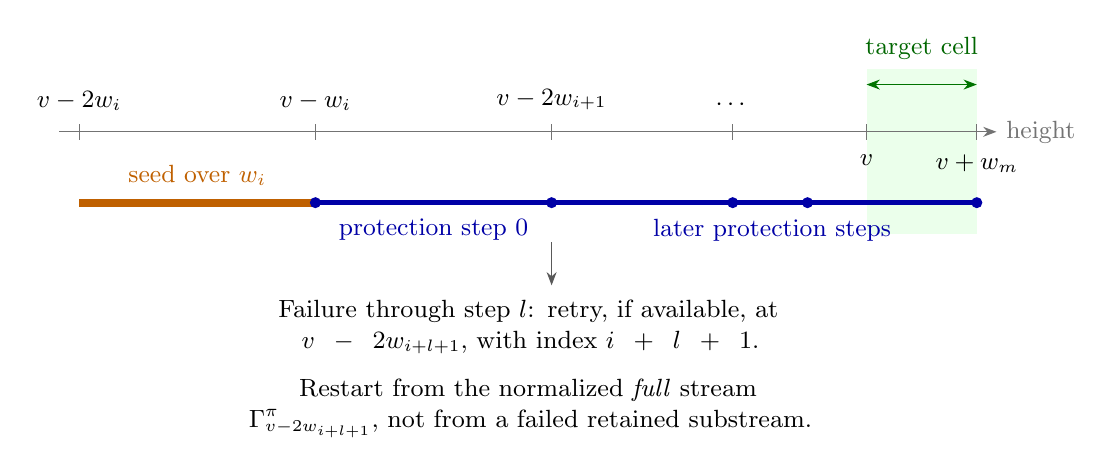
\begin{tikzpicture}[x=1cm,y=1cm,font=\small,>=Stealth]
  \fill[green!8] (10,-.4) rectangle (11.4,1.7);
  \node[anchor=south,text=green!40!black] at (10.7,1.7) {target cell};
  \draw[<->,green!45!black] (10,1.5) -- (11.4,1.5);
  \draw[->,black!55] (-.25,.9) -- (11.65,.9) node[right] {height};
  \foreach \x in {0,3,6,8.3,10,11.4}
    \draw[black!55] (\x,.8) -- (\x,1);
  \node[anchor=south] at (0,1.05) {$v-2w_i$};
  \node[anchor=south] at (3,1.05) {$v-w_i$};
  \node[anchor=south] at (6,1.05) {$v-2w_{i+1}$};
  \node[anchor=south] at (8.3,1.05) {$\cdots$};
  \node[anchor=north] at (10,.73) {$v$};
  \node[anchor=north] at (11.4,.73) {$v+w_m$};
  \draw[line width=3pt,orange!75!black] (0,0) -- (3,0);
  \node[anchor=south,text=orange!75!black] at (1.5,.1) {seed over $w_i$};
  \draw[line width=2pt,blue!65!black] (3,0) -- (11.4,0);
  \foreach \x in {3,6,8.3,9.25,11.4}
    \fill[blue!65!black] (\x,0) circle (2pt);
  \node[anchor=north,text=blue!65!black] at (4.5,-.08) {protection step $0$};
  \node[anchor=north,text=blue!65!black] at (8.8,-.08) {later protection steps};
  \draw[->,black!65] (6,-.5) -- (6,-1.05);
  \node[anchor=north,align=center,text width=11.8cm] at (5.7,-1.12)
    {Failure through step $l$: retry, if available, at\\
     $v-2w_{i+l+1}$, with index $i+l+1$.};
  \node[anchor=north,align=center,text width=11.8cm] at (5.7,-2.12)
    {Restart from the normalized \emph{full} stream
     $\Gamma_{v-2w_{i+l+1}}^{\pi}$, not from a failed retained substream.};
\end{tikzpicture}

\caption{The height schedule of one opportunity, not sample paths.
With $w_i=16^{-i}w_0$, seeding runs from $v-2w_i$ to $v-w_i$.
Nonfinal protection step $l$ ends at $v-2w_{i+l+1}$;
the final step ends at $v+w_m$ and covers the entire target cell.
A failed nonfinal protection consumes the traversed opportunities,
and any retry starts from the normalized full stream at its new base.
There is no retry after the final opportunity. The marked first
endpoint illustrates the geometric endpoint relation only. The initial
$\min(l_0,m-i)$ protection steps are tested together at their last
endpoint, so the diagram does not prescribe a retry at step zero.
Heights are not drawn to scale.}
\label{fig:nested-opportunities}
\end{figure}

\paragraph{Costs of the late protection steps.}
Set \(a'=2Ak\) and \(\lambda'=\lambda/4\). We will obtain,
conditionally at every active late step,
\[
\begin{aligned}
 E\big[e^{\lambda'(Z_l\wedge a'(l+1))}\mid\text{past}\big]
   &\le e^{C_{\rm mg}k},\\
 P(Z_l>a'(l+1)\mid\text{past})
   &\le e^{-(\lambda/2)a'(l+1)},
\end{aligned}
\tag{36}\label{eq:36}
\]
where \(C_{\rm mg}\) is independent of \(A\ge1\) and \(k\ge2\).
The cutoff \(l_0\), unlike \(C_{\rm mg}\), may depend on these
parameters, the seed constants, and fixed retry counts. The rapid-loss
estimate is uniform over normalized starting laws with the required
separation; it does not depend on the early retained mass \(g_1\).

Indeed, \eqref{eq:7} gives, for each fixed retry count \(L'\),
\[
 \frac{3w_i16^{-l}}{n(d_l/(2L'))}
 \le 3C_*\left(\frac{32L'}{c_0}\right)^2\left(\frac4{16}\right)^l
 =: C_{k,L'}e^{-\theta l},\qquad \theta=\log4.
\]
Choose a fixed \(c_x>0\) with
\((1+\lambda)c_x<\theta\) and \(c_x<1\). For
\(0\le x\le c_xl\), use \eqref{eq:32} with \(L'=1\).
After increasing \(l_0\), its second term is at most
\(e^{-\lambda x}\). Below the applicability threshold
\(k\log(1/\kappa)\), use the trivial bound one. Both ranges therefore
give
\[
 P(Z_l>x\mid\text{past})\le
 \min\{1,e^{C'k-\lambda x}\},\qquad 0\le x\le c_xl,
\]
with \(C'\) independent of \(A,k\).
For \(c_xl\le x\le a'(l+1)\), take a fixed integer
\(L'\) sufficiently large that
\(\theta L'>(1+2\lambda)a'\), and increase \(l_0\) again.
The same rapid-loss estimate then gives
\[
 P(Z_l>x\mid\text{past})
 \le 2^{L'}e^{CkL'-\lambda x}
       +(2CkC_{k,L'})^{L'}e^{x-\theta lL'}
 \le e^{-\lambda x/2}.
\]
Here \(l_0\) absorbs both the constants and the ellipticity threshold
for this fixed retry count. Also
\(a'(l+1)\le2Akm\le kb/4<B_*\).
Finally, integrating these tails with \(\lambda'=\lambda/4\) gives
\[
\begin{split}
 E[e^{\lambda'(Z_l\wedge a'(l+1))}\mid\text{past}]
 &\le 1+\lambda'\int_0^\infty e^{\lambda'x}
                  \min\{1,e^{C'k-\lambda x}\}\,dx
       +\lambda'\int_0^\infty e^{-\lambda x/4}\,dx\\
 &\le \frac43 e^{C'k/4}+1\le e^{C_{\rm mg}k}.
\end{split}
\]
This proves \eqref{eq:36} with the required uniformity.

\paragraph{Why all opportunities rarely fail.}
Now impose \(\lambda'A>C_{\rm mg}+8\). If the first cumulative
late failure occurs at \(l\), either \(Z_l>a'(l+1)\) or the
sum of the truncated costs exceeds \(Ak(l+1)\). Earlier passing
costs are below their own cutoffs, since they are nonnegative. Setting
inactive costs to zero, conditional iteration of \eqref{eq:36} bounds
the second event by
\[
 \exp\{C_{\rm mg}k(l-l_0+1)-\lambda'Ak(l+1)\}.
\]
Together with the cutoff tail, this is at most \(e^{-5k(l+1)}\).
A failed attempt consuming exactly \(n\) opportunities consequently
has probability at most \(e^{-2kn}\), measured at its start. The
possibilities are seed failure (\(n=1\)), early-protection failure
(\(n=\min(l_0,m-i)\)), and a first late failure (\(n=l+1\));
the stronger bounds just proved absorb any coincidence of these counts.

Each such failure is known before the next available opportunity, so
revealing the full stream up to the new start leaves its upper layers
fresh. Exhaustion partitions the \(m\) opportunities into positive
consumed blocks. For a specified composition of \(m\), conditional
iteration gives probability at most \(e^{-2km}\). There are
\(2^{m-1}\) compositions, so the probability that this cell has no
certificate is at most
\[
 e^{-(2k-\log2)m}.
\]

\paragraph{Choosing the constants.}
We can now choose constants in an order justified by the preceding
estimates. Fix \(C_{\rm mg}\), then take \(A\ge1\) with
\(\lambda'A>C_{\rm mg}+8\), and define
\[
 f=2+\Lambda j_*,\qquad \chi=g+1+\Lambda j_*.
\]
Choose \(g,K\) with
\(1/g<\beta/64\) and \((1+f/g)D_0/K<\beta/64\), and then choose
\(k\ge2\) so large that
\[
 \lambda k/4>2K+4,\qquad
 (2k-\log2)j_*>\chi+2+\Lambda j_*+2K+4.
 \tag{37}\label{eq:37}
\]
Next fix the seed constants and retry counts, choose \(l_0\) to
validate \eqref{eq:36}, and then obtain \(g_1\) from early clipping
with its specified error \(e^{-6kl_0}\). All these constants precede
\(b\). Thus even this very small early-protection error causes no
circularity: its possibly small retained mass \(g_1\) is fixed before
we enlarge \(b\). Finally enlarge \(s_{\rm fl}\), after \(b\), to
meet all scale and separation thresholds.

\paragraph{The full stream and the short heights.}
By \eqref{eq:31}, outside an event of probability at most
\(e^{-(2K+2)b}\) for sufficiently large \(b\),
\[
 \|\Gamma_h^\pi\|\ge q_\pi\ge e^{-B/4}\qquad\text{for every }h.
\]
We combine this exception with the cell failures by a union bound; none
of the cell-attempt estimates is conditioned on this full-stream event.

To cover heights up to \(H_e\), apply \eqref{eq:32} at horizon
\(H_e\), with \(d'=r_s/2\), \(x=B/2\), and a fixed retry count
\(L'>k/2+2K+4\). By \eqref{eq:7},
\[
 \frac{H_e}{n(d'/(2L'))}\le C(L')e^{-b}.
\]
Raising the rapid-loss bound to its indicated power gives an upper bound
of the form
\[
 C\bigl(e^{-\lambda kb/2}+e^{-(L'-k/2)b}\bigr)
 \le e^{-(2K+2)b}
\]
for large \(b\), by \eqref{eq:37}. Off this event, taking prefixes
gives mass at least \(e^{-B/2}\) at every height through \(H_e\)
with relative-motion budget \(r_s/2\). Initial separation is at least
\(r_s\), so these prefixes have separation at least
\(r_s/2\ge r_{s_-}\), again by \eqref{eq:7}.

\paragraph{Assembling the cell certificates.}
The total number of cells, including the separate growth cell, is at most
\[
 C\exp[(\chi+1+\Lambda j_*)b]+2
 \le\exp[(\chi+2+\Lambda j_*)b].
\]
On successful completion of the attempt from opportunity \(i\),
separation throughout that cell is at least \(c_0\rho_i/2\). The
scale inequality gives
\[
 n(c_0\rho_i/2)\ge\frac{c_0^2}{4C_*}w_i.
\]
For the traversal cells,
\[
 w_i\ge w_m\ge cse^{-(1+\Lambda j_*)b},
\]
which exceeds the required scale \(s_-=se^{-fb}\) after multiplication
by the preceding fixed constant. For the growth cell,
\[
 w_i\ge cse^{(\chi-\Lambda j_*)b},
\]
which similarly exceeds \(s_+=se^{gb}\). In each comparison the
remaining factor \(e^b\) absorbs the fixed constants for large \(b\).
Thus the certificate supplies the separation required in
\eqref{eq:35} at every height of its cell.

On the separately controlled event \(q_\pi\ge e^{-B/4}\), concatenate
the full stream to the attempt start with the restricted seed and
protection kernels. Their mass, and therefore their prefix mass at each
height of the cell, is at least
\[
 e^{-B/4}g_0g_1e^{-Akm}\ge e^{-B},
\]
because \(Akm\le B/8\) and \(g_0,g_1\) are fixed before \(b\).
The cell lies entirely in the protected part of the construction.

A union bound over cells, using \eqref{eq:37}, bounds the probability
of any missing cell certificate by \(e^{-(2K+2)b}\) for large \(b\).
Adding the full-stream and short-height exceptions proves
\eqref{eq:35}. At fixed \(b\), all the smallest scales tend uniformly
to infinity with \(s_{\rm fl}\). Enlarging that floor therefore
satisfies every scale and separation threshold used above.
\end{proof}

\subsection{Episode operation}

We now use the stage estimate to construct the actual episode boundaries.
Only the kernel tests in \eqref{eq:35} determine those boundaries; the
longer cell certificates in its proof do not enter the stopping rule.
Every retained measure below is a deterministic restriction of a kernel,
followed by normalization. No sample of a path is required.

\paragraph{Starting an episode.}
Start at height zero, and start a new episode after each reset below
\(N\). At an episode's initial height \(t<N\), take the global
normalized endpoint law
\[
 \mu_t=K_t(0,\cdot)/a_t
\]
in product \(k\) times. Inject this tuple law into layer \(t+1\)
with separation at least \(r_{s_{\rm fl}}\), using bounded elliptic
scripts. Concretely, choose \(k\) fixed positive integer offsets in
coordinate two, spaced by more than \(2r_{s_{\rm fl}}\). Prescribe
one particle's endpoint at a time, choosing the first offset whose
endpoint is at distance at least \(r_{s_{\rm fl}}\) in coordinate
two from every previously prescribed endpoint. Each earlier endpoint
excludes at most one of the \(k\) choices, so a choice always exists.
Move that particle laterally by its chosen offset and then directly up
one layer.

The scripts have a fixed length bound and hence cost at most a fixed
logarithmic mass \(B_0\). Normalize the retained tuple mass and set
\(s=s_{\rm fl}\). If the injection reaches \(N\), end the episode
there without a stage.

\paragraph{Testing one stage.}
At the current height \(u<N\), let \(\pi\) be the retained
normalized tuple law and let \(s\ge s_{\rm fl}\) be its scale.
Plan \(H=\lfloor se^{\chi b}\rfloor\) layers. Test the traversal
inequality in \eqref{eq:35} successively at offsets
\[
 h=1,\ldots,\min(H,N-u).
\]
Stop at the first failure. If offset \(H\) is reached, also test the
growth inequality there. All these tests use the same initial law
\(\pi\) and the full kernel from \(u\); passing an intermediate
test does not restrict the mass used for later tests.

\paragraph{Retaining mass and updating the scale.}
If the full planned stage passes, retain and normalize the growing
separated mass, and replace \(s\) by \(s_+=se^{gb}\).
If a test fails, replace \(s\) by \(s_-=se^{-fb}\) and retain mass
with the corresponding smaller separation. For a failed growth test,
the traversal test at the same height already supplies this mass. For
a first traversal failure at offset \(h\), extend the passing mass at
\(h-1\) by one direct upward step for every particle. At \(h=1\)
use the initial probability law as that passing mass. These upward
steps preserve separation, and in every failure case the retained mass
is at least
\[
 e^{-B}\kappa^k.
\]
Normalize it. If the updated scale is below \(s_{\rm fl}\), end the
episode and, if its endpoint is below \(N\), start the next episode
by the preceding injection rule. Otherwise continue with the next
stage at the new scale.

At height \(N\), end in all cases. A passing stage stopped at an
offset strictly less than \(H\) is called incomplete; its traversal
test supplies mass at least \(e^{-B}\). There is at most one such
stage. A failure encountered before this truncation still implies a
failure of the untruncated tests in \eqref{eq:35}, so it has the same
conditional probability bound under the fresh law \(P\).

Every test and retention uses only rows strictly below its actual
endpoint. Therefore all stage and episode boundaries are stopping times
for the layer filtration. In particular, the upper layers at every
subsequent stage start are fresh under \(P\).

Let \(J,F\) be the total numbers of stages and failed stages, and let
\(M\) be the number of episodes, with boundary heights
\(0=t_0<t_1<\cdots<t_M=N\). Put
\[
 h_i=t_{i+1}-t_i,\qquad
 J_i=\#\{\text{stages in episode }i\},\qquad
 c_i=\log(a_{t_i}/a_{t_{i+1}}),\qquad 0\le i<M.
\]

\begin{lemma}[Episode bounds]\label{stage-episodes}
For sufficiently large fixed \(b\), the episode construction satisfies
\(M\le J+1\) and
\[
 0\le c_i\le B_0/k+2bJ_i,\qquad
 \log(1+h_i)\le C(1+J_i).
 \tag{38}\label{eq:38}
\]
For large \(N\),
\[
 J\le\frac{\log N}{gb}+(1+f/g)F+1.
 \tag{39}\label{eq:39}
\]
Under \(Q_N\), fixed constants \(c,C>0\) and \(L_0<\infty\)
satisfy
\[
\begin{aligned}
 c\log N&\le E_{Q_N}M,& E_{Q_N}(M+J)&\le C\log N,\\
 E_{Q_N}\sum_{i<M}c_i\mathbf1_{\{J_i\le L_0\}}
   &\ge c\log N.&&
\end{aligned}
\tag{40}\label{eq:40}
\]
With the padding \(t_i=N\) for \(i\ge M\), each \(t_i\) is a
bounded layer stopping time, and \(\{i<M\}\) is known at \(t_i\).
\end{lemma}

\begin{proof}
\smallskip\noindent\textbf{Mass and height within an episode.}
The unrestricted quenched \(k\)-survival mass through \(t_i\) is
\(a_{t_i}^k\). Starting from its normalized endpoint law, our retained
continuation costs at most
\(B_0+(kb+k\log(1/\kappa))J_i\) in logarithmic mass. Its
concatenation is contained in the original survival kernel through
\(t_{i+1}\), so
\[
 a_{t_{i+1}}^k\ge a_{t_i}^k
 \exp\{-B_0-(kb+k\log(1/\kappa))J_i\}.
\]
This proves the upper bound for \(c_i\) in \eqref{eq:38} once
\(b\ge\log(1/\kappa)\); its nonnegativity follows from the
monotonicity of \(a_t\). Each stage length is at most
\(se^{\chi b}\), and the scale increases from the fixed floor by
at most a factor \(e^{gb}\) per stage. Summing these geometric
bounds, together with the one-layer injection, proves the height bound
in \eqref{eq:38}. Every episode except possibly the last contains a
failed stage, so \(M\le J+1\). The last episode may consist only of
its injection.

\smallskip\noindent\textbf{Counting stages by their scale changes.}
For this accounting only, update the scale after the last completed or
failed stage as if the operation continued, and clamp it upward to the
floor after a reset. Every completed success consumes its full planned
height \(H\ge s_+\), so its updated scale is at most
\(\max(s_{\rm fl},N)\). Failures decrease the scale, and the
clamping returns it only to \(s_{\rm fl}\). If \(S\) is the
number of completed successes, their increases of \(gb\), minus the
losses of at most \(fb\) per failure, therefore satisfy
\[
 gbS-fbF\le\log(N/s_{\rm fl})\le\log N
\]
for large \(N\). There is at most one passing incomplete stage, so
\(J\le S+F+1\). This proves \eqref{eq:39}.

\smallskip\noindent\textbf{Transferring the failure bound to \(Q_N\).}
Under \(P\), conditional on the past at any actual stage start, its
failure probability is at most \(e^{-2Kb}\). If \(I\) is its
failure indicator, then
\[
\begin{split}
 E_P[e^{KbI-e^{-Kb}}\mid\text{stage past}]
 &\le e^{-e^{-Kb}}
       \bigl(1+e^{-2Kb}(e^{Kb}-1)\bigr)\le1.
\end{split}
\]
There are at most \(N\) actual stages, since every stage advances at
least one layer. Pad the list to \(N\) slots, with active indicator
\(A_r\), and put \(I_r=0\) in inactive slots. Before each slot its
activity is known, and
\[
 E_P\big[e^{KbI_r-e^{-Kb}A_r}\mid\text{past}\big]\le1.
\]
The inactive factor is one. Conditional iteration, using
\(\sum_r I_r=F\) and \(\sum_r A_r=J\), gives
\[
 E_P e^{KbF-e^{-Kb}J}\le1.
\]
Applying the entropy inequality with \eqref{eq:34} yields
\[
 KbE_{Q_N}F\le D_0\log N+e^{-Kb}E_{Q_N}J.
\]
Only the exponential estimate was taken under the fresh law; this last
inequality requires no independence under \(Q_N\).

Write \(c_f=1+f/g\). Combining the last inequality with
\eqref{eq:39} gives
\[
 E_{Q_N}J\le
 \frac{\log N}{b}\left(\frac1g+\frac{c_fD_0}{K}\right)
 +\frac{c_fe^{-Kb}}{Kb}E_{Q_N}J+1.
\]
The coefficient in parentheses is less than \(\beta/32\). After
absorbing the exponentially small term, for large fixed \(b\) and
then large \(N\),
\[
 2bE_{Q_N}J\le\frac\beta4\log N.
\]

\smallskip\noindent\textbf{Positive loss in episodes with bounded stage count.}
Under \(Q_N\),
\(\sum_{i<M}c_i=-\log a_N>\beta\log N\). Summing
\eqref{eq:38} and using the last bound shows
\[
 \frac{B_0}{k}E_{Q_N}M
 \ge\beta\log N-2bE_{Q_N}J
 \ge\frac{3\beta}{4}\log N.
\]
This proves the lower bound on \(E_{Q_N}M\); its upper bound, together
with that on \(E_{Q_N}J\), follows from \(M\le J+1\).
For any \(L_0>0\), the loss in the remaining episodes satisfies
\[
 \sum_{i<M}c_i\mathbf1_{\{J_i>L_0\}}
 \le\left(\frac{B_0}{kL_0}+2b\right)J.
\]
Although the injection cost \(B_0\) may be large, it is fixed. Choose
\(L_0\) after it so that the first term's expected contribution is
at most \((\beta/4)\log N\). Episodes with more than \(L_0\)
stages then account for at most \((\beta/2)\log N\) of expected
loss. Subtracting this from the total proves the last assertion of
\eqref{eq:40}.

Finally, the operational tests use only rows below their tested layer,
so all episode boundaries are bounded layer stopping times. With the
stated padding, \(\{i<M\}=\{t_i<N\}\) is known at \(t_i\).
\end{proof}

\section{Stationary profiles and the contradiction}\label{sec:stationary}

We retain the bad-event laws \(Q_N\) and the adapted episodes from
Section~\ref{sec:stages}. Their entropy and drop bounds
\eqref{eq:34}, \eqref{eq:38}, and \eqref{eq:40} will produce a stationary
sequence of local endpoint profiles with positive mean normalization
loss. We begin by identifying the statistic that will make this
stationary law impossible.

For a full-support subprobability \(w\) on horizontal space, define
\[
 T_R(w)=\max_{j\in\mathbb Z}
       \min\{w(z_2\le j),w(z_2\ge j+R)\},\qquad R\in\mathbb Z_{\ge1}.
\]
Here \(z_2\) denotes the second full-space coordinate. This positive,
translation-invariant quantity measures how much mass can be placed in
each of two tails separated by \(R\). The profile update multiplies
surviving mass by the episode normalization factors. The outward-order
estimate~\eqref{eq:33} transports the two tails at a cost logarithmic
in the traversed height, together with a local environmental remainder.
For a stationary marked profile law, we will derive
\[
 mE c_0\le A_\to E\log\left(1+\sum_{i=0}^{m-1}h_i\right)+O(1),
\]
with the last term independent of \(m\). The logarithmic height moment
from the episode bounds makes the right side \(o(m)\), contradicting
\(E c_0>0\).

The construction must supply a profile to which this argument applies.
Local limits can initially have diffuse mass or several components
escaping from one another. The array below retains those possibilities,
then finite-window entropy excludes diffuse mass and reduces the
positive-loss event to finitely many persistent components of full
support. Marking one component uniformly preserves stationarity. The
same entropy bound controls its upper environment relative to an iid
field while retaining exactly its current profile and offset data.

Translation-invariant compactifications that retain separated components
and diffuse mass were developed by Mukherjee and
Varadhan~\cite[Theorem~3.2]{MukherjeeVaradhan2016} for occupation measures
and by Bates and Chatterjee~\cite[Theorem~2.8]{BatesChatterjee2020} for
polymer endpoint distributions. We construct the array needed here
directly, storing sampled-anchor offsets together with episode marks
and the corresponding upper environments.

To remove the environmental bias from the local remainder, we first fix
a finite number \(m\) of episodes and send the tail separation \(R\)
to infinity. Only afterwards do we send \(m\) to infinity. No mixing
estimate uniform in the episode window is needed. The final profile
argument establishes the displayed obstruction in this order.

\subsection{The stationary array}


Horizontal space is \(\mathbb Z^{d-1}\). We observe profiles from sampled
anchors, allowing offsets between anchors to escape to infinity in the
limit.

Pad each episode sequence to all integer indices by \(t_i=0\) for \(i<0\), \(t_i=N\) for \(i\ge M\), and zero marks \(h_i,J_i,c_i\) outside \(0\le i<M\). Write \(\mu_i^*=\mu_{t_i}\) for the normalized global endpoint profile there, viewed as a probability on horizontal sites. Conditional on the entire environment, sample anchors \(U_{i,a}\sim\mu_i^*\) independently for indices \(i\in\mathbb Z\) and \(a\ge1\). Keep the following array in a countable compact product:
\begin{itemize}
\item The nonnegative integer marks \(h_i,J_i\) and nonnegative real marks
\(c_i\), each range compactified by \(+\infty\).
\item The offsets \(O_{ia,jb}=U_{j,b}-U_{i,a}\), in the lattice with its
one-point compactification, and all profile coordinates
\(w_j^{ia}(z)=\mu_j^*(U_{i,a}+z)\).
\item The upper environments \(\Omega^{i,m,a}(l,z)\), for \(m\ge1\),
\(l\ge0\), and horizontal \(z\). For \(l<t_{i+m}-t_i\), use the true row
\(\omega((t_i+l,U_{i,a}+z),\cdot)\). At the remaining heights use the
row at \((l,U_{i,a}+z)\) of a full auxiliary iid upper field for the
pair \((i,m)\). This field is common to all anchors \(a\), and the
auxiliary fields are independent across pairs and independent of the
environment and anchors.
\end{itemize}
Denote by \(P_\uparrow\) the iid upper-field law on indices \((l,z)\),
including \(l=0\). The functions \(q(0;\Omega)\) and
\(a_H(0;\Omega)\) are the earlier quenched no-drop functions evaluated
in this upper field; they require no rows below its base.

Profile and row coordinates use the ordinary compact ranges \([0,1]\) and the row simplex, respectively. Let \(\tau\) shift the array by reading all absolute episode indices one index later (leaving relative offsets in time such as \(m\) unchanged). Take the probability law \(\mathbb L_N\) averaging shifts to episode starts:
\[
\mathbb L_N[F]=(E_{Q_N}M)^{-1} E_{Q_N,{\rm aux}}\sum_{i=0}^{M-1}F(\tau^i{\rm array}) .
\]
\begin{lemma}[Stationary episode limit]\label{profile-stationary}
Along a subsequence, \(\mathbb L_N\) converges weakly to a shift-invariant
law \(\mathbb L\). Under this law, simultaneously for every \(i\),
\[
\begin{gathered}
1\le h_i<\infty,\qquad J_i,c_i<\infty,\\
E_{\mathbb L}\bigl(c_i+\log(1+h_i)\bigr)<\infty,
\qquad E_{\mathbb L}c_i>0.
\end{gathered}
\]
Every stored row is uniformly elliptic with the original bound
\(\kappa\).
\end{lemma}

\begin{proof}
Compactness gives a subsequential weak limit. The shift is continuous,
and the occupation sum telescopes: for every bounded continuous \(F\),
\[
\left|\mathbb L_N[F\circ\tau]-\mathbb L_N[F]\right|
\le \frac{2\|F\|_\infty}{E_{Q_N}M}\longrightarrow0.
\]
At the origin, \eqref{eq:40} bounds the occupation mean of \(J_i\).
Truncation passes this bound to the limit, so \(J_0<\infty\) almost
surely. The bounds \eqref{eq:38} then pass and give the stated
integrability and finiteness. For the positive truncated-drop bound in
\eqref{eq:40}, put $C_{L_0}=B_0/k+2bL_0$ and use the globally
bounded continuous test
\[
 (c_0\wedge C_{L_0})\mathbf1_{\{J_0\le L_0\}}.
\]
It agrees with the required drop on every supported array, by
\eqref{eq:38}. Its expectation therefore passes to the limit and gives
$E_{\mathbb L}c_0>0$. The occupation law gives \(h_0\ge1\),
and shift invariance gives all assertions at every integer index.
Uniform ellipticity is a closed condition on the row coordinates and
therefore also passes to the limit.
\end{proof}

Write
\[
H_{i,m}=\sum_{s=i}^{i+m-1}h_s,\qquad C_{i,m}=\sum_{s=i}^{i+m-1}c_s .
\]
By the stationary ergodic theorem, in its possibly nonergodic form
\cite[Theorem~6.2.1]{Durrett2019}, there exists \(\zeta>0\) and a
shift-invariant positive-probability event
\[
\mathcal E=\{\lim_{m\to\infty}C_{0,m}/m>\zeta\}
\tag{41}\label{eq:41}
\]
(up to null sets).

\subsection{Entropy in a finite episode window}

We use standard relative-entropy tools originating with Kullback and
Leibler~\cite{KullbackLeibler1951}; the binary-event and projection
inequalities are instances of data processing, as discussed in
Sason and Verd\'u~\cite[Section~II-B]{SasonVerdu2016}. Their needed forms,
including the variational formula, are proved below before being applied
to the stopped episode windows.

Current data for entropy purposes are only
\[
\mathcal A_i=\big((O_{ia,ib})_{a,b},(w_i^{ia}(z))_{a,z}\big).
\]
The reference law keeps the marginal of \(\mathcal A_i\).
Conditionally on these data, labels at finite offsets share one iid
upper field, translated by their offsets, while distinct classes use
independent iid fields. The finite-offset relations in the limit are
consistent equivalence relations with additive offsets: each specified
finite-offset event is clopen, so every such consistency identity passes
to the limit. Write \(\mathbf R(\mathcal A_i,d\phi)\) for this reference
conditional field law.

\begin{lemma}[Finite-window entropy]\label{profile-entropy}
There is a constant \(C_E<\infty\) such that, for every fixed \(i\) and
\(m\ge1\), the \(\mathbb L\)-law of
\((\mathcal A_i,(\Omega^{i,m,a})_a)\) has relative entropy at most
\(C_E m\) with respect to its own current-data marginal followed by
the reference kernel \(\mathbf R\).
\end{lemma}

\begin{proof}
We first record the elementary entropy facts used here. Relative
entropy is \({\rm KL}(Q\mid P')=\int f_0\log f_0\,dP'\), where
\(f_0=dQ/dP'\), and is infinite without absolute continuity. It has
the variational formula
\[
{\rm KL}(Q\mid P')
=\sup_{F\text{ bounded measurable}}
\left\{QF-\log P'e^F\right\}.
\]
The upper bound follows from Jensen applied to \(e^F/f_0\).
For equality, truncate \(\log f_0\) between \(\pm B\) and send
\(B\to\infty\), or test a singular set. Thus projection cannot
increase entropy. On compact metric spaces, bounded continuous tests
suffice by bounded approximation in \(L^1(Q+P')\); the variational
formula therefore gives lower semicontinuity under joint weak
convergence of both laws.

For an event of respective probabilities \(s,t\), where \(0<t<1\),
projection to its indicator gives
\({\rm KL}(Q\mid P')\ge s\log(1/t)-\log2\).
If a reference law is a data marginal times an independent fixed law,
replacing that marginal by the controlled law's \emph{own} data
marginal only decreases finite entropy. Indeed the new density is
the old density divided by its conditional mean given the data, and
the entropy difference is the nonnegative marginal entropy. These
log-density identities are taken on sets of positive controlled
density; negative parts are integrable, and conditional Jensen for
\(f_0\log f_0\) justifies the marginal term.

Before the limit, at deterministic \(i\ge0\), put
\(\mathcal H_i=\sigma(\mathcal F_{t_i},(U_{i,a})_a)\) and
\(\Phi_i=(\Omega^{i,m,a})_a\); \(\mathcal A_i\) is
\(\mathcal H_i\)-measurable. Include the same auxiliary sampling under
\(P\). Given \(\mathcal H_i\), the spliced field above \(t_i\), in
absolute horizontal coordinates, is still iid under \(P\). Indeed, at
both bounded layer stopping times the layers at and above the stopping
layer are fresh, while the current anchors use only lower-layer data.
Keeping the slab up to the second stopping layer and replacing its tail
by an independent copy therefore preserves the iid law. Thus \(\Phi_i\)
has conditional law \(\mathbf R(\mathcal A_i,d\phi)\).

Let \(L_t=dQ_N|_{\mathcal F_t}/dP|_{\mathcal F_t}\). Under \(Q_N\),
the conditional density of the information stopped at \(t_{i+m}\),
together with the independent extension, relative to the corresponding
\(P\)-law given \(\mathcal H_i\), is \(L_{t_{i+m}}/L_{t_i}\).
The anchors at \(i\) use the same lower-data sampling kernel under both
laws, and the extension costs no density. Conditional Jensen therefore
gives, for every bounded \(F\),
\[
\begin{aligned}
&E_{Q_N,{\rm aux}}[F(\mathcal A_i,\Phi_i)\mid\mathcal H_i]\\
&\quad\le
E_{Q_N,{\rm aux}}[\log L_{t_{i+m}}-\log L_{t_i}\mid\mathcal H_i]
+\log\int e^{F(\mathcal A_i,\phi)}\mathbf R(\mathcal A_i,d\phi).
\end{aligned}
\]
Multiply by \(\mathbf1_{\{i<M\}}\), which is past-known, and average as for \(\mathbb L_N\). Jensen to pull the log outside this average gives the \(\mathbb L_N\) entropy bound at index zero (against its own current-data marginal and the kernel) of
\[
\frac{1}{E_{Q_N}M}\sum_{i\ge0}E_{Q_N}\big[\log L_{t_{i+m}}-\log L_{t_i}\big]
\le \frac{mD_0\log N}{E_{Q_N}M}.
\]
Increments from \(i\ge M\) are zero. The displayed sum telescopes
over deterministic indices, since \(t_i=N\) for \(i\ge N\); its
subtracted initial expected log densities are nonnegative relative
entropies. For passage to the limit, finite-class consistency is a
closed condition: self-offsets vanish, finite offsets are symmetric
with sign change, and specified finite offsets add on triples.
Violations are detected by finitely many clopen coordinate events.
On this support the reference kernel is weakly continuous. For any
finitely many field coordinates, coincidence of the input sites is
specified by a finite-offset equality, while different sites have
independent rows. Finite-coordinate tests suffice by compactness.
Consequently the reference laws converge weakly with their current-data
marginals. Lower semicontinuity and \eqref{eq:40} yield the bound
\(C_E m\); shift invariance gives every \(i\).
\end{proof}

\subsection{Profiles and multiplicities}

Offsets across all times determine equivalence classes of labels
\((i,a)\) by finite distance. Within one class, the profiles at any
time \(j\), viewed from its different anchors, are translates of one
another and have total mass at most one. These consistency statements
pass coordinatewise.

\begin{lemma}[Sampling identities]\label{profile-sampling}
Under \(\mathbb L\), simultaneously for all indices and horizontal
\(z\),
\[
2^{-n}\sum_{b\le2^n}\mathbf1_{\{O_{ia,jb}=z\}}\longrightarrow w_j^{ia}(z)\quad\text{a.s.}
\tag{42}\label{eq:42}
\]
A distinct label \((j,b)\ne(i,a)\) cannot have finite offset \(z\)
from \((i,a)\) while \(w_j^{ia}(z)=0\).
\end{lemma}

\begin{proof}
Before the limit, the anchor draws at \(j\), excluding a possible
own label, are conditionally independent samples given the environment
and \(U_{i,a}\). The occupation indices and weights depend only on
the environment, not on these draws. The mean-square error in
\eqref{eq:42} is therefore \(O(2^{-n})\), including the possible
own-label contribution. The finite-offset indicators are continuous,
so these summable bounds pass to the limit. Borel--Cantelli proves
\eqref{eq:42}.

For distinct labels and any continuous function \(g\) on \([0,1]\),
the same conditional sampling identity gives
\[
E_{\mathbb L}\!\left[
g(w_j^{ia}(z))
\bigl(\mathbf1_{\{O_{ia,jb}=z\}}-w_j^{ia}(z)\bigr)\right]=0.
\]
Approximate the indicator of zero by bounded continuous functions
to obtain the second assertion. All the indices and sites are
countable, so the assertions hold on one common probability-one event.
\end{proof}

\begin{lemma}[Profile updates and averaged survival]\label{profile-updates}
For every \(i,m,a\), write \(H=H_{i,m}\), \(C=C_{i,m}\), and
\(\Omega=\Omega^{i,m,a}\). Coordinatewise,
\[
w_{i+m}^{ia}\ \ge\ e^C\, w_i^{ia} K_H^\Omega .
\tag{43}\label{eq:43}
\]
Here the kernel maps horizontal starting positions at layer zero to
endpoints at layer \(H\) in the anchor frame. Also, almost surely,
\[
\limsup_n 2^{-n}\sum_{a\le2^n} a_{H_{i,m}}(0;\Omega^{i,m,a})\le e^{-C_{i,m}}.
\tag{44}\label{eq:44}
\]
\end{lemma}

\begin{proof}
Before the limit, local no-drop continuation is contained in the global
survival stream. Dividing its endpoint inequality by the new global
mass gives \eqref{eq:43}, with
\(C=\log(a_{t_i}/a_{t_{i+m}})\). At finite limiting marks, pass first
the inequalities involving finitely many starting sites and
bounded-length successful kernel paths. Strict violations of these
finite-path inequalities are open, since each path weight is a finite
product of row coordinates. Increasing the finite restrictions gives
\eqref{eq:43}. Successful paths to layer \(H\) use no departure row
at or above \(H\), so the auxiliary tail is irrelevant.

Before the limit, at a fixed index the average in \eqref{eq:44} has
conditional mean at most \(e^{-C}\) given the environment, again by
the global mass inequality. Its terms are independent bounded
functions of the independently sampled current anchors; they do not
use appended rows. Chebyshev bounds the conditional probability of
exceeding \(e^{-C}+\epsilon\) by \(2^{-n}\epsilon^{-2}\), and this
also holds after occupation averaging. For fixed finite \(H\), the
function \(a_H\) is lower semicontinuous, being a sum of nonnegative
continuous finite-path weights. Thus the strict upper-violation event
is open at finite marks, and the same summable probability bound
passes to the limit. Borel--Cantelli, followed by a countable sequence
\(\epsilon\downarrow0\), proves \eqref{eq:44}.
\end{proof}

Call a current label \emph{proper} if \(w_i^{ia}(0)>0\), and
\emph{dust} otherwise.

\begin{proposition}[Finitely many persistent profiles]\label{profile-classes}
On \(\mathcal E\), there is no dust. The proper classes form the same
finite nonempty set at every time, and the profile of each class has
full support on horizontal space.
\end{proposition}

\begin{proof}
\emph{Dust is isolated.}
If a dust label \((i,a)\) had a distinct finite-offset neighbor
\((j,b)\), with offset \(z\), profile consistency would give
\(w_i^{jb}(-z)=w_i^{ia}(0)=0\). Apply the second assertion of
Lemma~\ref{profile-sampling} with \((j,b)\) as the reference label
and \((i,a)\) as the sampled target. This is impossible. Thus dust
labels are singleton classes even when all times are included.

At any fixed time, the dust indicators are exchangeable, because
anchor-permutation symmetry passes to the limit. They have an
asymptotic frequency \(\delta_i\), which is positive if any dust occurs. To see
the latter assertion, apply the ergodic theorem to the stationary
label sequence of dust indicators. On the invariant zero-frequency
event, taking expectations shows that each indicator vanishes.

Fix \(i,m\). Under the reference law of Lemma~\ref{profile-entropy},
conditional on \(\mathcal A_i\), the singleton dust classes have
independent upper fields. Their values \(q(0;\Omega^{i,m,a})\) are
therefore iid with mean \(p\). Finite entropy gives absolute
continuity, so the strong law on the dust subsequence also holds under
\(\mathbb L\) whenever that subsequence is infinite. Since
\(a_H\ge q\), including in every spliced field, \eqref{eq:44} yields
\[
e^{-C_{i,m}}\ge p\delta_i.
\]
This holds simultaneously for every \(m\). On \(\mathcal E\), its
left side tends to zero, by \eqref{eq:41} and stationarity. Dust is
therefore absent at all times on \(\mathcal E\).

\emph{There are finitely many proper classes.}
For fixed \(n\) and \(r_0>0\), whenever possible choose from
\(\mathcal A_i\) labels in \(n\) distinct classes with self masses
at least \(r_0\). On this selection event, when
\(C_{i,m}>\zeta m\), \eqref{eq:43} and the total-mass bound for
each output profile give
\[
\prod_{\rm chosen} q(0;\Omega^{i,m,a})\le r_0^{-n}e^{-n\zeta m}.
\]
The event of successful selection together with this deterministic
product bound is measurable from the current data and the extension
fields. Its reference probability is at most
\[
r_0^{-n\lambda}(E q^{-\lambda})^n e^{-\lambda n\zeta m},
\]
by \eqref{eq:4} and class independence. The binary entropy bound and
Lemma~\ref{profile-entropy} show that its \(\mathbb L\)-probability
has \(\limsup_{m\to\infty}\) at most \(C_E/(\lambda n\zeta)\).
On the selection event intersected with \(\mathcal E\), the product
bound holds for all sufficiently large \(m\). This bounds the
probability of that intersection by the same quantity. Send
\(r_0\downarrow0\), then \(n\to\infty\), to exclude infinitely
many proper classes.

\emph{The classes persist and have full support.}
Over any positive integer height, the local kernel has positive weight
between any two horizontal sites: move horizontally at the starting
layer and then ascend directly. Uniform ellipticity makes this finite
script positive. Thus \eqref{eq:43} gives a full-support next profile
for every current proper class. By \eqref{eq:42}, every positive
coordinate is represented by next-time labels. Distinct classes cannot
merge, by the global finite-offset equivalence relation.

Conditional on the shift-invariant event \(\mathcal E\), the current
number of classes is therefore nondecreasing, finite, positive, and
stationary. It is consequently constant almost surely. Indeed, writing $N_i$ for
this count, stationarity and monotonicity give
\[
 E[\min(N_{i+1},K)-\min(N_i,K)]=0
\]
for every integer $K$. The nonnegative difference vanishes almost
surely; letting $K$ increase proves $N_{i+1}=N_i$. This uses no moment
of the number of classes. The class sets transport bijectively
through time, and every profile has full support by the update from
the preceding time.
\end{proof}

\subsection{Why a stationary profile cannot sustain normalization growth}

The preceding construction has left us with a finite, persistent set of
full-support profiles on the event $\mathcal E$. Condition on
$\mathcal E$, mark one class uniformly, and use its least current label
as the origin at each episode. Uniform
marking commutes with time shift, so the marked law $\mathbb L_*$ is
stationary. This choice matters: a class sampled according to its mass
would generally receive a different weight after an episode.

For any fixed window of $m$ episodes, put
\[
 H_m=\sum_{i=0}^{m-1}h_i,\qquad C_m=\sum_{i=0}^{m-1}c_i.
\]
Write $w_0$ for the marked profile at the start of this window and write
$w_m$ in the same horizontal frame. Both are subprobability measures of
full support. The profile update gives
\[
 w_m\ge e^{C_m}w_0 K_{H_m}^{\Omega_m}
 \quad\hbox{coordinatewise},
\]
where $\Omega_m$ is the spliced upper field viewed from the current
representative. The profile at time $m$, with its usual representative,
has the same distribution as $w_0$ up to translation.

There is one further property of this marked field that we will need.
Let $D_*=(\mathcal A_0,a)$, where $\mathcal A_0$ is exactly the
current offset and profile data defined above and $a$ is the least
current label of the marked class. In particular, $D_*$ contains no
future episode marks or future profiles, and $w_0$ is a function of
$D_*$. The joint law of $(D_*,\Omega_m)$ has finite relative entropy with respect to
\begin{equation*}\tag{45}\label{eq:45}
 \mathbb L_*(D_*)\otimes P_\uparrow.
\end{equation*}
Indeed, conditioning on $\mathcal E$ changes the density of the projected
unmarked law by a factor at most $1/\mathbb L(\mathcal E)$. Finite entropy
therefore remains finite. Given the current data, uniform selection
among the current class representatives is a probability kernel. Apply
that same kernel to the reference law in Lemma~\ref{profile-entropy};
the selected field has iid law $P_\uparrow$ independently of the selected
index and the current data. Projection and the entropy chain rule now
give \eqref{eq:45} with the controlled law's own data
marginal.

The following argument isolates the remaining obstruction. It requires
finite entropy separately for each fixed $m$; no entropy bound uniform
in $m$ is used.

\begin{proposition}[No positive stationary normalization rate]
\label{profile-no-growth}
Suppose a stationary marked profile law has full-support subprobability
profiles and nonnegative marks $c_i$, positive integer marks $h_i$, with
\[
 E[c_0+\log(1+h_0)]<\infty.
\]
Assume the coordinatewise update \eqref{eq:43}, the finite
entropy property \eqref{eq:45} for every fixed $m$, and
the outward-order estimate \eqref{eq:33}, including its uniform local
approximation property. Then $Ec_0=0$.
\end{proposition}

\begin{proof}
We use the two-tail statistic introduced at the start of this section.
For an integer $R\ge1$, recall that
\[
 T_R(w)=\max_{j\in\mathbb Z}
 \min\{w(z_2\le j),w(z_2\ge j+R)\}.
\]
Here $z_2$ means the second full-space coordinate of a horizontal site.
Full support and finite mass imply $0<T_R(w)\le1$, and a maximizing
integer $j_R$ exists. Choose one measurably. For each fixed full-support
$w$, its maximizing cuts satisfy
\[
 j_R\longrightarrow-\infty,\qquad j_R+R\longrightarrow+\infty.
\]
For example, if $j_R$ were bounded below along a subsequence, the left
mass at both $j_R$ and $j_R-1$ would stay bounded below whereas the right
mass would tend to zero. Moving the cut one unit left would strictly
increase the smaller mass, contradicting maximality. The other endpoint
is treated by moving the cut right. Thus the normalized restrictions
$\alpha_-$ and $\alpha_+$ of $w_0$ to these two tails eventually sample
sites outside every fixed neighborhood of the representative origin.

Fix $m$ throughout the next steps. Let $Q_R$ be the mass of endpoint
pairs $(u,v)$ with $v_2-u_2\ge R$ under
\[
 (\alpha_-K_{H_m}^{\Omega_m})\otimes
 (\alpha_+K_{H_m}^{\Omega_m}).
\]
Every starting pair already has signed gap at least $R$. Its outward
order event is therefore contained in the event just tested. Finite
entropy transfers the probability-one event in \eqref{eq:33} to
$\Omega_m$, simultaneously for the countably many starting pairs and
integer heights, so it applies at the random height $H_m$. That estimate
and Jensen's inequality yield
\begin{equation*}\tag{46}\label{eq:46}
\begin{aligned}
 \log Q_R&\ge-A_\to\log(1+H_m)-Z_R,\\
 Z_R&=\iint\mathcal Z((0,x),(0,y);\Omega_m)
                \,\alpha_-(dx)\alpha_+(dy).
\end{aligned}
\end{equation*}
Write $\nu_\pm=\alpha_\pm K_{H_m}^{\Omega_m}$. There is an integer
$j$ with $\nu_-(u_2\le j)\ge Q_R/2$ and
$\nu_+(v_2\ge j+R)\ge Q_R/2$. Choose $j$ minimal for the first
inequality, so $\nu_-(u_2<j)<Q_R/2$. If the second inequality failed,
split ordered pairs into $u_2<j$ and $u_2\ge j$. The latter condition
forces $v_2\ge j+R$. Each part would then have mass strictly less than
$Q_R/2$, since both endpoint measures have mass at most one, contrary
to the definition of $Q_R$.

Each initial tail has mass at least $T_R(w_0)$. Applying
\eqref{eq:43} to the two tails at this cut gives
\begin{equation*}\tag{47}\label{eq:47}
 \log T_R(w_m)-\log T_R(w_0)
 \ge C_m-A_\to\log(1+H_m)-Z_R-\log2.
\end{equation*}
This is the decisive inequality: normalization contributes $C_m$,
whereas preserving the order of the two tails costs only a logarithm
of the traversed height and the local environmental remainder.

We next remove the environmental bias from that remainder. We claim
\begin{equation*}\tag{48}\label{eq:48}
 \limsup_{R\to\infty}E Z_R
 \le M_\mathcal Z:=\sup_{x,y}E_P\mathcal Z(x,y)<\infty.
\end{equation*}
Write $f_m(D,\Omega)$ for the density relative to
\eqref{eq:45}. Under that product reference, additionally
sample $x,y$ from $\alpha_-\otimes\alpha_+$ conditionally on $D$ alone.
Then $EZ_R$ is the reference expectation of
$f_m(D,\Omega)\mathcal Z((0,x),(0,y);\Omega)$.

The exponential moment in \eqref{eq:33} is uniform in the sampled pair.
Consequently the density and the remainder can both be truncated with
errors uniform in $R$. To see the only delicate part, on $\{f_m>B\}$
Young's inequality gives, for sufficiently small $\lambda>0$,
\[
 \lambda f_m\mathcal Z\le f_m\log f_m+e^{\lambda\mathcal Z}.
\]
The entropy term has vanishing tail. The reference probability of
$\{f_m>B\}$ is at most $1/B$, and Cauchy--Schwarz bounds the exponential
term on that event by $O(B^{-1/2})$. Once $f_m$ is bounded, truncating
$\mathcal Z$ is justified directly by its exponential moment.

Approximate the bounded density by a bounded nonnegative function
$g(D,\Omega)$ using only a fixed finite box of field rows around the
origin, allowing arbitrary dependence on $D$. With $L^1$ error at most
$\varepsilon$, its reference integral is at most $1+\varepsilon$.
Approximate the capped remainder, uniformly in $x,y$, by a bounded
function using fixed-radius
upper-row neighborhoods of those two sites. This follows from the
local approximation in \eqref{eq:33}; boundedness converts convergence
in probability to convergence in $L^1$. As $R$ increases, the two tail
supports and their neighborhoods leave the fixed origin box. Under the
product reference, conditional on $D,x,y$, the two approximating
factors then use disjoint iid row sets. Their product expectation is
bounded by $(M_\mathcal Z+\varepsilon)E_{P_\uparrow}g(D,\cdot)$.
The threshold in $R$ may depend on $D$; boundedness permits integration
by reverse Fatou. Sending the approximation errors to zero and removing
the truncations proves \eqref{eq:48}. This entire step
keeps $m$ fixed, so its approximation boxes need not be uniform in $m$.

\begin{figure}[tbp]
\centering
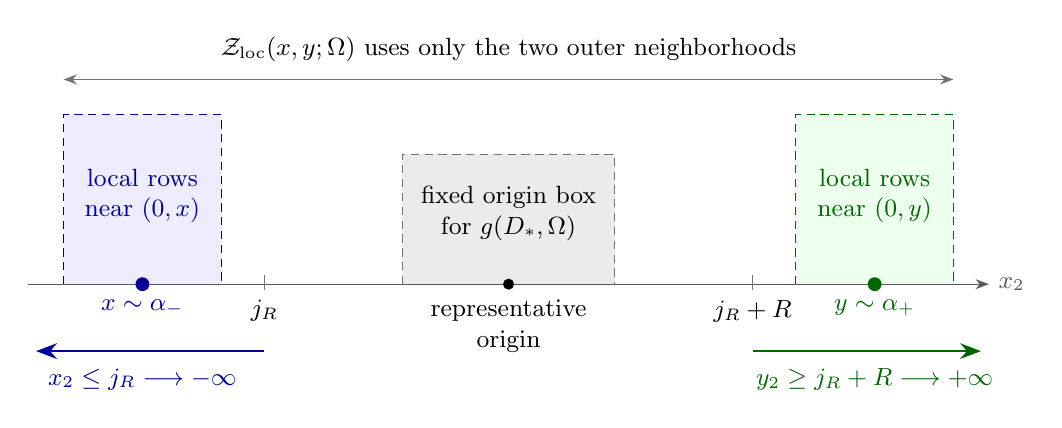
\begin{tikzpicture}[x=1cm,y=1cm,font=\small,>=Stealth]
  \fill[blue!7] (-5.65,0) rectangle (-3.65,2.15);
  \fill[green!7] (3.65,0) rectangle (5.65,2.15);
  \fill[black!8] (-1.35,0) rectangle (1.35,1.65);
  \draw[blue!60!black,densely dashed] (-5.65,0) rectangle (-3.65,2.15);
  \draw[green!40!black,densely dashed] (3.65,0) rectangle (5.65,2.15);
  \draw[black!55,densely dashed] (-1.35,0) rectangle (1.35,1.65);
  \node[align=center,text=blue!60!black] at (-4.65,1.12)
    {local rows\\near $(0,x)$};
  \node[align=center] at (0,.9) {fixed origin box\\for $g(D_*,\Omega)$};
  \node[align=center,text=green!40!black] at (4.65,1.12)
    {local rows\\near $(0,y)$};
  \draw[->,black!65] (-6.1,0) -- (6.1,0) node[right] {$x_2$};
  \fill (0,0) circle (2pt);
  \node[anchor=north,align=center] at (0,-.08) {representative\\origin};
  \fill[blue!60!black] (-4.65,0) circle (2.5pt);
  \node[anchor=north,text=blue!60!black] at (-4.65,-.08) {$x\sim\alpha_-$};
  \fill[green!40!black] (4.65,0) circle (2.5pt);
  \node[anchor=north,text=green!40!black] at (4.65,-.08) {$y\sim\alpha_+$};
  \draw[black!55] (-3.1,-.08) -- (-3.1,.12);
  \node[anchor=north] at (-3.1,-.08) {$j_R$};
  \draw[black!55] (3.1,-.08) -- (3.1,.12);
  \node[anchor=north] at (3.1,-.08) {$j_R+R$};
  \draw[<-,blue!60!black,line width=1pt] (-6,-.85) -- (-3.1,-.85);
  \node[anchor=north,text=blue!60!black] at (-4.65,-.95)
    {$x_2\le j_R\longrightarrow-\infty$};
  \draw[->,green!40!black,line width=1pt] (3.1,-.85) -- (6,-.85);
  \node[anchor=north,text=green!40!black] at (4.65,-.95)
    {$y_2\ge j_R+R\longrightarrow+\infty$};
  \draw[<->,black!55] (-5.65,2.6) -- (5.65,2.6);
  \node[anchor=south,align=center] at (0,2.7)
    {$\mathcal Z_{\rm loc}(x,y;\Omega)$ uses only the two outer neighborhoods};
\end{tikzpicture}

\caption{The finite-row approximations in the proof of
Equation~\eqref{eq:48}. At a fixed episode range, the
bounded density approximation uses a fixed box around the representative
origin. The local remainder uses neighborhoods of the two sampled tail
sites. These neighborhoods leave the origin box as the tail parameter
increases, so the approximating factors are conditionally independent
under the product reference law. Only the second coordinate is shown.}
\label{fig:tail-decorrelation}
\end{figure}

For fixed $R,m$, the right side of \eqref{eq:47} is
integrable. The entropy inequality and the same exponential moment
show that $EZ_R<\infty$. Let
$X=\log T_R(w_0)$ and $Y=\log T_R(w_m)$. Translation invariance of $T_R$
and stationarity make these finite nonpositive variables identically
distributed. Their difference has integrable negative part by
\eqref{eq:47}. Clipping both variables below at $-B$ gives
an integrable zero-mean difference; its positive and negative parts
increase to the corresponding parts of $Y-X$. Monotone convergence
therefore shows that $Y-X$ is integrable and $E(Y-X)=0$. Taking
expectations in \eqref{eq:47}, and now sending $R$ to
infinity, yields
\[
 mEc_0\le A_\to E\log(1+H_m)+M_\mathcal Z+\log2.
\]
Finally let $m$ increase. With $Z_i=\log(1+h_i)$,
\[
 \log(1+H_m)\le\log m+\max_{0\le i<m}Z_i,
 \qquad
 E\max_{i<m}Z_i\le T+mE[Z_0\mathbf1_{\{Z_0>T\}}].
\]
Divide by $m$, send $m$ to infinity and then $T$ to infinity. The assumed
logarithmic moment gives $E\log(1+H_m)=o(m)$, hence $Ec_0\le0$.
Nonnegativity of $c_0$ proves the proposition.
\end{proof}

\begin{proof}[Completion of the proof of Theorem~\ref{thm:main}]
Apply Proposition~\ref{profile-no-growth} to $\mathbb L_*$. The profile
construction supplies its update and moment hypotheses, and the marked
field argument above supplies the finite entropy hypothesis. But on the
shift-invariant event $\mathcal E$, the stationary ergodic theorem gives
$E_{\mathbb L_*}c_0>\zeta$. This contradicts the proposition and excludes
the bad-event sequence $Q_N$. Thus \eqref{eq:5} holds.
Proposition~\ref{geom-speed} gives finite mean regeneration duration
and an almost-sure deterministic vector velocity with positive first
coordinate. This vector lies on the deterministic ray of
Corollary~\ref{geom-ray}, whose projection on the original transient
direction $\ell$ is positive. Undoing the signed permutation of the
coordinate axes therefore gives $X_n/n\to v$ with $v\cdot\ell>0$,
as asserted in Theorem~\ref{thm:main}.
\end{proof}

\bibliographystyle{plain}
\bibliography{refs}
\end{document}
